\PassOptionsToPackage{unicode=true}{hyperref} % options for packages loaded elsewhere
\PassOptionsToPackage{hyphens}{url}
%
\documentclass[]{book}
\usepackage{lmodern}
\usepackage{amssymb,amsmath}
\usepackage{ifxetex,ifluatex}
\usepackage{fixltx2e} % provides \textsubscript
\ifnum 0\ifxetex 1\fi\ifluatex 1\fi=0 % if pdftex
  \usepackage[T1]{fontenc}
  \usepackage[utf8]{inputenc}
  \usepackage{textcomp} % provides euro and other symbols
\else % if luatex or xelatex
  \usepackage{unicode-math}
  \defaultfontfeatures{Ligatures=TeX,Scale=MatchLowercase}
\fi
% use upquote if available, for straight quotes in verbatim environments
\IfFileExists{upquote.sty}{\usepackage{upquote}}{}
% use microtype if available
\IfFileExists{microtype.sty}{%
\usepackage[]{microtype}
\UseMicrotypeSet[protrusion]{basicmath} % disable protrusion for tt fonts
}{}
\IfFileExists{parskip.sty}{%
\usepackage{parskip}
}{% else
\setlength{\parindent}{0pt}
\setlength{\parskip}{6pt plus 2pt minus 1pt}
}
\usepackage{hyperref}
\hypersetup{
            pdftitle={The Evolution of Cellular Restraint in Multicellular Organisms},
            pdfauthor={Katherine G. Skocelas, Austin J. Ferguson, Clifford Bohm, Katherine Perry, Rosemary Adaji, Charles Ofria},
            pdfborder={0 0 0},
            breaklinks=true}
\urlstyle{same}  % don't use monospace font for urls
\usepackage{color}
\usepackage{fancyvrb}
\newcommand{\VerbBar}{|}
\newcommand{\VERB}{\Verb[commandchars=\\\{\}]}
\DefineVerbatimEnvironment{Highlighting}{Verbatim}{commandchars=\\\{\}}
% Add ',fontsize=\small' for more characters per line
\usepackage{framed}
\definecolor{shadecolor}{RGB}{248,248,248}
\newenvironment{Shaded}{\begin{snugshade}}{\end{snugshade}}
\newcommand{\AlertTok}[1]{\textcolor[rgb]{0.94,0.16,0.16}{#1}}
\newcommand{\AnnotationTok}[1]{\textcolor[rgb]{0.56,0.35,0.01}{\textbf{\textit{#1}}}}
\newcommand{\AttributeTok}[1]{\textcolor[rgb]{0.77,0.63,0.00}{#1}}
\newcommand{\BaseNTok}[1]{\textcolor[rgb]{0.00,0.00,0.81}{#1}}
\newcommand{\BuiltInTok}[1]{#1}
\newcommand{\CharTok}[1]{\textcolor[rgb]{0.31,0.60,0.02}{#1}}
\newcommand{\CommentTok}[1]{\textcolor[rgb]{0.56,0.35,0.01}{\textit{#1}}}
\newcommand{\CommentVarTok}[1]{\textcolor[rgb]{0.56,0.35,0.01}{\textbf{\textit{#1}}}}
\newcommand{\ConstantTok}[1]{\textcolor[rgb]{0.00,0.00,0.00}{#1}}
\newcommand{\ControlFlowTok}[1]{\textcolor[rgb]{0.13,0.29,0.53}{\textbf{#1}}}
\newcommand{\DataTypeTok}[1]{\textcolor[rgb]{0.13,0.29,0.53}{#1}}
\newcommand{\DecValTok}[1]{\textcolor[rgb]{0.00,0.00,0.81}{#1}}
\newcommand{\DocumentationTok}[1]{\textcolor[rgb]{0.56,0.35,0.01}{\textbf{\textit{#1}}}}
\newcommand{\ErrorTok}[1]{\textcolor[rgb]{0.64,0.00,0.00}{\textbf{#1}}}
\newcommand{\ExtensionTok}[1]{#1}
\newcommand{\FloatTok}[1]{\textcolor[rgb]{0.00,0.00,0.81}{#1}}
\newcommand{\FunctionTok}[1]{\textcolor[rgb]{0.00,0.00,0.00}{#1}}
\newcommand{\ImportTok}[1]{#1}
\newcommand{\InformationTok}[1]{\textcolor[rgb]{0.56,0.35,0.01}{\textbf{\textit{#1}}}}
\newcommand{\KeywordTok}[1]{\textcolor[rgb]{0.13,0.29,0.53}{\textbf{#1}}}
\newcommand{\NormalTok}[1]{#1}
\newcommand{\OperatorTok}[1]{\textcolor[rgb]{0.81,0.36,0.00}{\textbf{#1}}}
\newcommand{\OtherTok}[1]{\textcolor[rgb]{0.56,0.35,0.01}{#1}}
\newcommand{\PreprocessorTok}[1]{\textcolor[rgb]{0.56,0.35,0.01}{\textit{#1}}}
\newcommand{\RegionMarkerTok}[1]{#1}
\newcommand{\SpecialCharTok}[1]{\textcolor[rgb]{0.00,0.00,0.00}{#1}}
\newcommand{\SpecialStringTok}[1]{\textcolor[rgb]{0.31,0.60,0.02}{#1}}
\newcommand{\StringTok}[1]{\textcolor[rgb]{0.31,0.60,0.02}{#1}}
\newcommand{\VariableTok}[1]{\textcolor[rgb]{0.00,0.00,0.00}{#1}}
\newcommand{\VerbatimStringTok}[1]{\textcolor[rgb]{0.31,0.60,0.02}{#1}}
\newcommand{\WarningTok}[1]{\textcolor[rgb]{0.56,0.35,0.01}{\textbf{\textit{#1}}}}
\usepackage{longtable,booktabs}
% Fix footnotes in tables (requires footnote package)
\IfFileExists{footnote.sty}{\usepackage{footnote}\makesavenoteenv{longtable}}{}
\usepackage{graphicx,grffile}
\makeatletter
\def\maxwidth{\ifdim\Gin@nat@width>\linewidth\linewidth\else\Gin@nat@width\fi}
\def\maxheight{\ifdim\Gin@nat@height>\textheight\textheight\else\Gin@nat@height\fi}
\makeatother
% Scale images if necessary, so that they will not overflow the page
% margins by default, and it is still possible to overwrite the defaults
% using explicit options in \includegraphics[width, height, ...]{}
\setkeys{Gin}{width=\maxwidth,height=\maxheight,keepaspectratio}
\setlength{\emergencystretch}{3em}  % prevent overfull lines
\providecommand{\tightlist}{%
  \setlength{\itemsep}{0pt}\setlength{\parskip}{0pt}}
\setcounter{secnumdepth}{5}
% Redefines (sub)paragraphs to behave more like sections
\ifx\paragraph\undefined\else
\let\oldparagraph\paragraph
\renewcommand{\paragraph}[1]{\oldparagraph{#1}\mbox{}}
\fi
\ifx\subparagraph\undefined\else
\let\oldsubparagraph\subparagraph
\renewcommand{\subparagraph}[1]{\oldsubparagraph{#1}\mbox{}}
\fi

% set default figure placement to htbp
\makeatletter
\def\fps@figure{htbp}
\makeatother

\usepackage[]{natbib}
\bibliographystyle{plainnat}

\title{The Evolution of Cellular Restraint in Multicellular Organisms}
\author{Katherine G. Skocelas, Austin J. Ferguson, Clifford Bohm, Katherine Perry, Rosemary Adaji, Charles Ofria}
\date{2021-03-18}

\begin{document}
\maketitle

{
\setcounter{tocdepth}{1}
\tableofcontents
}
\hypertarget{introduction}{%
\chapter{Introduction}\label{introduction}}

This document serves as the supplemental material for our ALife 2021 conference submission ``The Evolution of Cellular Restraint in Multicellular Organisms''.

The document is split into sections.
Each section can be accessed via the navigation bar on the left side of the screen.
Sections mostly correspond to experiments (some that were discussed at length in the paper, others that were not).

\hypertarget{baseline-varying-organism-size}{%
\chapter{Baseline: Varying organism size}\label{baseline-varying-organism-size}}

Here we show all the data for the baseline experiment, where we vary organism size but otherwise all parameters are set to the defaults.

For this experiment (with all default parameters), we also ran size 8x8 and 1024x1024 organisms.
In the paper, however, we only included sizes from 16x16 to 512x512.
Size 8x8 organisms are quick to run, but these smaller organisms see the most noise in the fitness data.
Conversely, size 1024x1024 organisms take so long to run that it was impractical to run them for each experiment.

Here, we show these results for the baseline experiment, including this additional sizes.
The configuration script and data for the experiment can be found under \texttt{2021\_02\_26\_\_org\_sizes/} in the experiments directory of the git repository.

\hypertarget{data-cleaning}{%
\section{Data cleaning}\label{data-cleaning}}

Load necessary libraries

\begin{Shaded}
\begin{Highlighting}[]
\KeywordTok{library}\NormalTok{(dplyr)}
\KeywordTok{library}\NormalTok{(ggplot2)}
\KeywordTok{library}\NormalTok{(ggridges)}
\KeywordTok{library}\NormalTok{(scales)}
\KeywordTok{library}\NormalTok{(khroma)}
\end{Highlighting}
\end{Shaded}

Load the data and trim all the unecessay bits (\emph{e.g.}, we initially ran sizes 8x8, 1024x1024 but cut them from the paper to make plots easier to read).

\begin{Shaded}
\begin{Highlighting}[]
\CommentTok{# Load the data}
\NormalTok{df =}\StringTok{ }\KeywordTok{read.csv}\NormalTok{(}\StringTok{'../experiments/2021_02_26__org_sizes/evolution/data/scraped_evolution_data.csv'}\NormalTok{)}
\CommentTok{# Trim off NAs (artifiacts of how we scraped the data) and trim to only have gen 10,000}
\NormalTok{df2 =}\StringTok{ }\NormalTok{df[}\OperatorTok{!}\KeywordTok{is.na}\NormalTok{(df}\OperatorTok{$}\NormalTok{MCSIZE) }\OperatorTok{&}\StringTok{ }\NormalTok{df}\OperatorTok{$}\NormalTok{generation }\OperatorTok{==}\StringTok{ }\DecValTok{10000}\NormalTok{,]}
\end{Highlighting}
\end{Shaded}

We group and summarize the data to make to ensure all replicates are present.

\begin{Shaded}
\begin{Highlighting}[]
\CommentTok{# Group the data by size and summarize}
\NormalTok{data_grouped =}\StringTok{ }\NormalTok{dplyr}\OperatorTok{::}\KeywordTok{group_by}\NormalTok{(df2, MCSIZE)}
\NormalTok{data_summary =}\StringTok{ }\NormalTok{dplyr}\OperatorTok{::}\KeywordTok{summarize}\NormalTok{(data_grouped, }\DataTypeTok{mean_ones =} \KeywordTok{mean}\NormalTok{(ave_ones), }\DataTypeTok{n =}\NormalTok{ dplyr}\OperatorTok{::}\KeywordTok{n}\NormalTok{())}
\end{Highlighting}
\end{Shaded}

We clean the data and create a few helper variables to make plotting easier.

\begin{Shaded}
\begin{Highlighting}[]
\CommentTok{# Calculate restraint value (x - 60 because genome length is 100 here)}
\NormalTok{df2}\OperatorTok{$}\NormalTok{restraint_value =}\StringTok{ }\NormalTok{df2}\OperatorTok{$}\NormalTok{ave_ones }\OperatorTok{-}\StringTok{ }\DecValTok{60}
\CommentTok{# Make a nice, clean factor for size}
\NormalTok{df2}\OperatorTok{$}\NormalTok{size_str =}\StringTok{ }\KeywordTok{paste0}\NormalTok{(df2}\OperatorTok{$}\NormalTok{MCSIZE, }\StringTok{'x'}\NormalTok{, df2}\OperatorTok{$}\NormalTok{MCSIZE)}
\NormalTok{df2}\OperatorTok{$}\NormalTok{size_factor =}\StringTok{ }\KeywordTok{factor}\NormalTok{(df2}\OperatorTok{$}\NormalTok{size_str, }\DataTypeTok{levels =} \KeywordTok{c}\NormalTok{(}\StringTok{'8x8'}\NormalTok{, }\StringTok{'16x16'}\NormalTok{, }\StringTok{'32x32'}\NormalTok{, }\StringTok{'64x64'}\NormalTok{, }\StringTok{'128x128'}\NormalTok{, }\StringTok{'256x256'}\NormalTok{, }\StringTok{'512x512'}\NormalTok{, }\StringTok{'1024x1024'}\NormalTok{))}
\NormalTok{df2}\OperatorTok{$}\NormalTok{size_factor_reversed =}\StringTok{ }\KeywordTok{factor}\NormalTok{(df2}\OperatorTok{$}\NormalTok{size_str, }\DataTypeTok{levels =} \KeywordTok{rev}\NormalTok{(}\KeywordTok{c}\NormalTok{(}\StringTok{'8x8'}\NormalTok{, }\StringTok{'16x16'}\NormalTok{, }\StringTok{'32x32'}\NormalTok{, }\StringTok{'64x64'}\NormalTok{, }\StringTok{'128x128'}\NormalTok{, }\StringTok{'256x256'}\NormalTok{, }\StringTok{'512x512'}\NormalTok{, }\StringTok{'1024x1024'}\NormalTok{)))}
\NormalTok{data_summary}\OperatorTok{$}\NormalTok{size_str =}\StringTok{ }\KeywordTok{paste0}\NormalTok{(data_summary}\OperatorTok{$}\NormalTok{MCSIZE, }\StringTok{'x'}\NormalTok{, data_summary}\OperatorTok{$}\NormalTok{MCSIZE)}
\NormalTok{data_summary}\OperatorTok{$}\NormalTok{size_factor =}\StringTok{ }\KeywordTok{factor}\NormalTok{(data_summary}\OperatorTok{$}\NormalTok{size_str, }\DataTypeTok{levels =} \KeywordTok{c}\NormalTok{(}\StringTok{'8x8'}\NormalTok{, }\StringTok{'16x16'}\NormalTok{, }\StringTok{'32x32'}\NormalTok{, }\StringTok{'64x64'}\NormalTok{, }\StringTok{'128x128'}\NormalTok{, }\StringTok{'256x256'}\NormalTok{, }\StringTok{'512x512'}\NormalTok{, }\StringTok{'1024x1024'}\NormalTok{))}
\CommentTok{# Create a map of colors we'll use to plot the different organism sizes}
\NormalTok{color_vec =}\StringTok{ }\KeywordTok{as.character}\NormalTok{(khroma}\OperatorTok{::}\KeywordTok{color}\NormalTok{(}\StringTok{'bright'}\NormalTok{)(}\DecValTok{7}\NormalTok{))}
\NormalTok{color_map =}\StringTok{ }\KeywordTok{c}\NormalTok{(}
  \StringTok{'8x8'}\NormalTok{ =}\StringTok{       '#333333'}\NormalTok{,}
  \StringTok{'16x16'}\NormalTok{ =}\StringTok{     }\NormalTok{color_vec[}\DecValTok{1}\NormalTok{],}
  \StringTok{'32x32'}\NormalTok{ =}\StringTok{     }\NormalTok{color_vec[}\DecValTok{2}\NormalTok{],}
  \StringTok{'64x64'}\NormalTok{ =}\StringTok{     }\NormalTok{color_vec[}\DecValTok{3}\NormalTok{],}
  \StringTok{'128x128'}\NormalTok{ =}\StringTok{   }\NormalTok{color_vec[}\DecValTok{4}\NormalTok{],}
  \StringTok{'256x256'}\NormalTok{ =}\StringTok{   }\NormalTok{color_vec[}\DecValTok{5}\NormalTok{],}
  \StringTok{'512x512'}\NormalTok{ =}\StringTok{   }\NormalTok{color_vec[}\DecValTok{6}\NormalTok{],}
  \StringTok{'1024x1024'}\NormalTok{ =}\StringTok{ }\NormalTok{color_vec[}\DecValTok{7}\NormalTok{]}
\NormalTok{)}
\CommentTok{# Set the sizes for text in plots}
\NormalTok{text_major_size =}\StringTok{ }\DecValTok{18}
\NormalTok{text_minor_size =}\StringTok{ }\DecValTok{16} 
\end{Highlighting}
\end{Shaded}

\hypertarget{data-integrity-check}{%
\section{Data integrity check}\label{data-integrity-check}}

Now we plot the number of finished replicates for each treatment to make sure all data are present.
Each bar/color shows a different organism size.
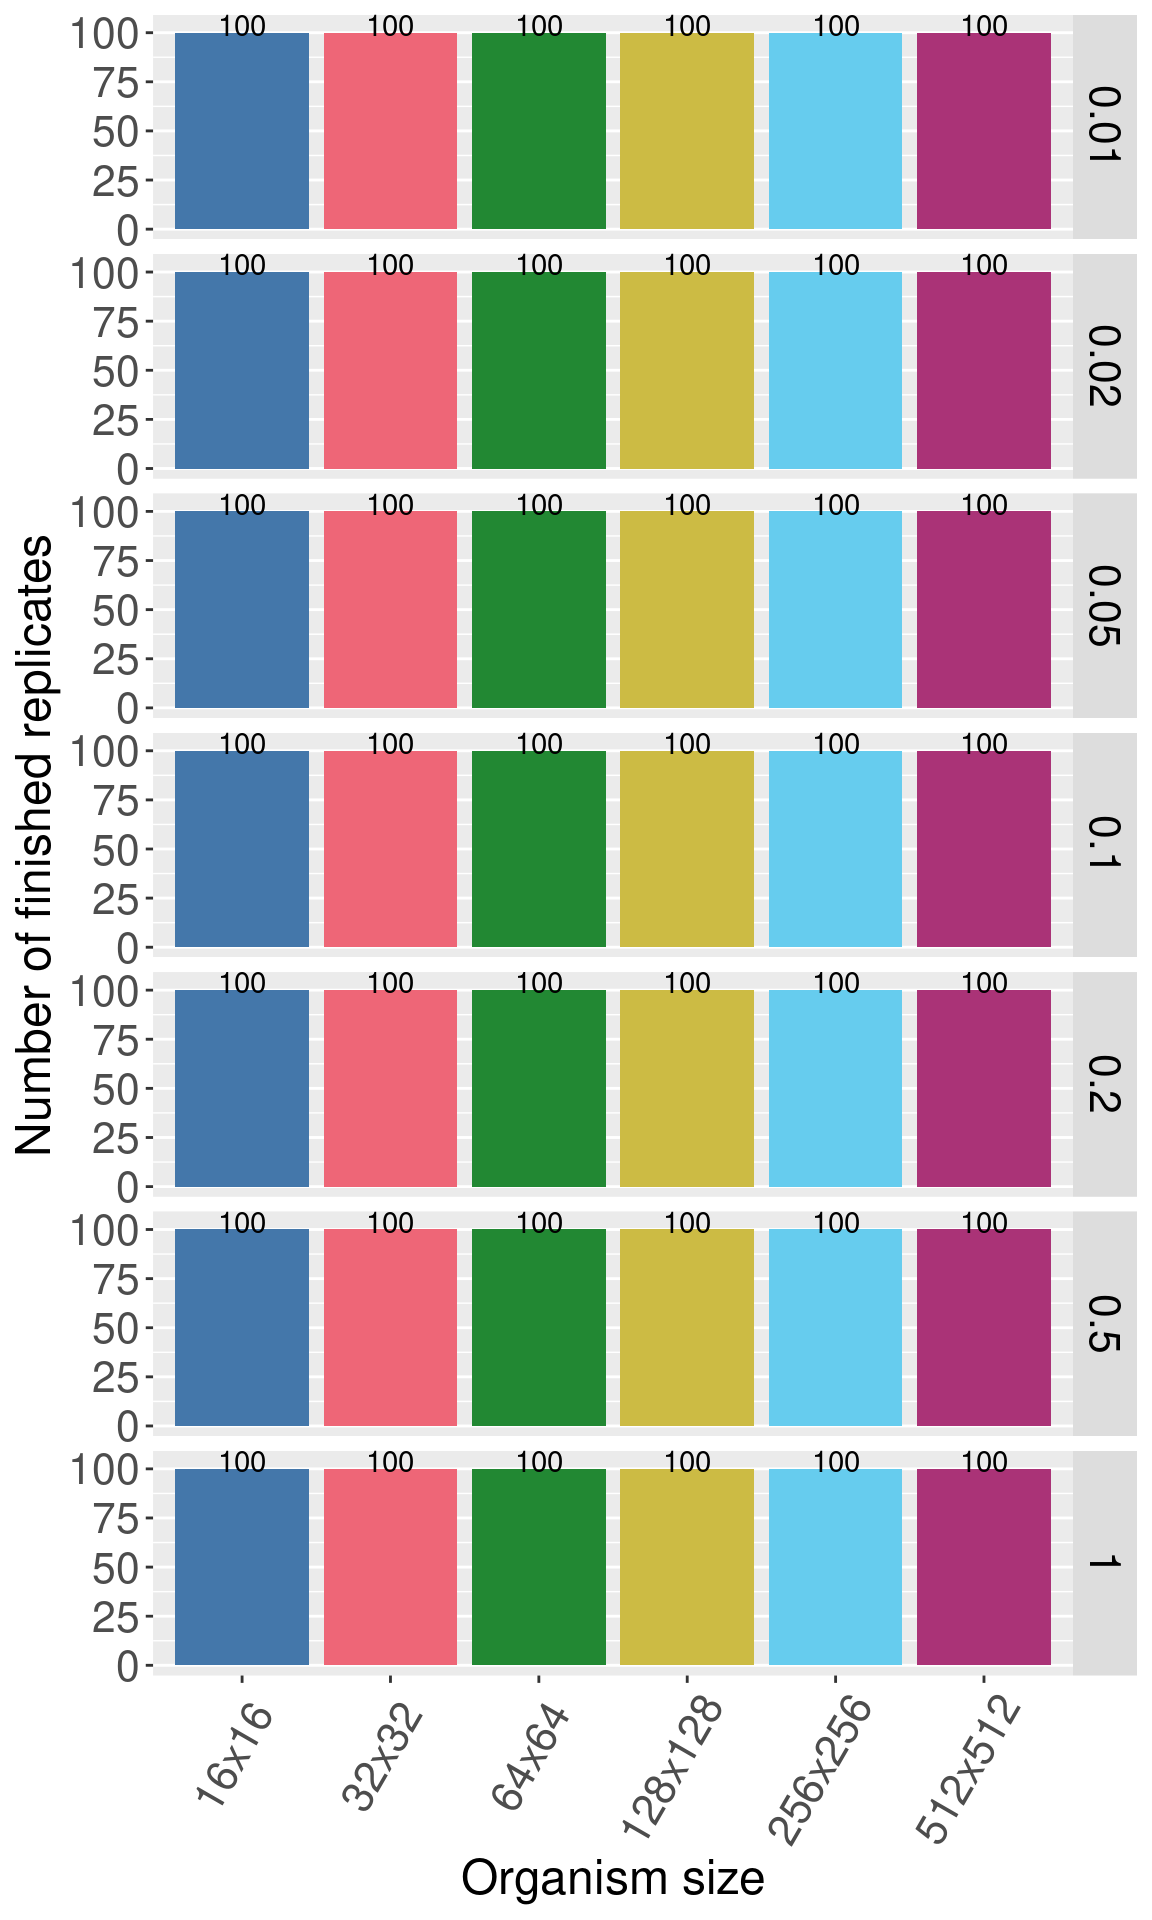
\includegraphics{primordium_supplemental_material_files/figure-latex/unnamed-chunk-5-1.pdf}

\hypertarget{aggregate-plots}{%
\section{Aggregate plots}\label{aggregate-plots}}

Here we plot all the data at once.

\hypertarget{boxplots}{%
\subsection{Boxplots}\label{boxplots}}

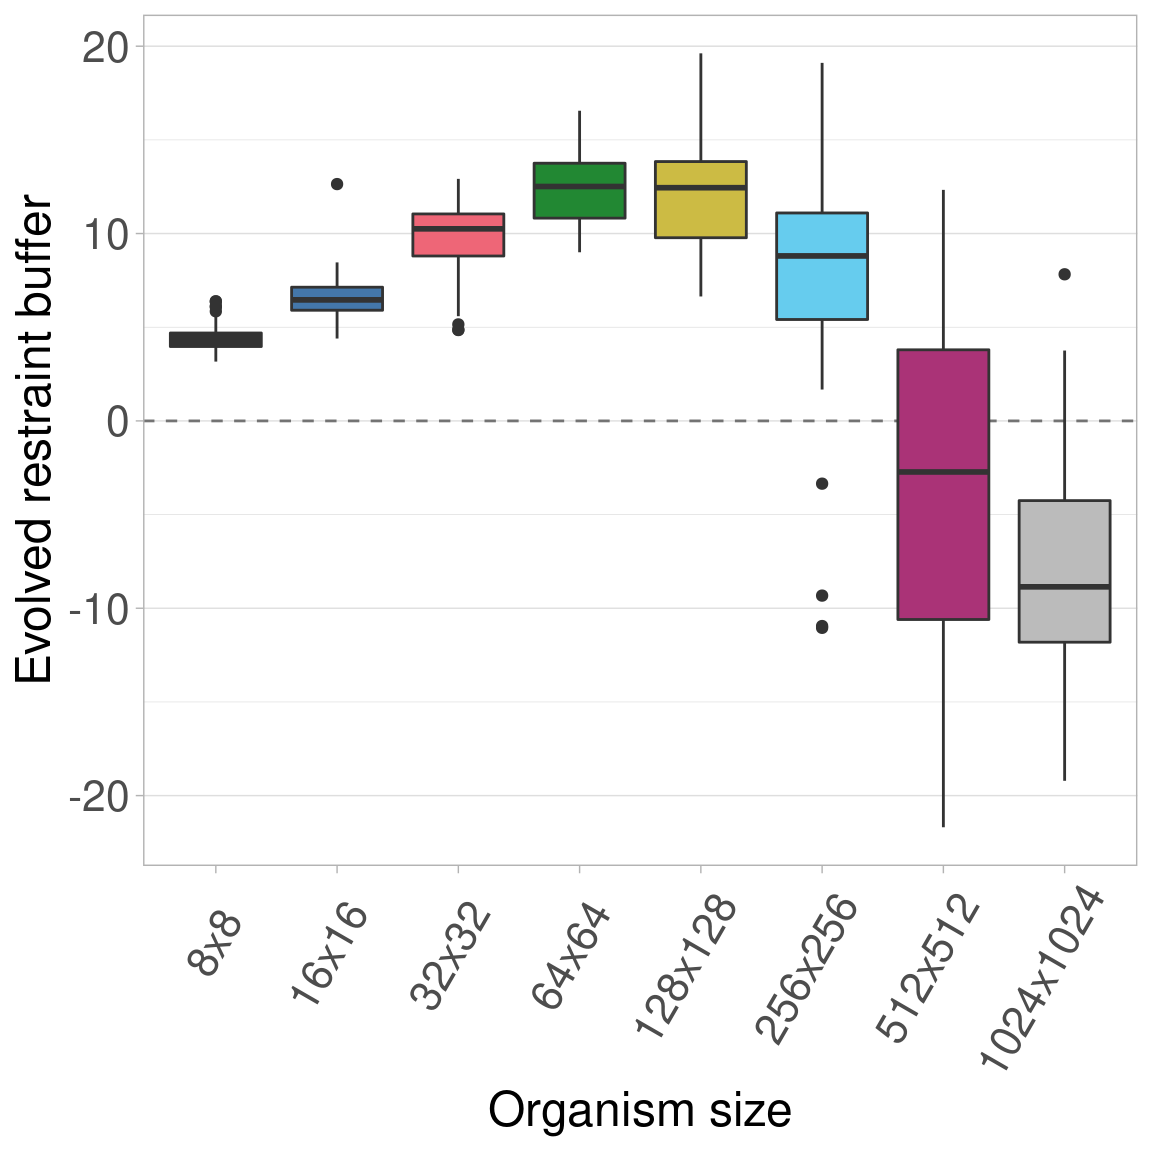
\includegraphics{primordium_supplemental_material_files/figure-latex/unnamed-chunk-6-1.pdf}

\hypertarget{raincloud-plots}{%
\subsection{Raincloud plots}\label{raincloud-plots}}

We can plot the same data via raincloud plots.

\begin{verbatim}
## Picking joint bandwidth of 1.16
\end{verbatim}

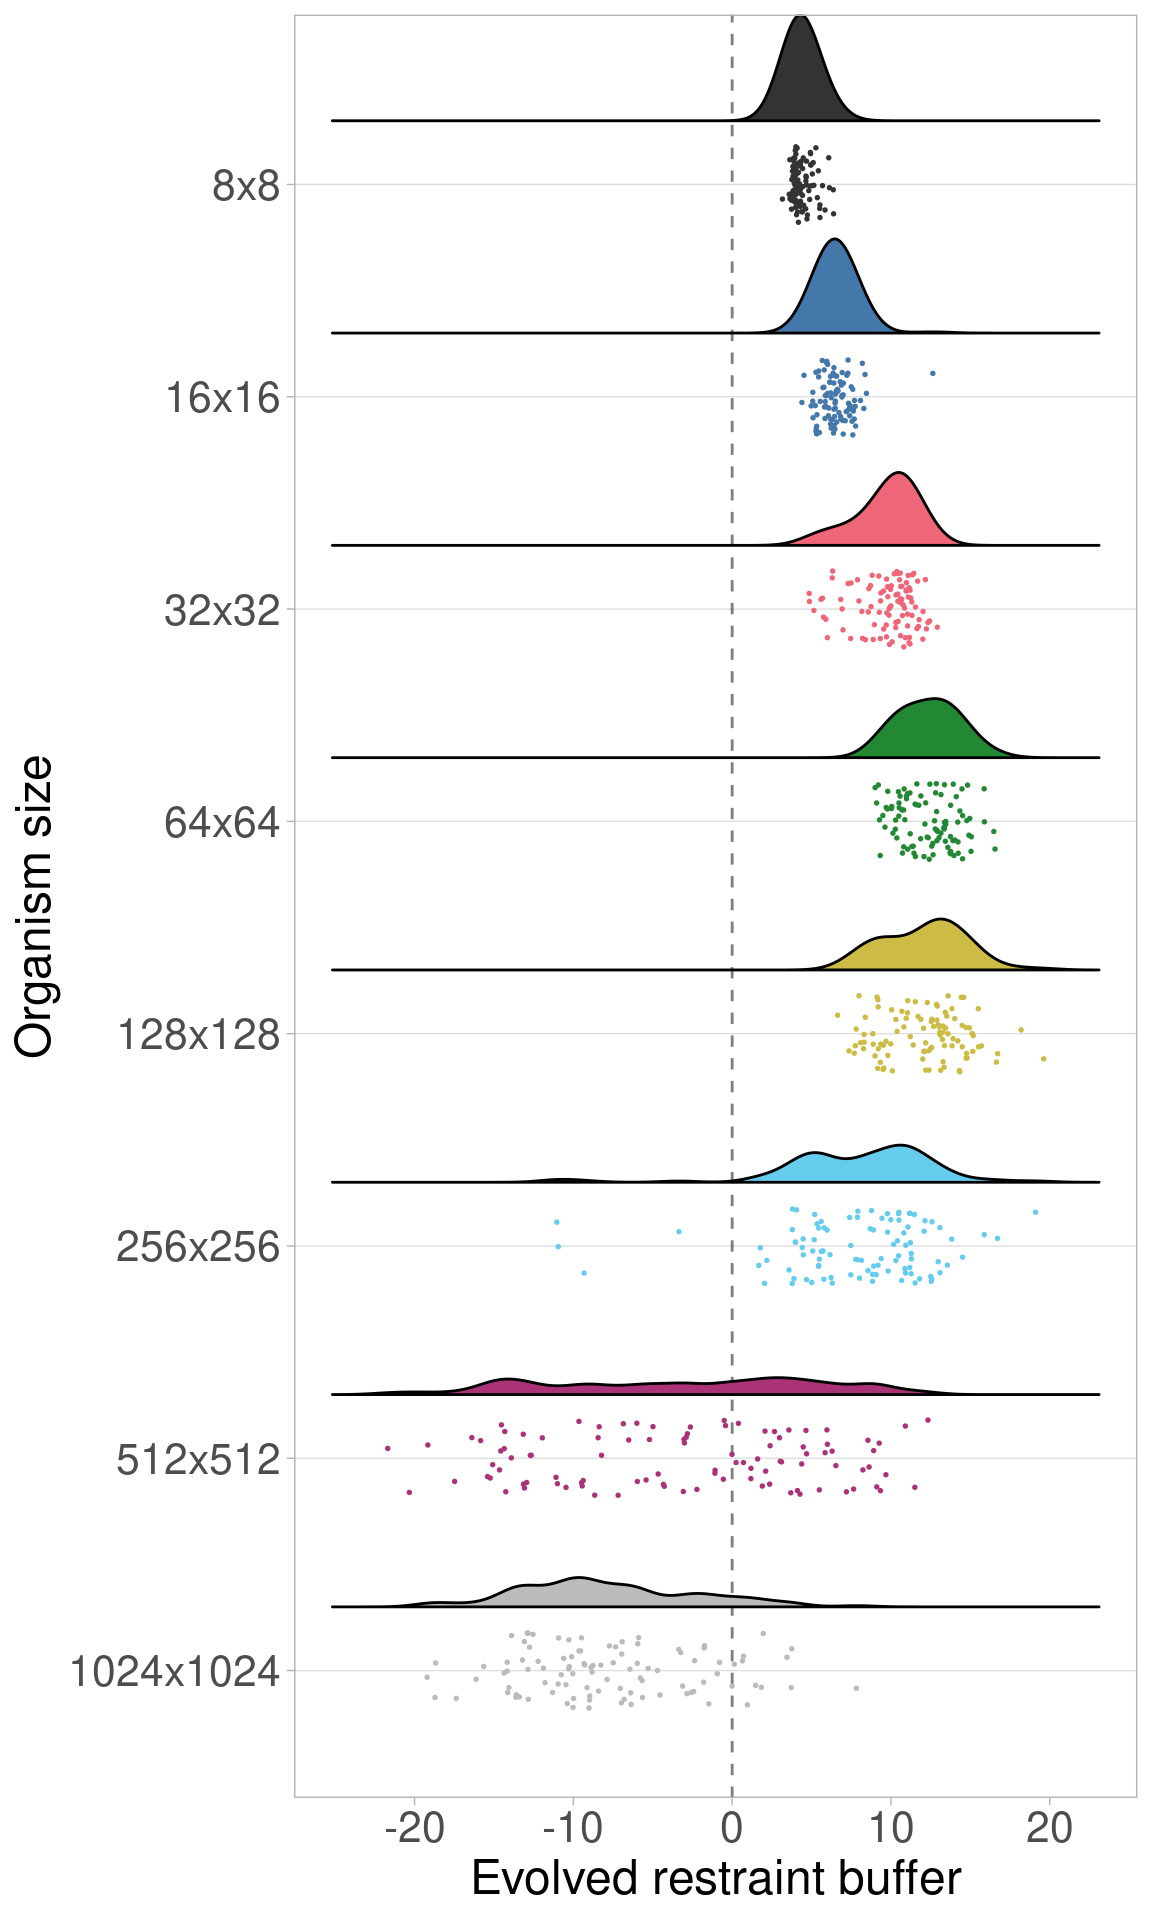
\includegraphics{primordium_supplemental_material_files/figure-latex/unnamed-chunk-7-1.pdf}

\hypertarget{statistics}{%
\section{Statistics}\label{statistics}}

First, we perform a Kruskal-Wallis test across all organism sizes to indicate if variance exists.
If variance exists, we then perform a pairwise Wilcoxon Rank-Sum test to show which pairs of organism sizes significantly differ.
Finally, we perform Bonferroni-Holm corrections for multiple comparisons.

\begin{Shaded}
\begin{Highlighting}[]
\NormalTok{  res =}\StringTok{ }\KeywordTok{kruskal.test}\NormalTok{(df2}\OperatorTok{$}\NormalTok{restraint_value }\OperatorTok{~}\StringTok{ }\NormalTok{df2}\OperatorTok{$}\NormalTok{MCSIZE, df2)}
\NormalTok{  df_kruskal =}\StringTok{ }\KeywordTok{data.frame}\NormalTok{(}\DataTypeTok{data =} \KeywordTok{matrix}\NormalTok{(}\DataTypeTok{nrow =} \DecValTok{0}\NormalTok{, }\DataTypeTok{ncol =} \DecValTok{3}\NormalTok{))}
  \KeywordTok{colnames}\NormalTok{(df_kruskal) =}\StringTok{ }\KeywordTok{c}\NormalTok{(}\StringTok{'p_value'}\NormalTok{, }\StringTok{'chi_squared'}\NormalTok{, }\StringTok{'df'}\NormalTok{)}
\NormalTok{  df_kruskal[}\KeywordTok{nrow}\NormalTok{(df_kruskal) }\OperatorTok{+}\StringTok{ }\DecValTok{1}\NormalTok{,] =}\StringTok{ }\KeywordTok{c}\NormalTok{(res}\OperatorTok{$}\NormalTok{p.value, }\KeywordTok{as.numeric}\NormalTok{(res}\OperatorTok{$}\NormalTok{statistic)[}\DecValTok{1}\NormalTok{], }\KeywordTok{as.numeric}\NormalTok{(res}\OperatorTok{$}\NormalTok{parameter)[}\DecValTok{1}\NormalTok{])}
\NormalTok{  df_kruskal}\OperatorTok{$}\NormalTok{less_}\FloatTok{0.01}\NormalTok{ =}\StringTok{ }\NormalTok{df_kruskal}\OperatorTok{$}\NormalTok{p_value }\OperatorTok{<}\StringTok{ }\FloatTok{0.01}
  \KeywordTok{print}\NormalTok{(df_kruskal)}
\end{Highlighting}
\end{Shaded}

\begin{verbatim}
##         p_value chi_squared df less_0.01
## 1 1.506351e-127    610.2553  7      TRUE
\end{verbatim}

We see that significant variation exists, so we perform pariwise Wilcoxon tests on each to see which pais of sizes are significantly different.

\begin{Shaded}
\begin{Highlighting}[]
\NormalTok{size_vec =}\StringTok{ }\KeywordTok{c}\NormalTok{(}\DecValTok{16}\NormalTok{, }\DecValTok{32}\NormalTok{, }\DecValTok{64}\NormalTok{, }\DecValTok{128}\NormalTok{, }\DecValTok{256}\NormalTok{, }\DecValTok{512}\NormalTok{)}
\NormalTok{df_test =}\StringTok{ }\NormalTok{df2}
\NormalTok{df_wilcox =}\StringTok{ }\KeywordTok{data.frame}\NormalTok{(}\DataTypeTok{data =} \KeywordTok{matrix}\NormalTok{(}\DataTypeTok{nrow =} \DecValTok{0}\NormalTok{, }\DataTypeTok{ncol =} \DecValTok{5}\NormalTok{))}
\KeywordTok{colnames}\NormalTok{(df_wilcox) =}\StringTok{ }\KeywordTok{c}\NormalTok{(}\StringTok{'size_a'}\NormalTok{, }\StringTok{'size_b'}\NormalTok{, }\StringTok{'p_value_corrected'}\NormalTok{, }\StringTok{'p_value_raw'}\NormalTok{, }\StringTok{'W'}\NormalTok{)}
\ControlFlowTok{for}\NormalTok{(size_idx_a }\ControlFlowTok{in} \DecValTok{1}\OperatorTok{:}\NormalTok{(}\KeywordTok{length}\NormalTok{(size_vec) }\OperatorTok{-}\StringTok{ }\DecValTok{1}\NormalTok{))\{}
\NormalTok{  size_a =}\StringTok{ }\NormalTok{size_vec[size_idx_a]}
  \ControlFlowTok{for}\NormalTok{(size_idx_b }\ControlFlowTok{in}\NormalTok{ (size_idx_a }\OperatorTok{+}\StringTok{ }\DecValTok{1}\NormalTok{)}\OperatorTok{:}\KeywordTok{length}\NormalTok{(size_vec))\{}
\NormalTok{    size_b =}\StringTok{ }\NormalTok{size_vec[size_idx_b]}
\NormalTok{    res =}\StringTok{ }\KeywordTok{wilcox.test}\NormalTok{(df_test[df_test}\OperatorTok{$}\NormalTok{MCSIZE }\OperatorTok{==}\StringTok{ }\NormalTok{size_a,]}\OperatorTok{$}\NormalTok{restraint_value, df_test[df_test}\OperatorTok{$}\NormalTok{MCSIZE }\OperatorTok{==}\StringTok{ }\NormalTok{size_b,]}\OperatorTok{$}\NormalTok{restraint_value, }\DataTypeTok{alternative =} \StringTok{'two.sided'}\NormalTok{) }
\NormalTok{    df_wilcox[}\KeywordTok{nrow}\NormalTok{(df_wilcox) }\OperatorTok{+}\StringTok{ }\DecValTok{1}\NormalTok{,] =}\StringTok{ }\KeywordTok{c}\NormalTok{(size_a, size_b, }\DecValTok{0}\NormalTok{, res}\OperatorTok{$}\NormalTok{p.value, }\KeywordTok{as.numeric}\NormalTok{(res}\OperatorTok{$}\NormalTok{statistic)[}\DecValTok{1}\NormalTok{])}
\NormalTok{  \}}
\NormalTok{\}}
\NormalTok{df_wilcox}\OperatorTok{$}\NormalTok{p_value_corrected =}\StringTok{ }\KeywordTok{p.adjust}\NormalTok{(df_wilcox}\OperatorTok{$}\NormalTok{p_value_raw, }\DataTypeTok{method =} \StringTok{'holm'}\NormalTok{)}
\NormalTok{df_wilcox}\OperatorTok{$}\NormalTok{less_}\FloatTok{0.01}\NormalTok{ =}\StringTok{ }\NormalTok{df_wilcox}\OperatorTok{$}\NormalTok{p_value_corrected }\OperatorTok{<}\StringTok{ }\FloatTok{0.01}
\KeywordTok{print}\NormalTok{(df_wilcox)}
\end{Highlighting}
\end{Shaded}

\begin{verbatim}
##    size_a size_b p_value_corrected  p_value_raw      W less_0.01
## 1      16     32      4.406735e-21 4.406735e-22 1045.5      TRUE
## 2      16     64      1.790650e-32 1.193767e-33   51.5      TRUE
## 3      16    128      2.585339e-31 1.988723e-32  147.0      TRUE
## 4      16    256      1.864978e-03 6.216595e-04 3599.0      TRUE
## 5      16    512      3.596138e-17 4.495172e-18 8547.0      TRUE
## 6      32     64      2.103060e-15 3.004372e-16 1654.5      TRUE
## 7      32    128      1.857809e-09 4.644523e-10 2449.5      TRUE
## 8      32    256      8.472946e-03 4.236473e-03 6171.0      TRUE
## 9      32    512      1.338207e-26 1.216552e-27 9459.5      TRUE
## 10     64    128      4.429461e-01 4.429461e-01 5314.5     FALSE
## 11     64    256      2.515682e-15 4.192803e-16 8329.0      TRUE
## 12     64    512      1.552625e-31 1.109018e-32 9873.0      TRUE
## 13    128    256      4.763656e-12 9.527311e-13 7921.5      TRUE
## 14    128    512      3.610598e-30 3.008832e-31 9759.0      TRUE
## 15    256    512      7.155324e-19 7.950361e-20 8730.5      TRUE
\end{verbatim}

\hypertarget{somatic-mutation-rate-sweep}{%
\chapter{Somatic Mutation Rate Sweep}\label{somatic-mutation-rate-sweep}}

This experiment was one of the prelimary experiments we conducted to find the default parameters for Primordium.
Here, we vary the somatic mutation rate, the probability that a cell replication will result in the offspring cell having a different restraint value from its parent.

We settled on a somatic mutation rate of 0.5 (\emph{i.e.}, each cell replication has a 50\% chance of mutation).

The configuration script and data for the experiment can be found under \texttt{2021\_02\_27\_\_soma\_mut\_fin/} in the experiments directory of the git repository.

\hypertarget{data-cleaning-1}{%
\section{Data cleaning}\label{data-cleaning-1}}

Load necessary libraries

\begin{Shaded}
\begin{Highlighting}[]
\KeywordTok{library}\NormalTok{(dplyr)}
\KeywordTok{library}\NormalTok{(ggplot2)}
\KeywordTok{library}\NormalTok{(ggridges)}
\KeywordTok{library}\NormalTok{(scales)}
\KeywordTok{library}\NormalTok{(khroma)}
\end{Highlighting}
\end{Shaded}

Load the data and trim all the unecessay bits (\emph{e.g.}, we initially ran sizes 8x8, 1024x1024 but cut them from the paper to make plots easier to read).

\begin{Shaded}
\begin{Highlighting}[]
\CommentTok{# Load the data}
\NormalTok{df =}\StringTok{ }\KeywordTok{read.csv}\NormalTok{(}\StringTok{'../experiments/2021_02_27__soma_mut_fin/evolution/data/scraped_evolution_data.csv'}\NormalTok{)}
\CommentTok{# Trim off NAs (artifiacts of how we scraped the data) and trim to only have gen 10,000}
\NormalTok{df2 =}\StringTok{ }\NormalTok{df[}\OperatorTok{!}\KeywordTok{is.na}\NormalTok{(df}\OperatorTok{$}\NormalTok{MCSIZE) }\OperatorTok{&}\StringTok{ }\NormalTok{df}\OperatorTok{$}\NormalTok{generation }\OperatorTok{==}\StringTok{ }\DecValTok{10000}\NormalTok{,]}
\CommentTok{# Ignore data for size 8x8 and 1024x1024}
\NormalTok{df2 =}\StringTok{ }\NormalTok{df2[df2}\OperatorTok{$}\NormalTok{MCSIZE }\OperatorTok{!=}\StringTok{ }\DecValTok{8} \OperatorTok{&}\StringTok{ }\NormalTok{df2}\OperatorTok{$}\NormalTok{MCSIZE }\OperatorTok{!=}\StringTok{ }\DecValTok{1024}\NormalTok{,]}
\end{Highlighting}
\end{Shaded}

We group and summarize the data to make to ensure all replicates are present.

\begin{Shaded}
\begin{Highlighting}[]
\CommentTok{# Group the data by size and summarize}
\NormalTok{data_grouped =}\StringTok{ }\NormalTok{dplyr}\OperatorTok{::}\KeywordTok{group_by}\NormalTok{(df2, MCSIZE, CELLMUT)}
\NormalTok{data_summary =}\StringTok{ }\NormalTok{dplyr}\OperatorTok{::}\KeywordTok{summarize}\NormalTok{(data_grouped, }\DataTypeTok{mean_ones =} \KeywordTok{mean}\NormalTok{(ave_ones), }\DataTypeTok{n =}\NormalTok{ dplyr}\OperatorTok{::}\KeywordTok{n}\NormalTok{())}
\end{Highlighting}
\end{Shaded}

We clean the data and create a few helper variables to make plotting easier.

\begin{Shaded}
\begin{Highlighting}[]
\CommentTok{# Calculate restraint value (x - 60 because genome length is 100 here)}
\NormalTok{df2}\OperatorTok{$}\NormalTok{restraint_value =}\StringTok{ }\NormalTok{df2}\OperatorTok{$}\NormalTok{ave_ones }\OperatorTok{-}\StringTok{ }\DecValTok{60}
\CommentTok{# Make a nice, clean factor for size}
\NormalTok{df2}\OperatorTok{$}\NormalTok{size_str =}\StringTok{ }\KeywordTok{paste0}\NormalTok{(df2}\OperatorTok{$}\NormalTok{MCSIZE, }\StringTok{'x'}\NormalTok{, df2}\OperatorTok{$}\NormalTok{MCSIZE)}
\NormalTok{df2}\OperatorTok{$}\NormalTok{size_factor =}\StringTok{ }\KeywordTok{factor}\NormalTok{(df2}\OperatorTok{$}\NormalTok{size_str, }\DataTypeTok{levels =} \KeywordTok{c}\NormalTok{(}\StringTok{'16x16'}\NormalTok{, }\StringTok{'32x32'}\NormalTok{, }\StringTok{'64x64'}\NormalTok{, }\StringTok{'128x128'}\NormalTok{, }\StringTok{'256x256'}\NormalTok{, }\StringTok{'512x512'}\NormalTok{, }\StringTok{'1024x1024'}\NormalTok{))}
\NormalTok{df2}\OperatorTok{$}\NormalTok{size_factor_reversed =}\StringTok{ }\KeywordTok{factor}\NormalTok{(df2}\OperatorTok{$}\NormalTok{size_str, }\DataTypeTok{levels =} \KeywordTok{rev}\NormalTok{(}\KeywordTok{c}\NormalTok{(}\StringTok{'16x16'}\NormalTok{, }\StringTok{'32x32'}\NormalTok{, }\StringTok{'64x64'}\NormalTok{, }\StringTok{'128x128'}\NormalTok{, }\StringTok{'256x256'}\NormalTok{, }\StringTok{'512x512'}\NormalTok{, }\StringTok{'1024x1024'}\NormalTok{)))}
\NormalTok{df2}\OperatorTok{$}\NormalTok{soma_mut_str =}\StringTok{ }\KeywordTok{paste}\NormalTok{(}\StringTok{'soma CELLMUT'}\NormalTok{, df2}\OperatorTok{$}\NormalTok{CELLMUT)}
\NormalTok{df2}\OperatorTok{$}\NormalTok{mut_factor =}\StringTok{ }\KeywordTok{factor}\NormalTok{(df2}\OperatorTok{$}\NormalTok{CELLMUT, }\DataTypeTok{levels =} \KeywordTok{c}\NormalTok{(}\FloatTok{0.01}\NormalTok{, }\FloatTok{0.02}\NormalTok{, }\FloatTok{0.05}\NormalTok{, }\FloatTok{0.10}\NormalTok{, }\FloatTok{0.20}\NormalTok{, }\FloatTok{0.50}\NormalTok{, }\FloatTok{1.00}\NormalTok{))}
\NormalTok{data_summary}\OperatorTok{$}\NormalTok{size_str =}\StringTok{ }\KeywordTok{paste0}\NormalTok{(data_summary}\OperatorTok{$}\NormalTok{MCSIZE, }\StringTok{'x'}\NormalTok{, data_summary}\OperatorTok{$}\NormalTok{MCSIZE)}
\NormalTok{data_summary}\OperatorTok{$}\NormalTok{size_factor =}\StringTok{ }\KeywordTok{factor}\NormalTok{(data_summary}\OperatorTok{$}\NormalTok{size_str, }\DataTypeTok{levels =} \KeywordTok{c}\NormalTok{(}\StringTok{'16x16'}\NormalTok{, }\StringTok{'32x32'}\NormalTok{, }\StringTok{'64x64'}\NormalTok{, }\StringTok{'128x128'}\NormalTok{, }\StringTok{'256x256'}\NormalTok{, }\StringTok{'512x512'}\NormalTok{, }\StringTok{'1024x1024'}\NormalTok{))}
\NormalTok{data_summary}\OperatorTok{$}\NormalTok{soma_mut_str =}\StringTok{ }\KeywordTok{paste}\NormalTok{(}\StringTok{'soma CELLMUT'}\NormalTok{, data_summary}\OperatorTok{$}\NormalTok{CELLMUT)}
\NormalTok{data_summary}\OperatorTok{$}\NormalTok{mut_factor =}\StringTok{ }\KeywordTok{factor}\NormalTok{(data_summary}\OperatorTok{$}\NormalTok{CELLMUT, }\DataTypeTok{levels =} \KeywordTok{c}\NormalTok{(}\FloatTok{0.01}\NormalTok{, }\FloatTok{0.02}\NormalTok{, }\FloatTok{0.05}\NormalTok{, }\FloatTok{0.10}\NormalTok{, }\FloatTok{0.20}\NormalTok{, }\FloatTok{0.50}\NormalTok{, }\FloatTok{1.00}\NormalTok{))}
\CommentTok{# Create a map of colors we'll use to plot the different organism sizes}
\NormalTok{color_vec =}\StringTok{ }\KeywordTok{as.character}\NormalTok{(khroma}\OperatorTok{::}\KeywordTok{color}\NormalTok{(}\StringTok{'bright'}\NormalTok{)(}\DecValTok{7}\NormalTok{))}
\NormalTok{color_map =}\StringTok{ }\KeywordTok{c}\NormalTok{(}
  \StringTok{'16x16'}\NormalTok{ =}\StringTok{     }\NormalTok{color_vec[}\DecValTok{1}\NormalTok{],}
  \StringTok{'32x32'}\NormalTok{ =}\StringTok{     }\NormalTok{color_vec[}\DecValTok{2}\NormalTok{],}
  \StringTok{'64x64'}\NormalTok{ =}\StringTok{     }\NormalTok{color_vec[}\DecValTok{3}\NormalTok{],}
  \StringTok{'128x128'}\NormalTok{ =}\StringTok{   }\NormalTok{color_vec[}\DecValTok{4}\NormalTok{],}
  \StringTok{'256x256'}\NormalTok{ =}\StringTok{   }\NormalTok{color_vec[}\DecValTok{5}\NormalTok{],}
  \StringTok{'512x512'}\NormalTok{ =}\StringTok{   }\NormalTok{color_vec[}\DecValTok{6}\NormalTok{],}
  \StringTok{'1024x1024'}\NormalTok{ =}\StringTok{ }\NormalTok{color_vec[}\DecValTok{7}\NormalTok{]}
\NormalTok{)}
\CommentTok{# Set the sizes for text in plots}
\NormalTok{text_major_size =}\StringTok{ }\DecValTok{18}
\NormalTok{text_minor_size =}\StringTok{ }\DecValTok{16} 
\end{Highlighting}
\end{Shaded}

\hypertarget{data-integrity-check-1}{%
\section{Data integrity check}\label{data-integrity-check-1}}

Now we plot the number of finished replicates for each treatment to make sure all data are present.
Each row shows a different somatic mutation rate.
Each bar/color shows a different organism size.
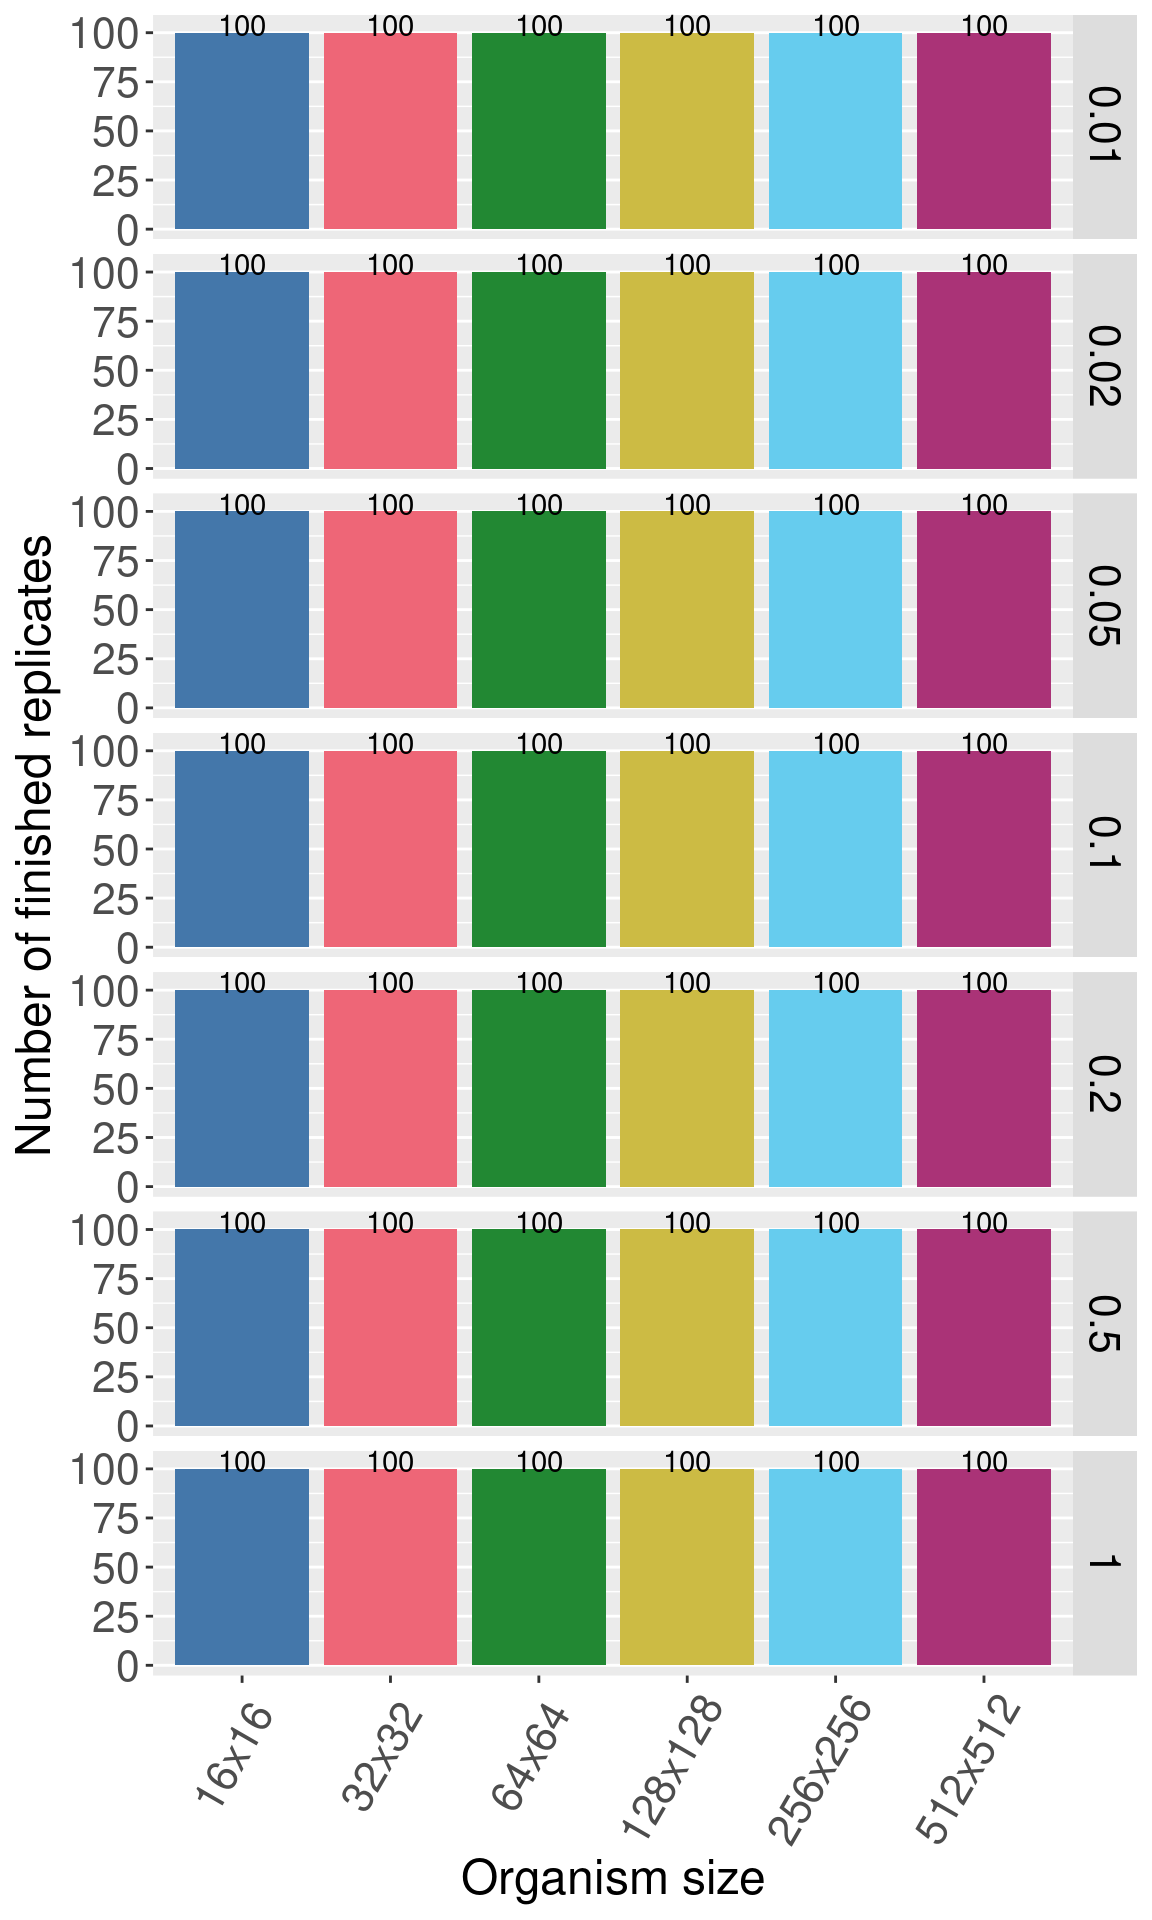
\includegraphics{primordium_supplemental_material_files/figure-latex/unnamed-chunk-14-1.pdf}

\hypertarget{aggregate-plots-1}{%
\section{Aggregate plots}\label{aggregate-plots-1}}

\hypertarget{facet-by-somatic-mutation-rate}{%
\subsection{Facet by somatic mutation rate}\label{facet-by-somatic-mutation-rate}}

Here we plot all the data at once.
Each row showing a different somatic mutation rate and each boxplot shows a given organism size.
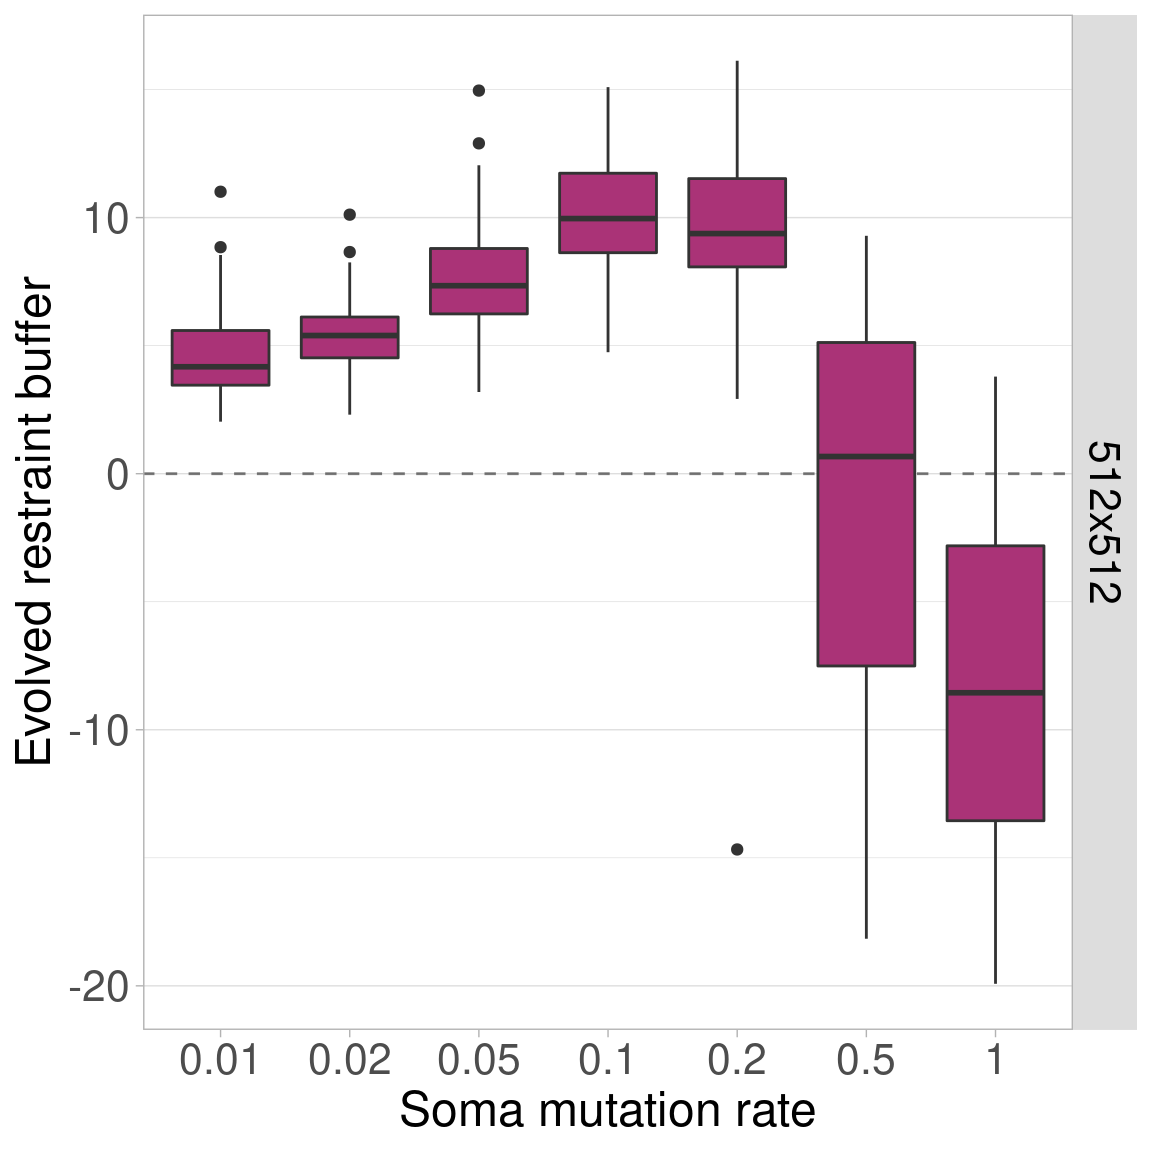
\includegraphics{primordium_supplemental_material_files/figure-latex/unnamed-chunk-15-1.pdf}

Here we plot the same data, only we allow the y-axis to vary between rows.
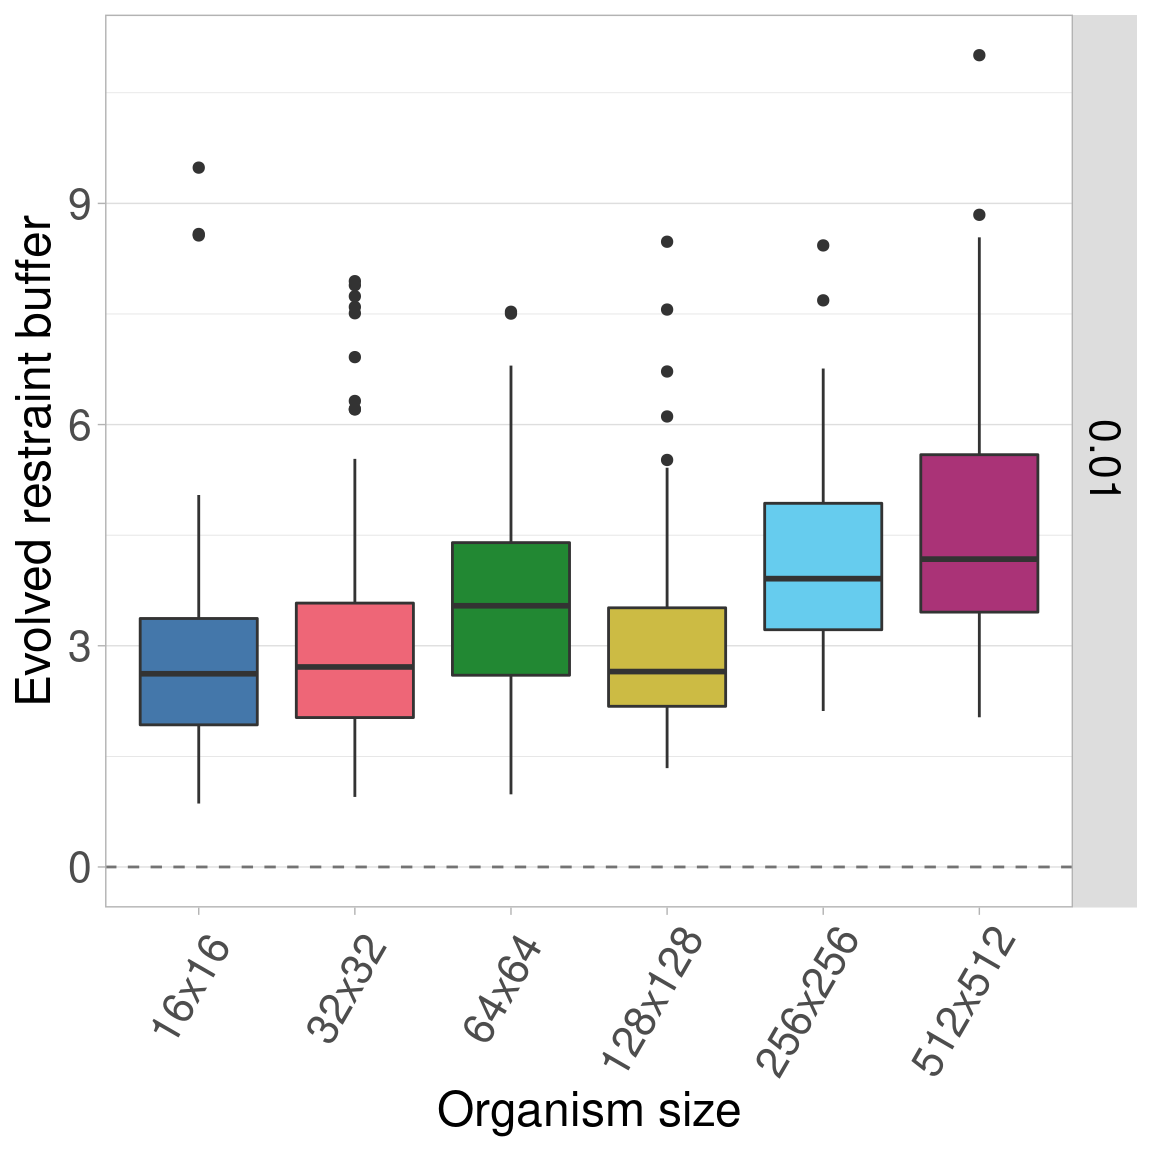
\includegraphics{primordium_supplemental_material_files/figure-latex/unnamed-chunk-16-1.pdf}

\hypertarget{facet-by-organism-size}{%
\subsection{Facet by organism size}\label{facet-by-organism-size}}

Next, we plot the same data, but this time each row corresponds to a certain organism size while somatic mutation rate changes along the x-axis.
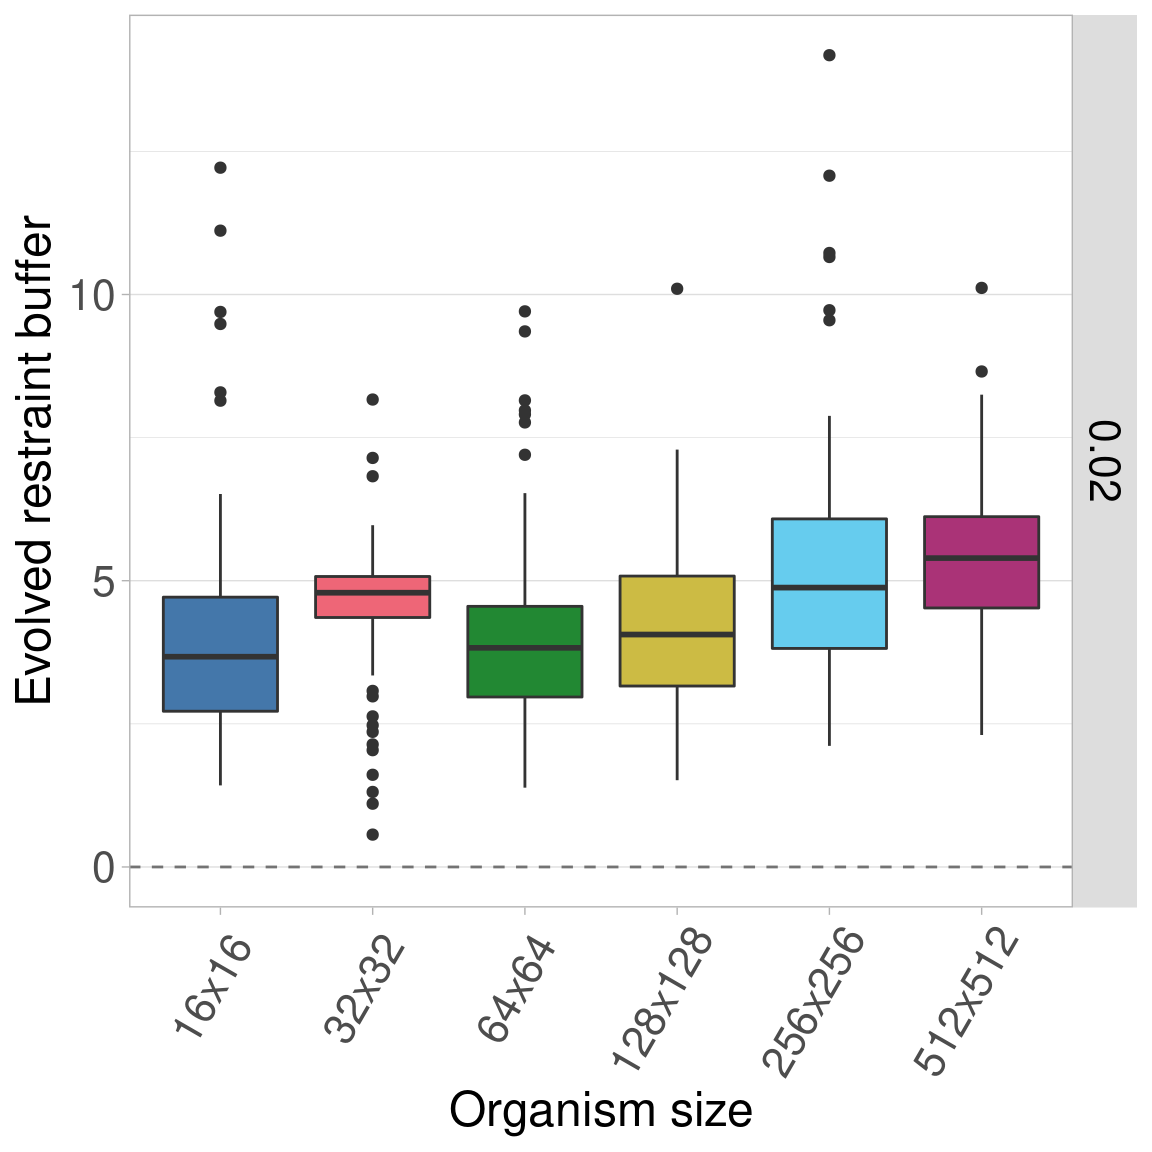
\includegraphics{primordium_supplemental_material_files/figure-latex/unnamed-chunk-17-1.pdf}

Again, we replot the same data but allow the y-axis to vary between rows.
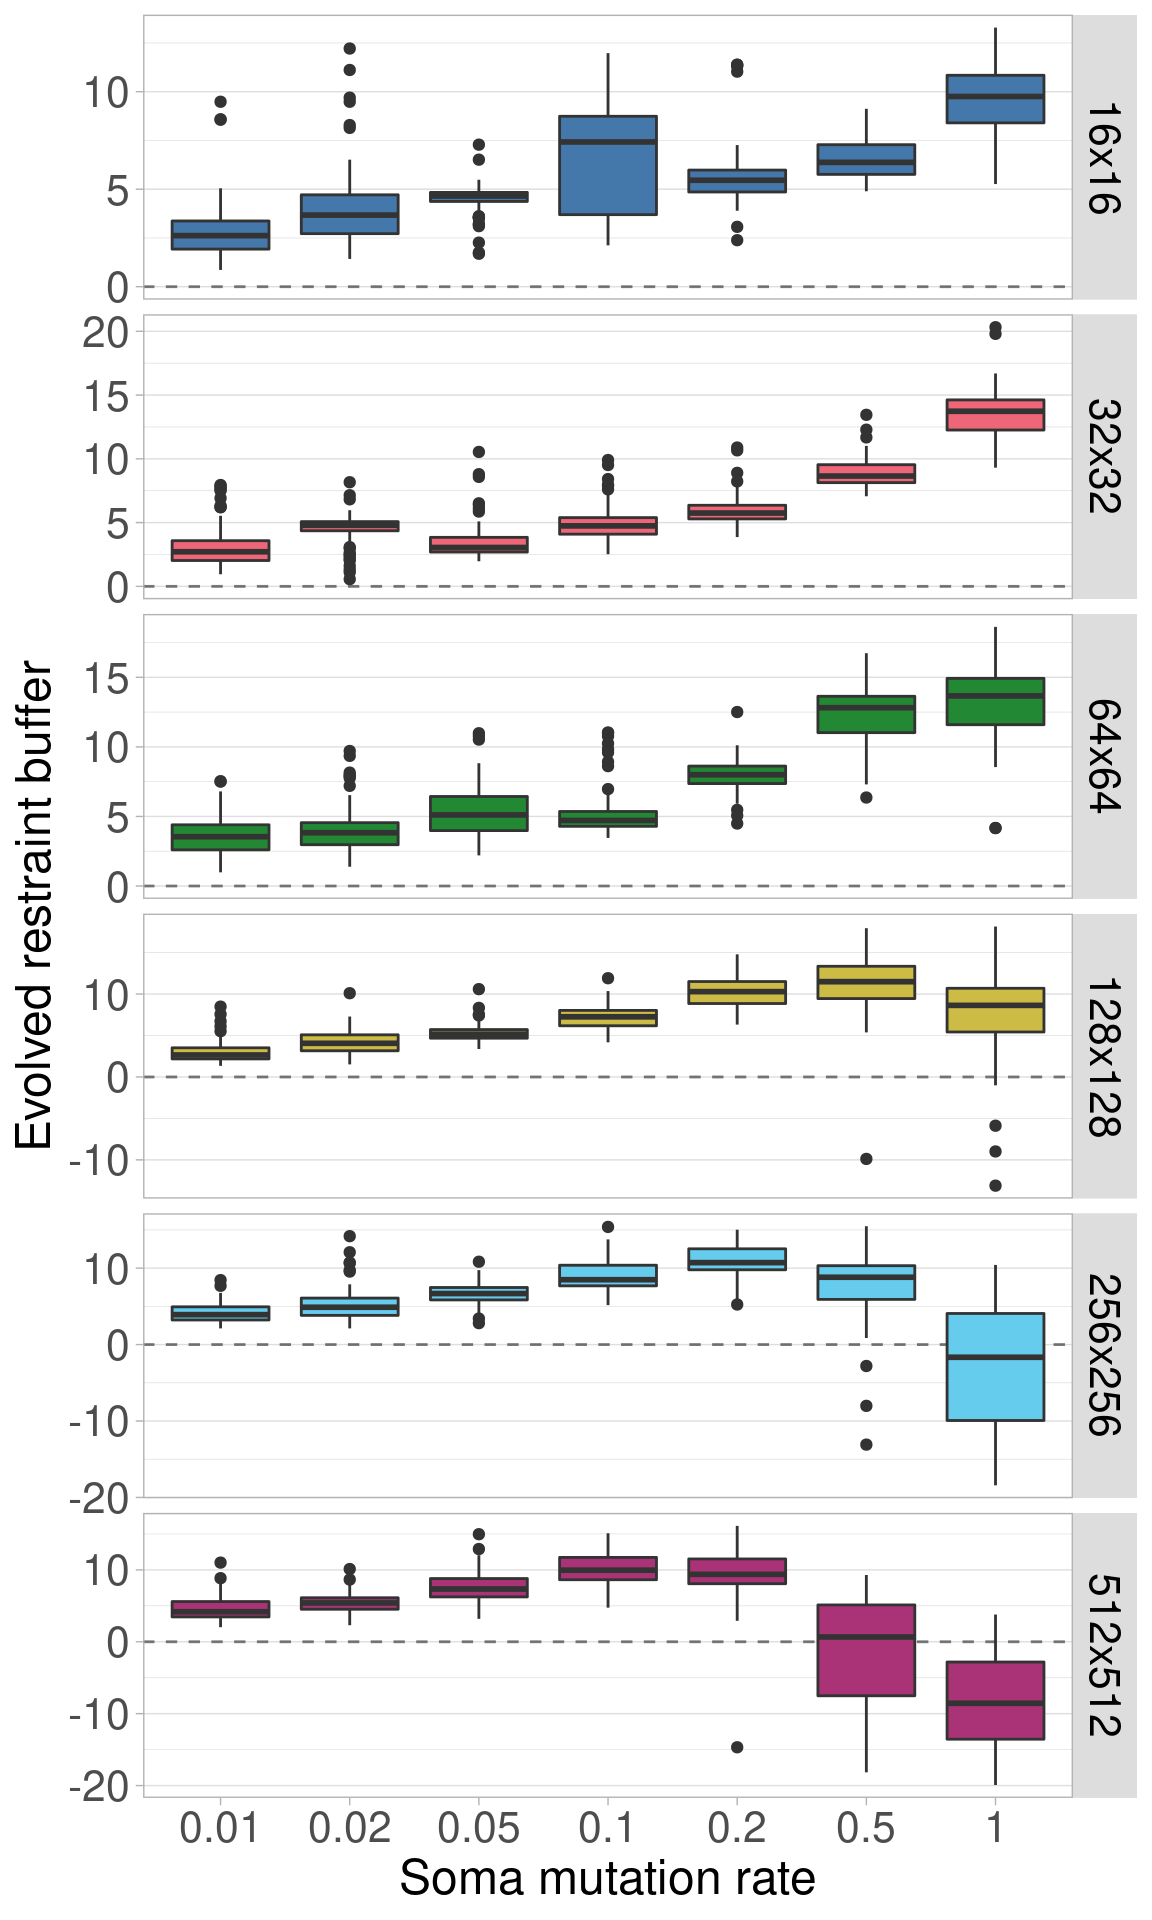
\includegraphics{primordium_supplemental_material_files/figure-latex/unnamed-chunk-18-1.pdf}

\hypertarget{single-organism-size-plots}{%
\section{Single organism size plots}\label{single-organism-size-plots}}

Here we plot each organism size independently, with the somatic mutation rate on the x-axis.

\hypertarget{organism-size-16x16}{%
\subsection{Organism size 16x16}\label{organism-size-16x16}}

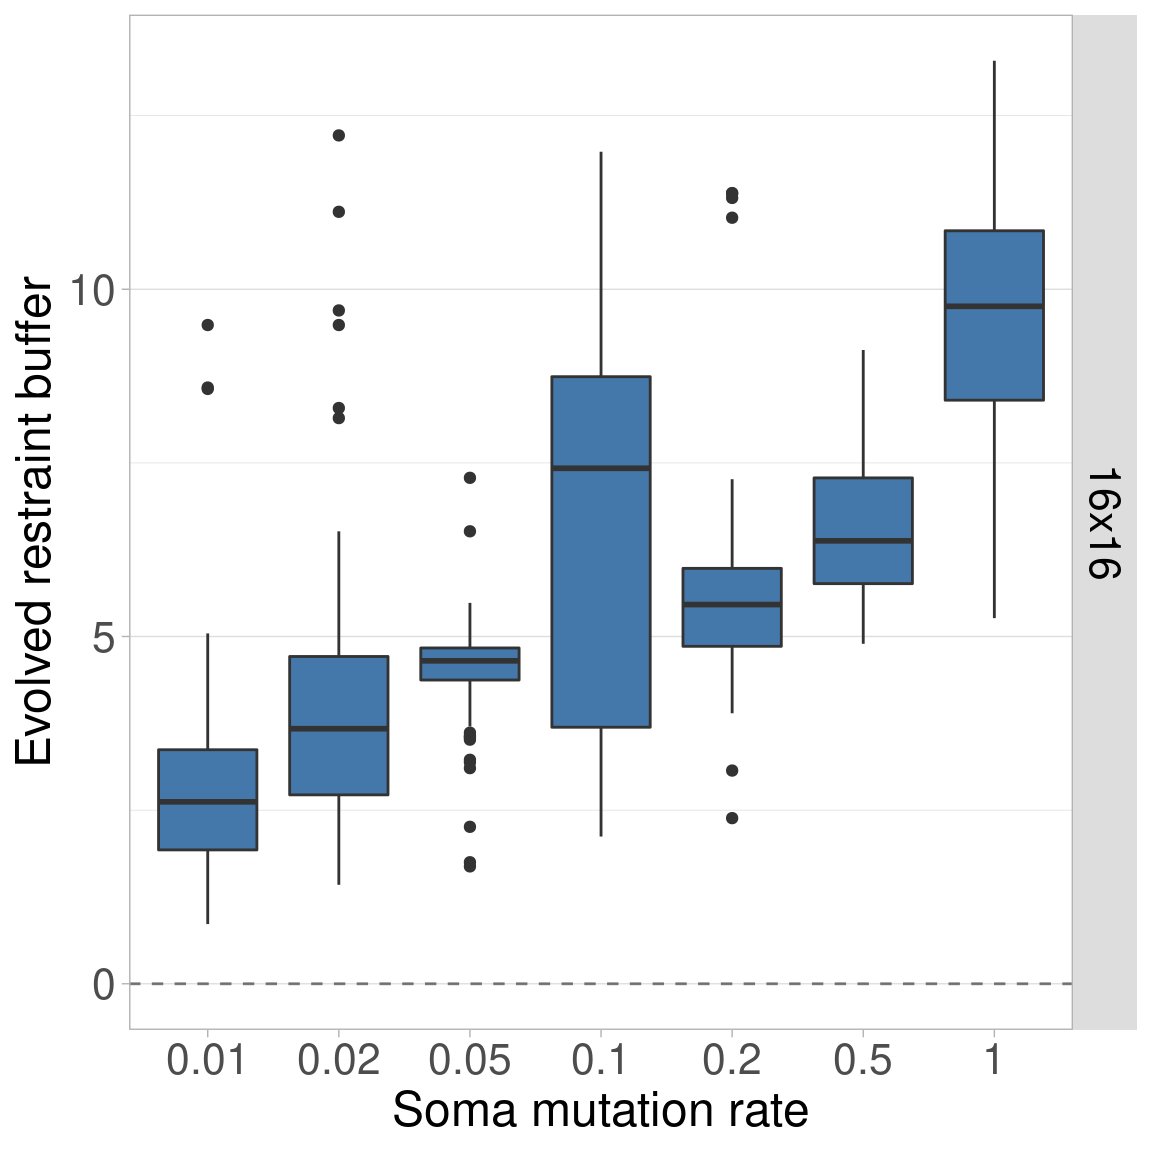
\includegraphics{primordium_supplemental_material_files/figure-latex/unnamed-chunk-19-1.pdf}

\hypertarget{organism-size-32x32}{%
\subsection{Organism size 32x32}\label{organism-size-32x32}}

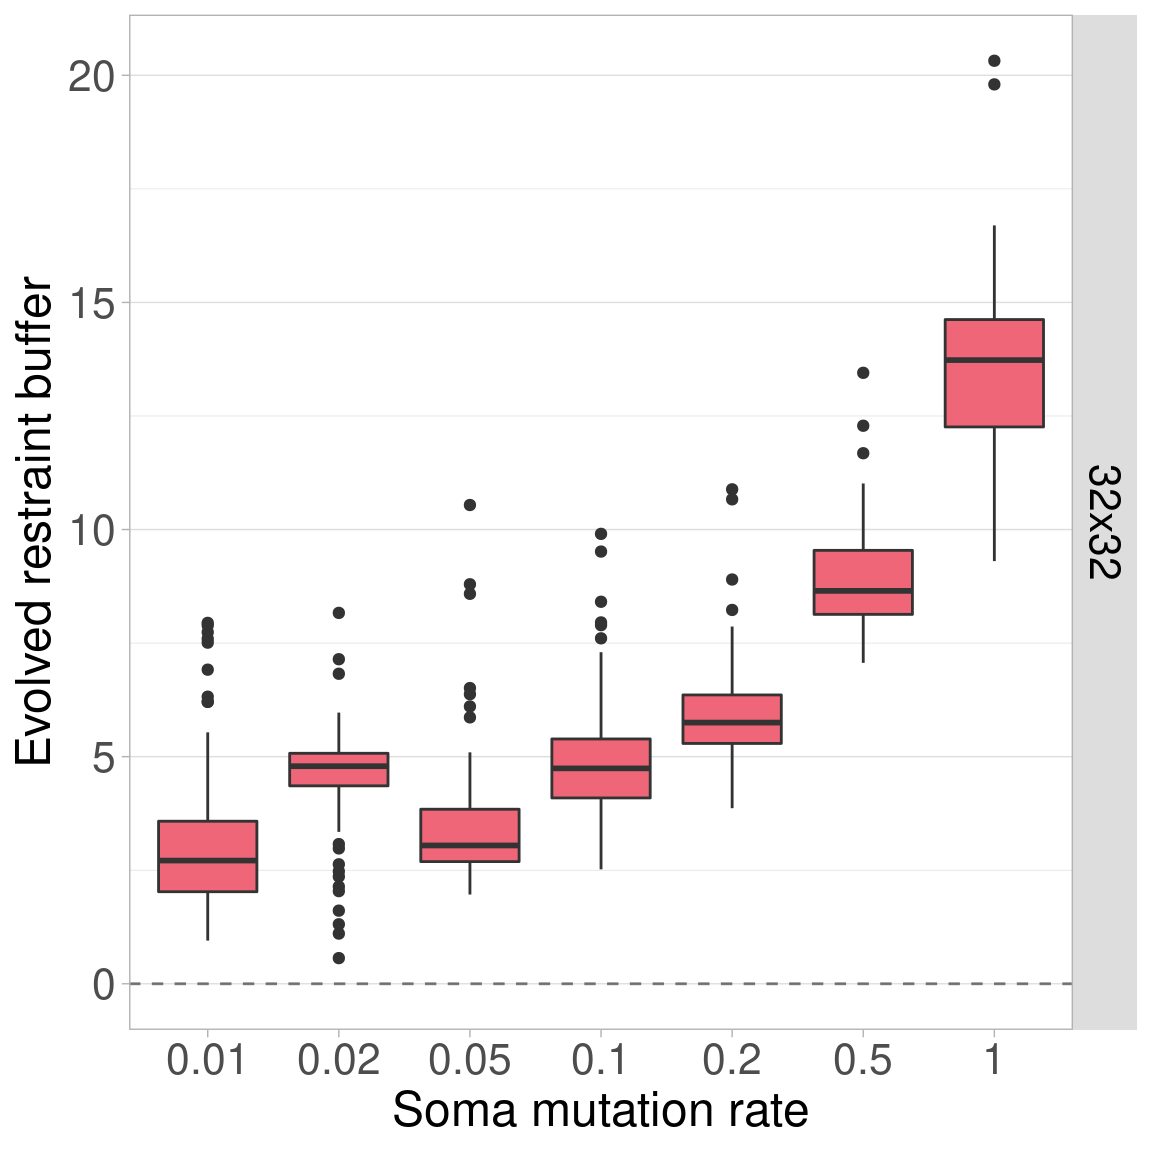
\includegraphics{primordium_supplemental_material_files/figure-latex/unnamed-chunk-20-1.pdf}

\hypertarget{organism-size-64x64}{%
\subsection{Organism size 64x64}\label{organism-size-64x64}}

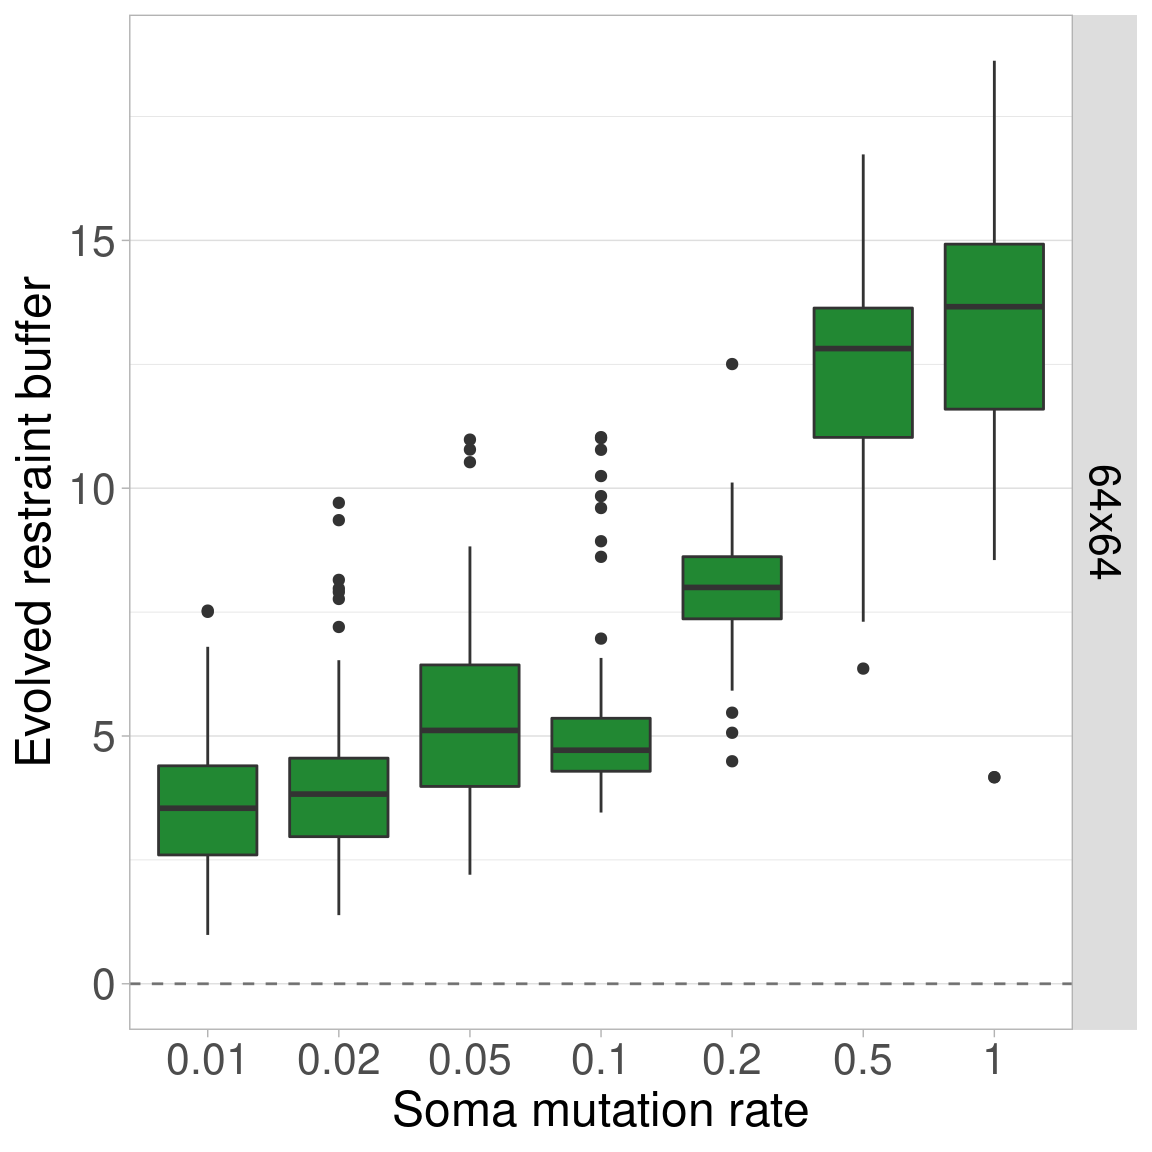
\includegraphics{primordium_supplemental_material_files/figure-latex/unnamed-chunk-21-1.pdf}

\hypertarget{organism-size-128x128}{%
\subsection{Organism size 128x128}\label{organism-size-128x128}}

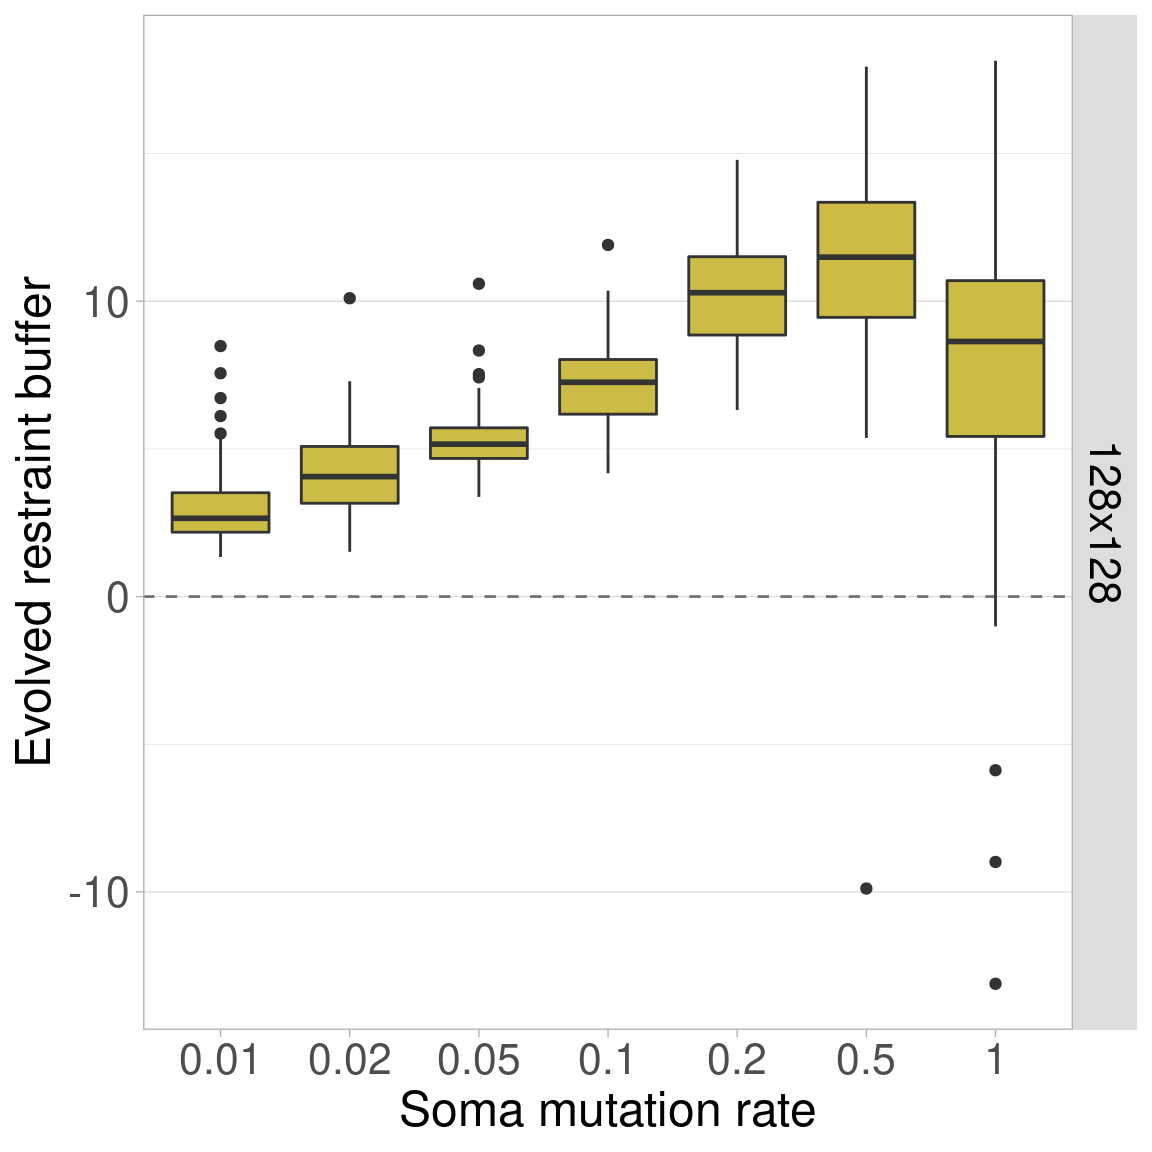
\includegraphics{primordium_supplemental_material_files/figure-latex/unnamed-chunk-22-1.pdf}

\hypertarget{organism-size-256x256}{%
\subsection{Organism size 256x256}\label{organism-size-256x256}}

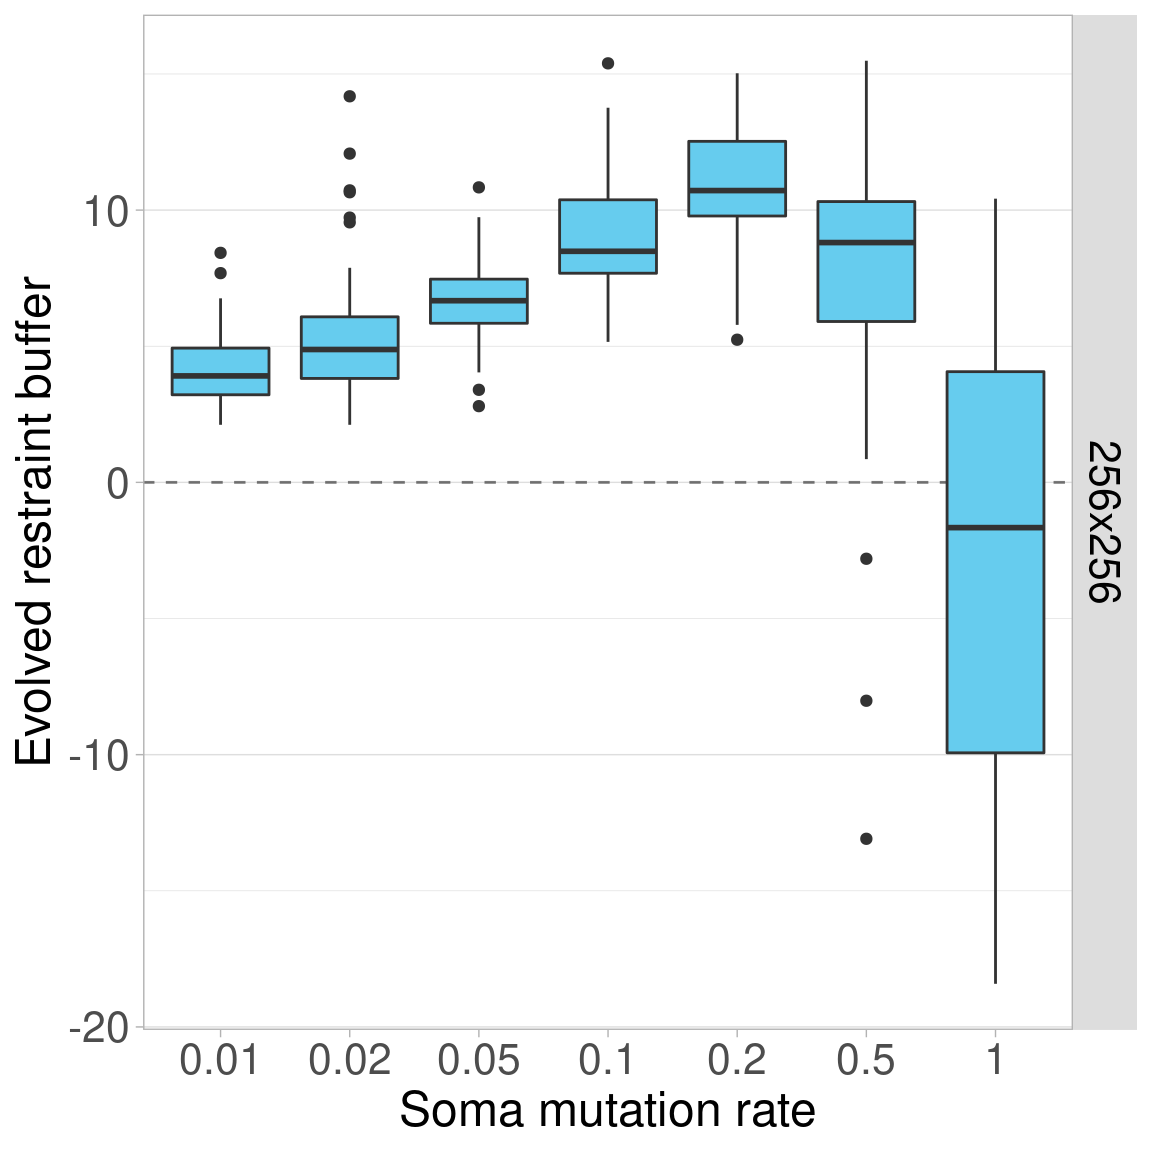
\includegraphics{primordium_supplemental_material_files/figure-latex/unnamed-chunk-23-1.pdf}

\hypertarget{organism-size-512x512}{%
\subsection{Organism size 512x512}\label{organism-size-512x512}}

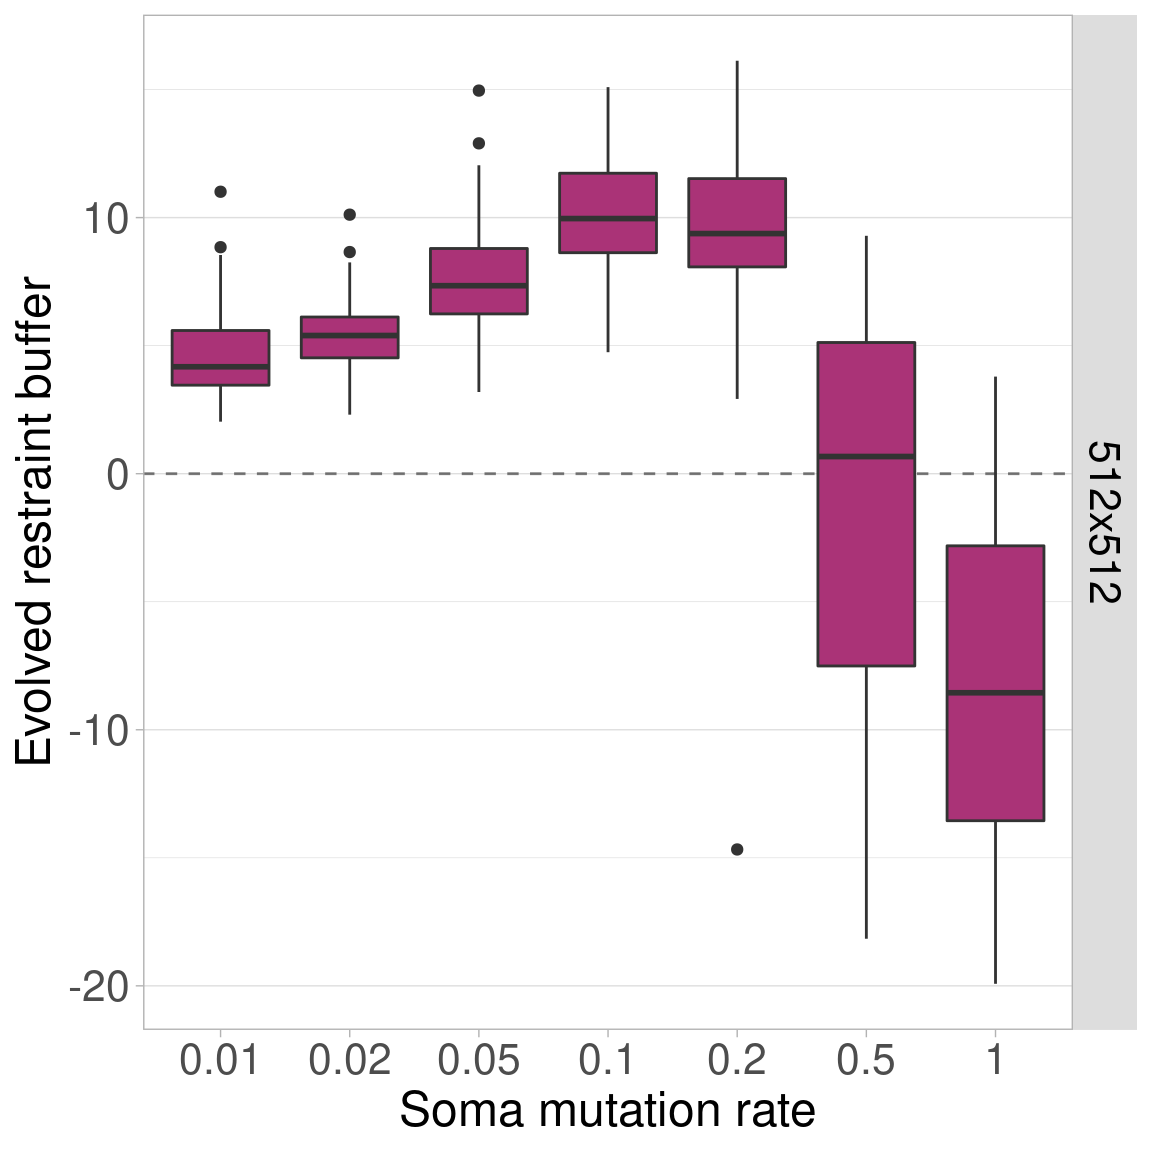
\includegraphics{primordium_supplemental_material_files/figure-latex/unnamed-chunk-24-1.pdf}

\hypertarget{single-somatic-mutation-rate-plots}{%
\section{Single somatic mutation rate plots}\label{single-somatic-mutation-rate-plots}}

Here we plot each somatic mutation rate independently, with organism size varying on the x-axis.

\hypertarget{somatic-mut.-rate-0.01}{%
\subsection{Somatic mut. rate 0.01}\label{somatic-mut.-rate-0.01}}

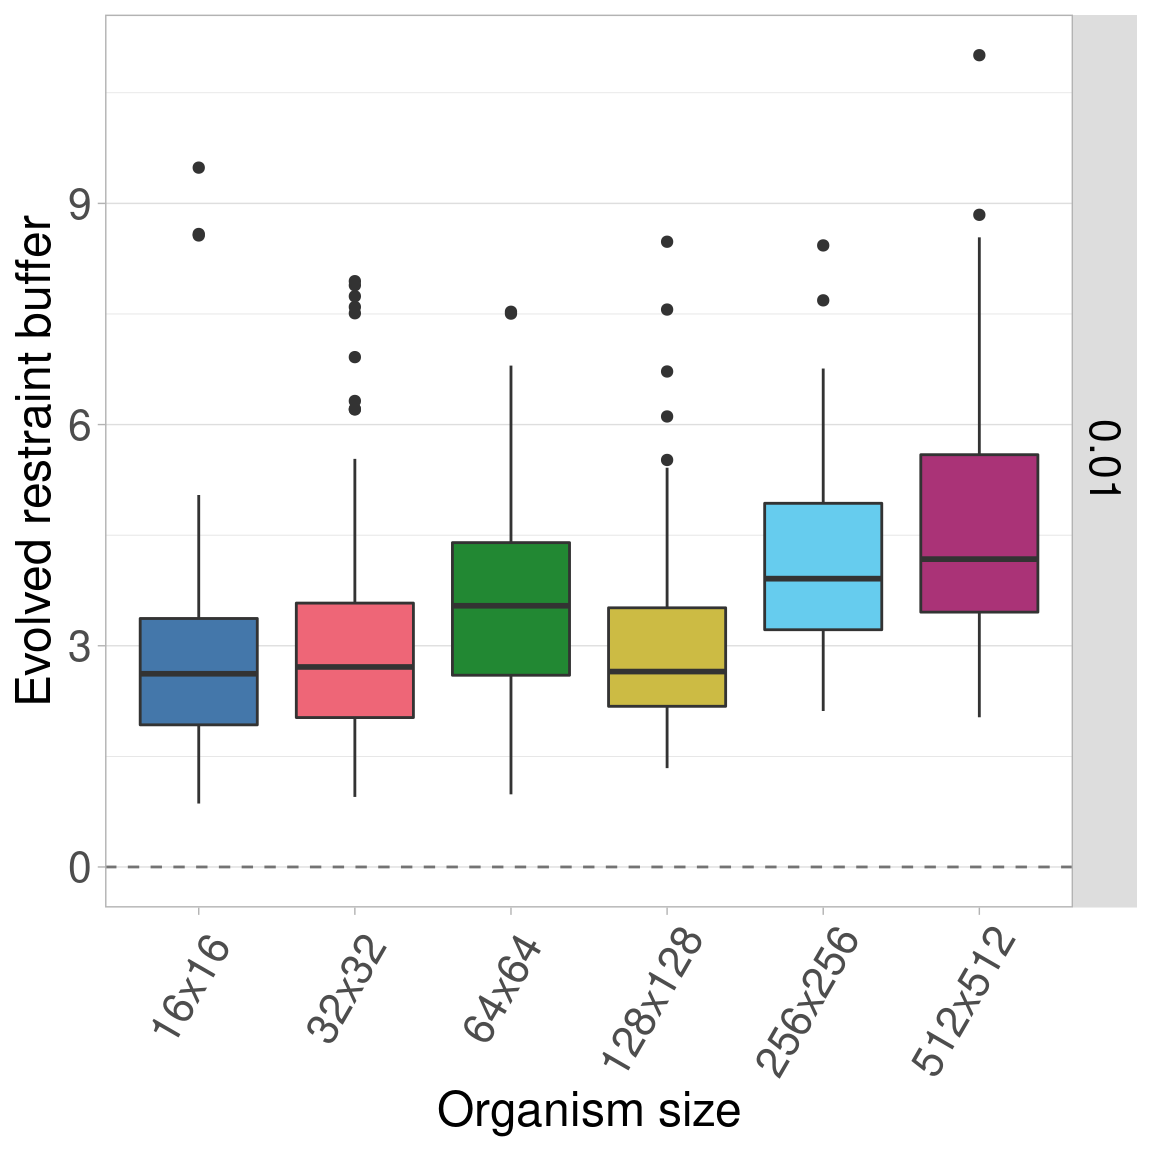
\includegraphics{primordium_supplemental_material_files/figure-latex/unnamed-chunk-25-1.pdf}

\hypertarget{somatic-mut.-rate-0.02}{%
\subsection{Somatic mut. rate 0.02}\label{somatic-mut.-rate-0.02}}

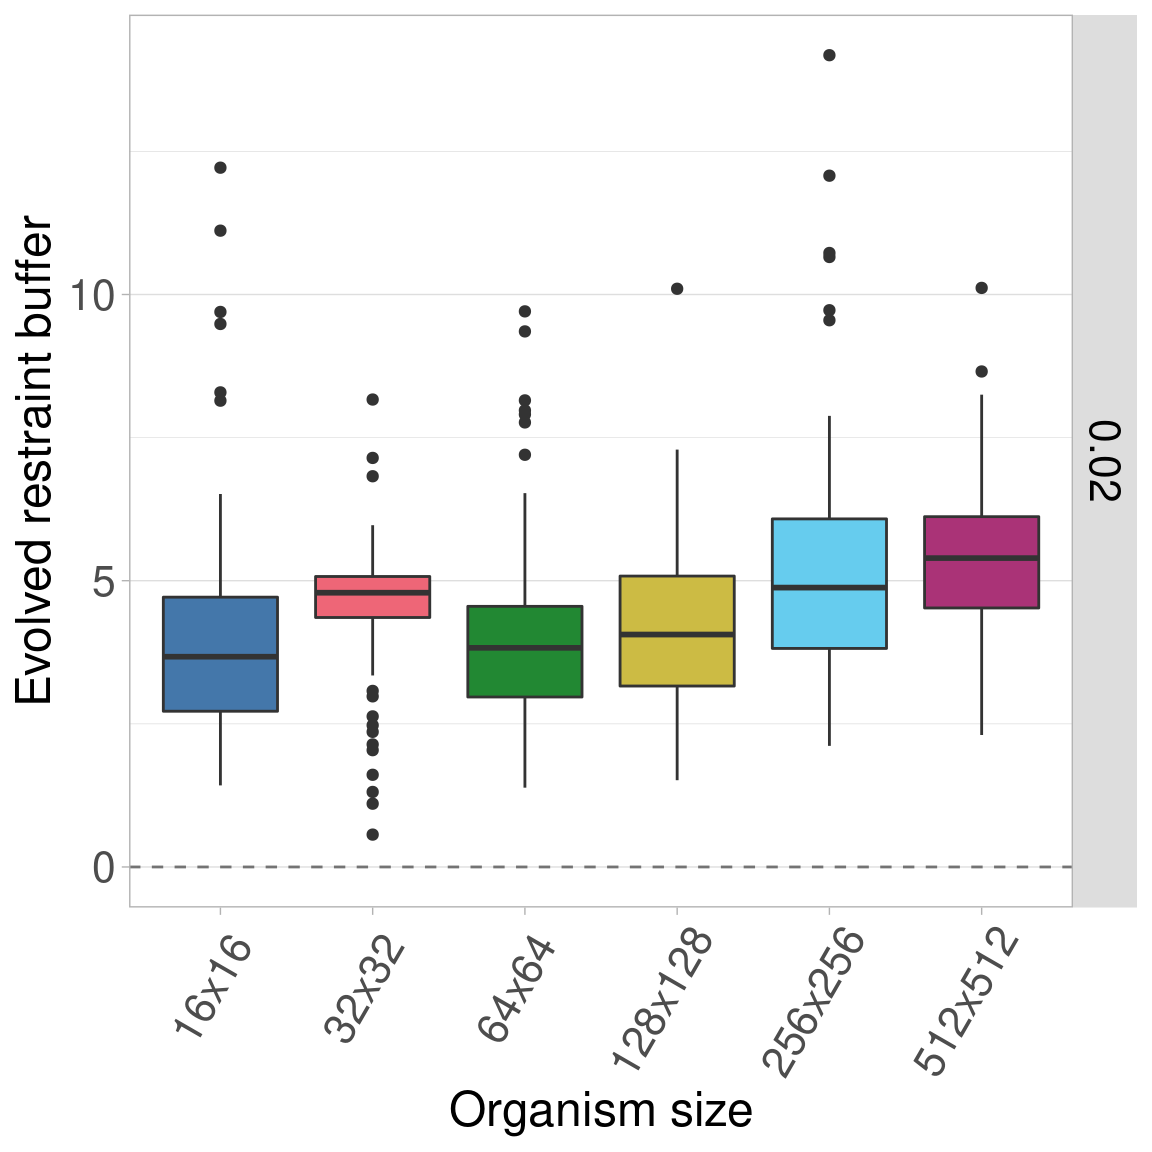
\includegraphics{primordium_supplemental_material_files/figure-latex/unnamed-chunk-26-1.pdf}

\hypertarget{somatic-mut.-rate-0.05}{%
\subsection{Somatic mut. rate 0.05}\label{somatic-mut.-rate-0.05}}

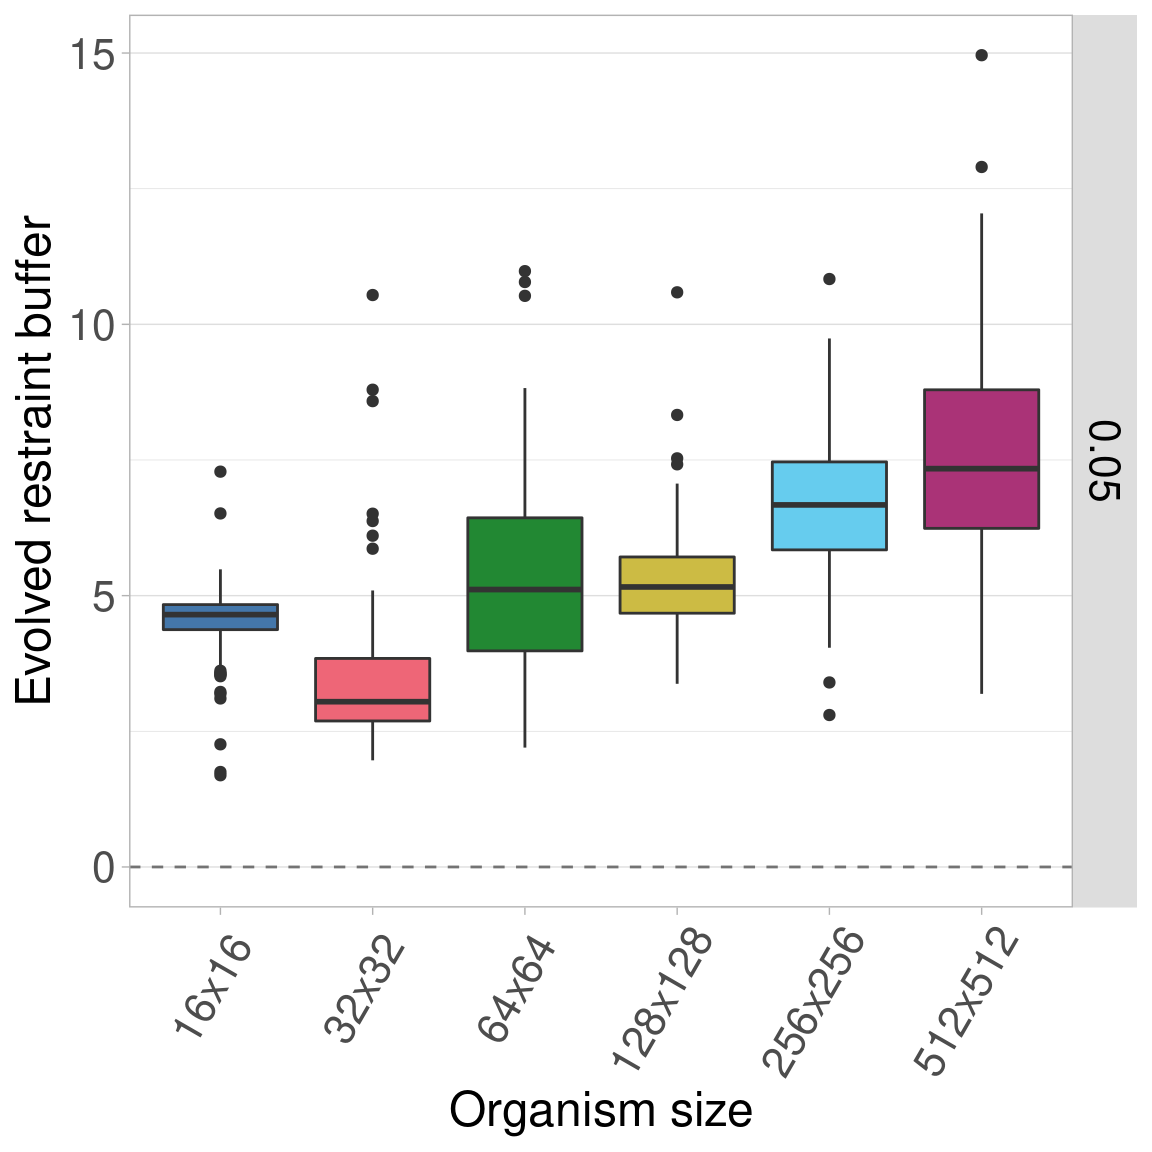
\includegraphics{primordium_supplemental_material_files/figure-latex/unnamed-chunk-27-1.pdf}

\hypertarget{somatic-mut.-rate-0.1}{%
\subsection{Somatic mut. rate 0.1}\label{somatic-mut.-rate-0.1}}

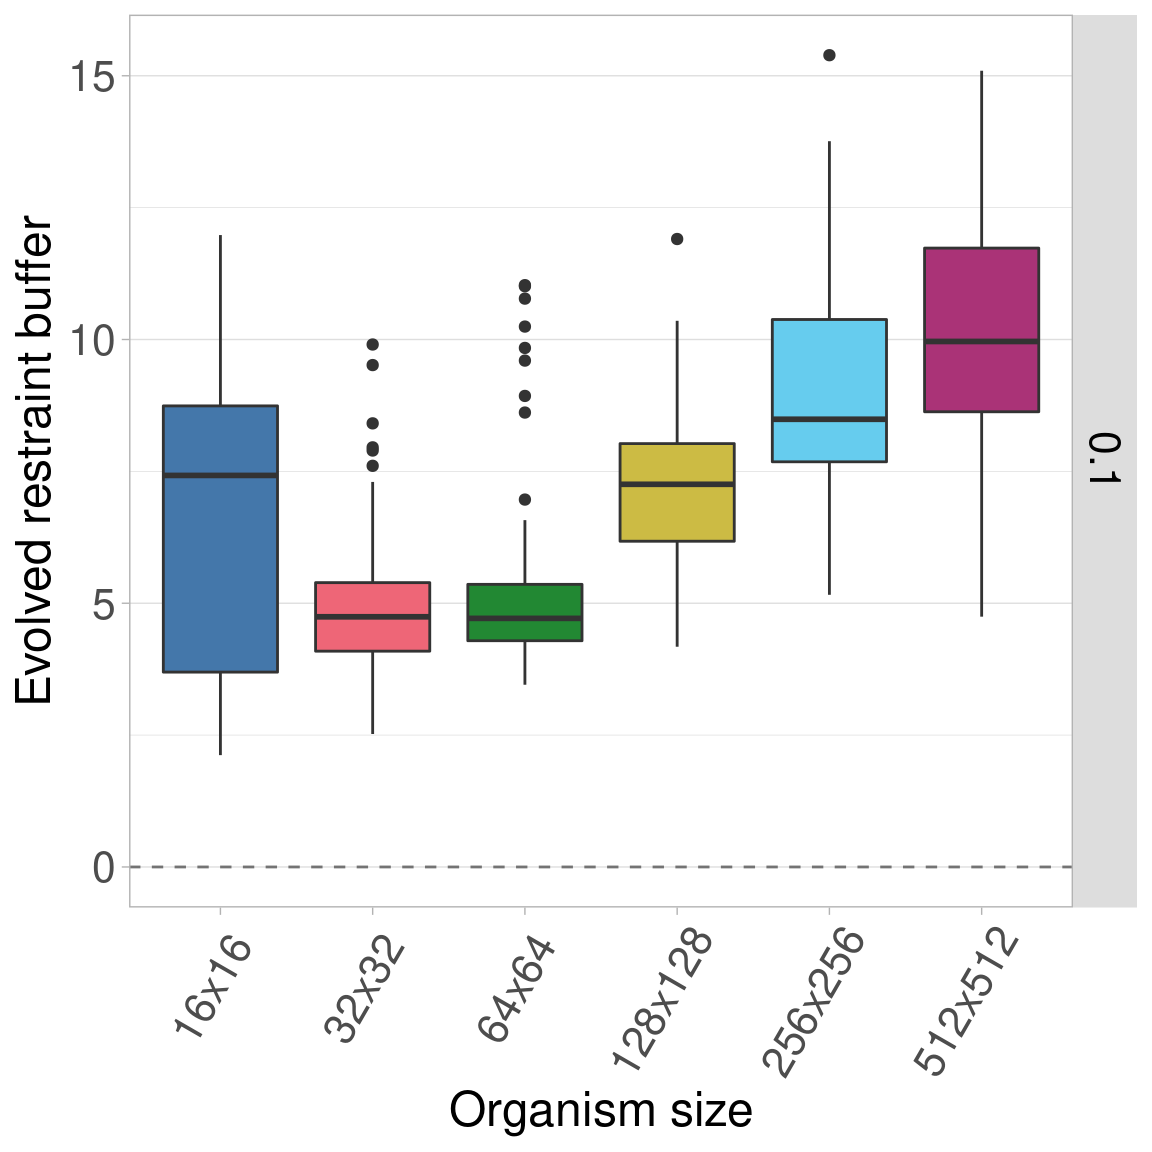
\includegraphics{primordium_supplemental_material_files/figure-latex/unnamed-chunk-28-1.pdf}

\hypertarget{somatic-mut.-rate-0.2}{%
\subsection{Somatic mut. rate 0.2}\label{somatic-mut.-rate-0.2}}

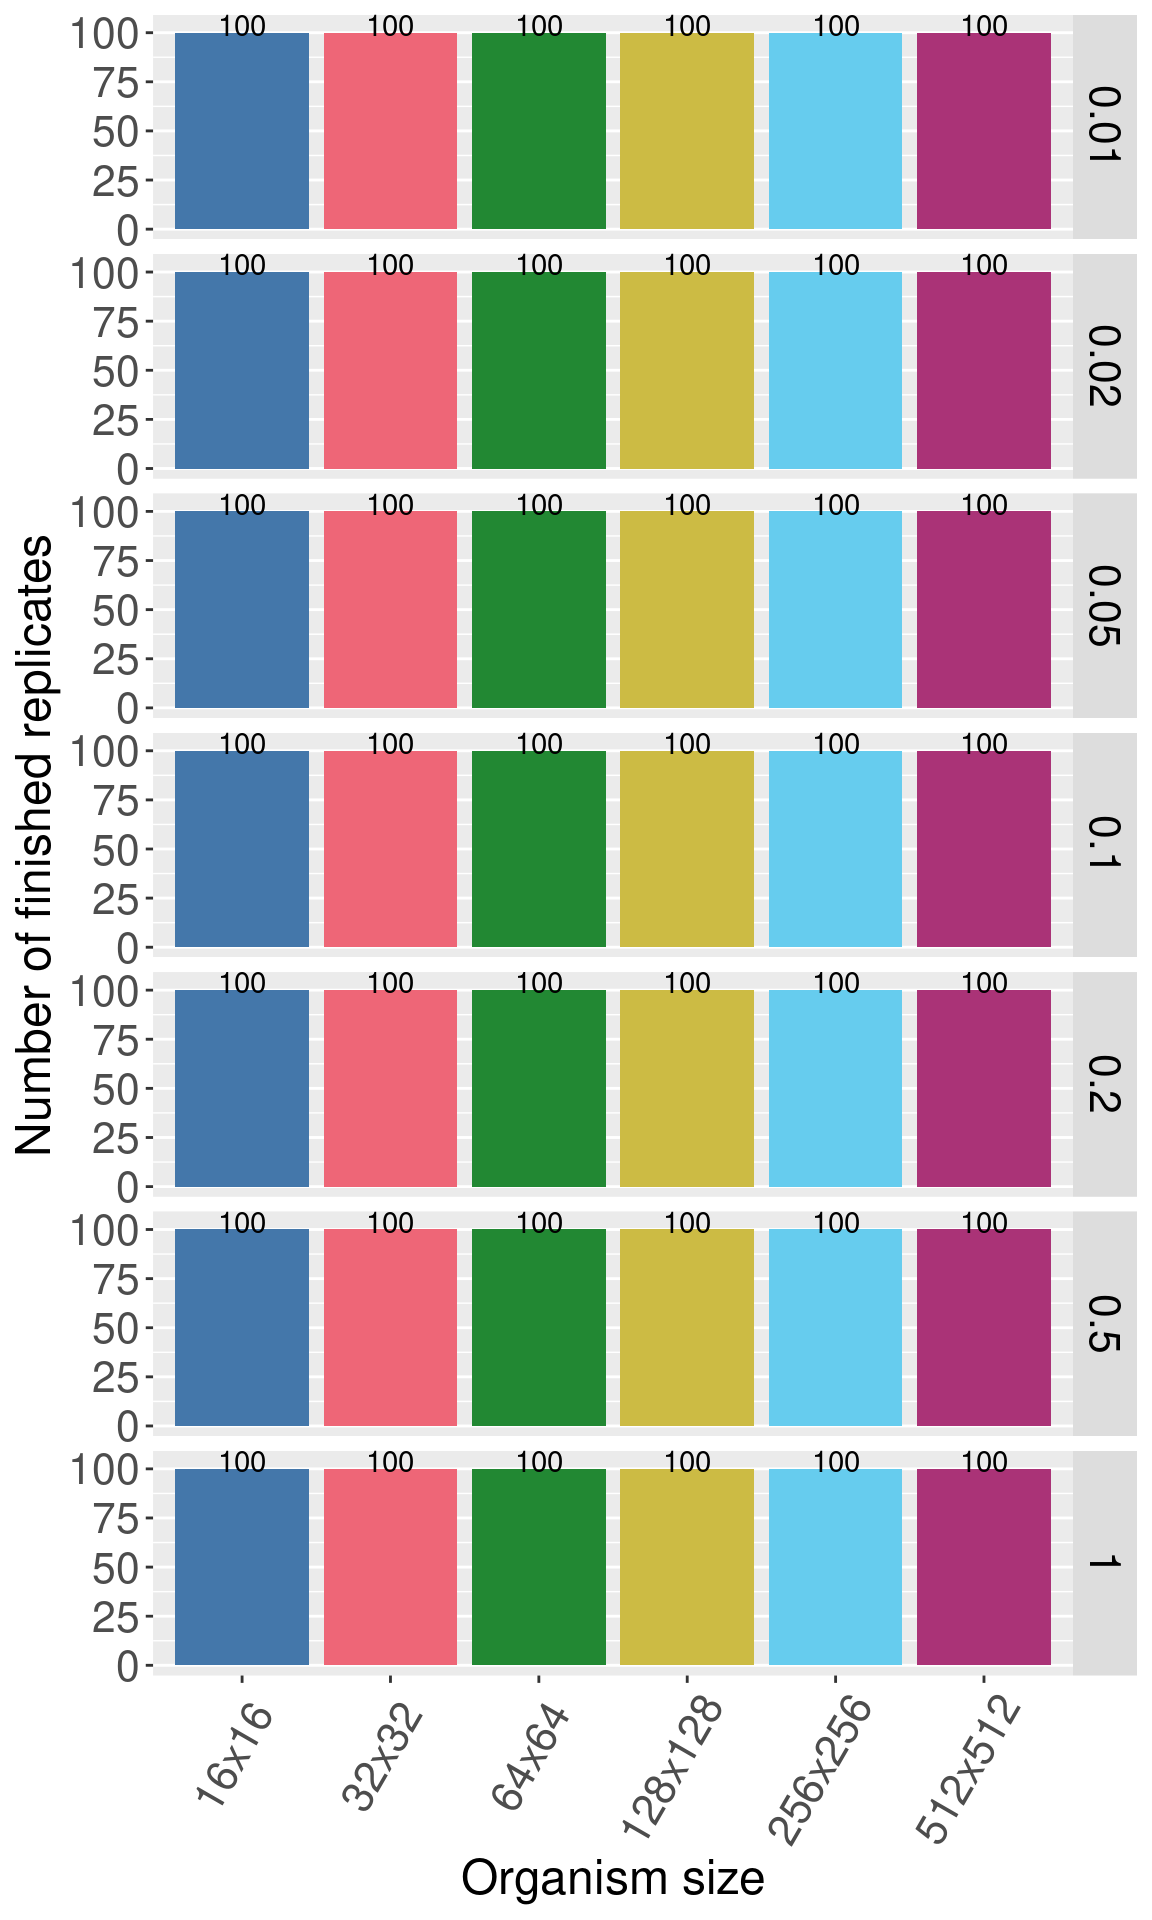
\includegraphics{primordium_supplemental_material_files/figure-latex/unnamed-chunk-29-1.pdf}

\hypertarget{somatic-mut.-rate-0.5}{%
\subsection{Somatic mut. rate 0.5}\label{somatic-mut.-rate-0.5}}

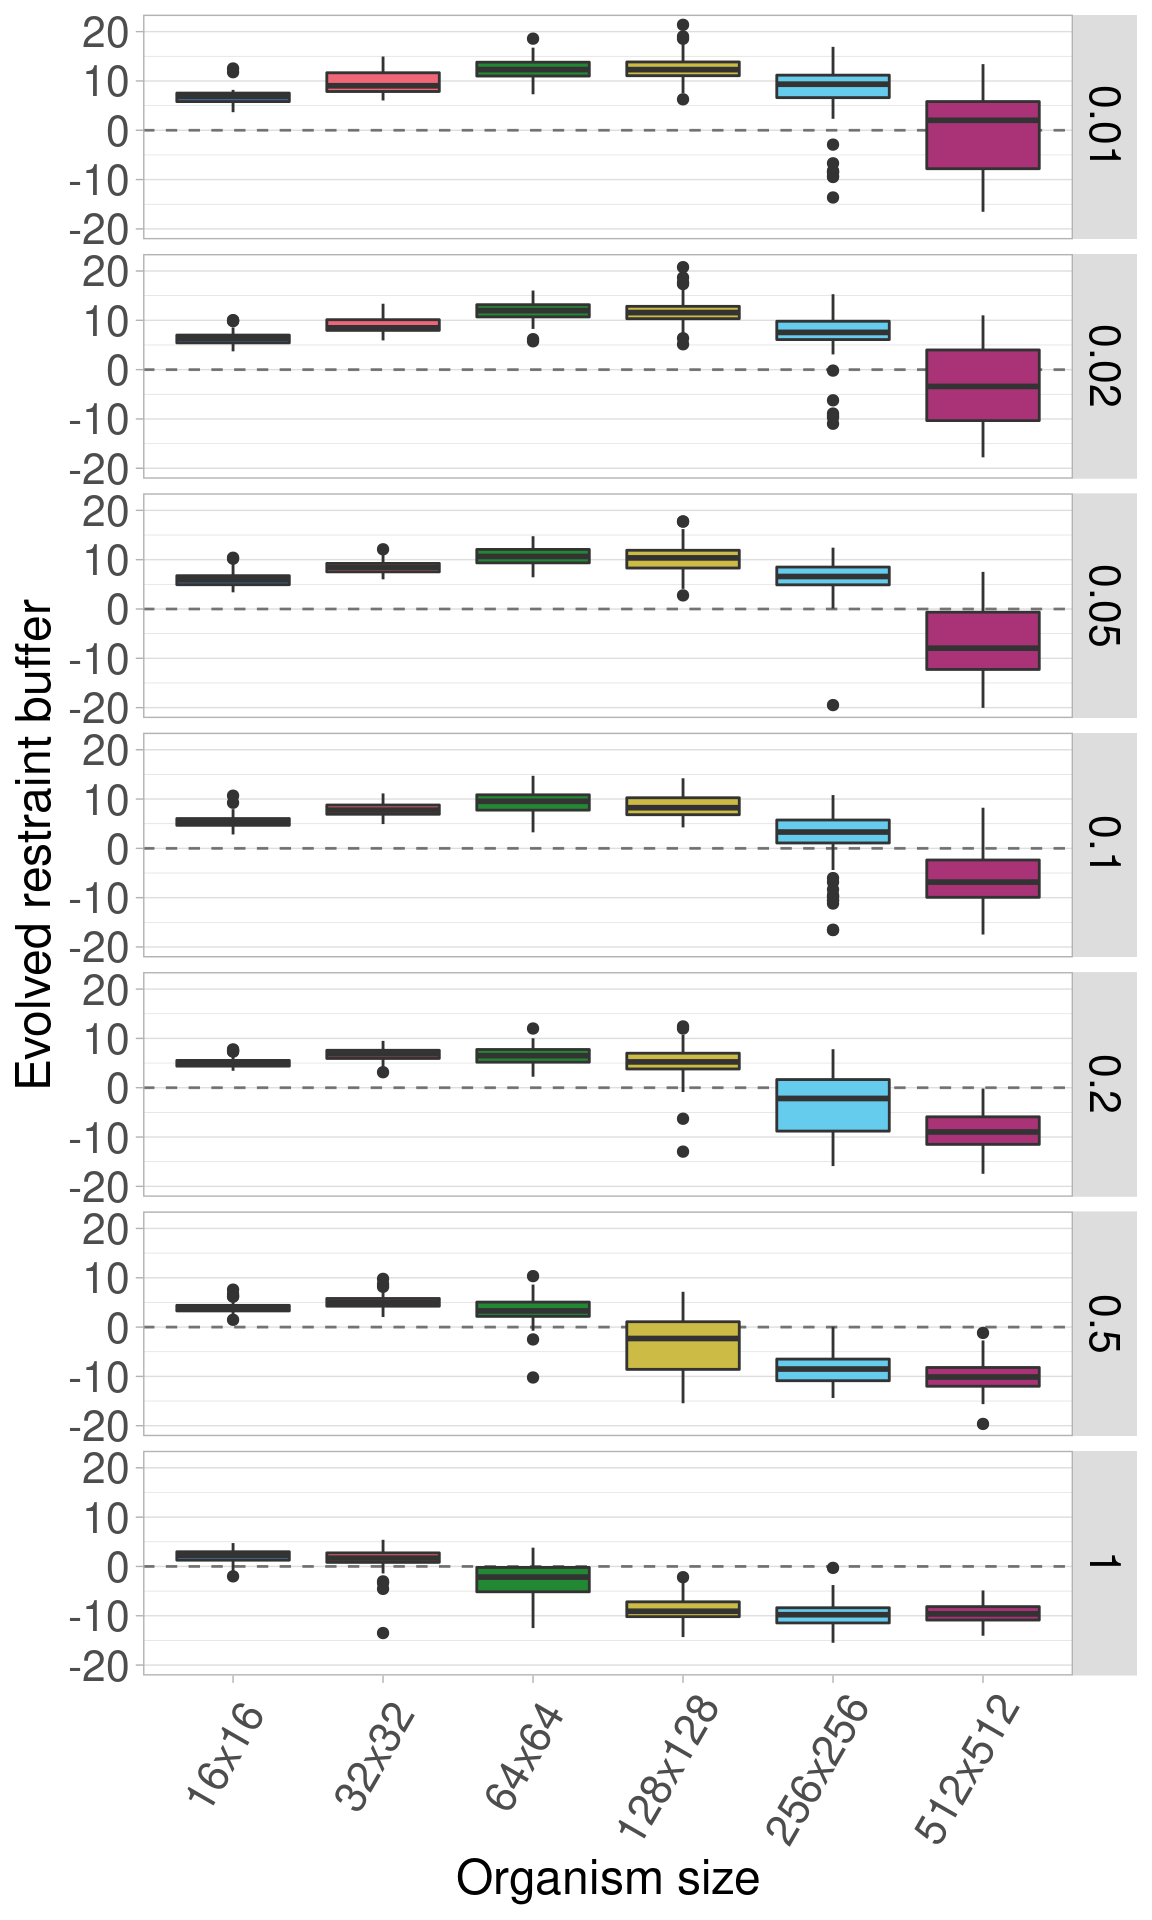
\includegraphics{primordium_supplemental_material_files/figure-latex/unnamed-chunk-30-1.pdf}

\hypertarget{somatic-mut.-rate-1.0}{%
\subsection{Somatic mut. rate 1.0}\label{somatic-mut.-rate-1.0}}

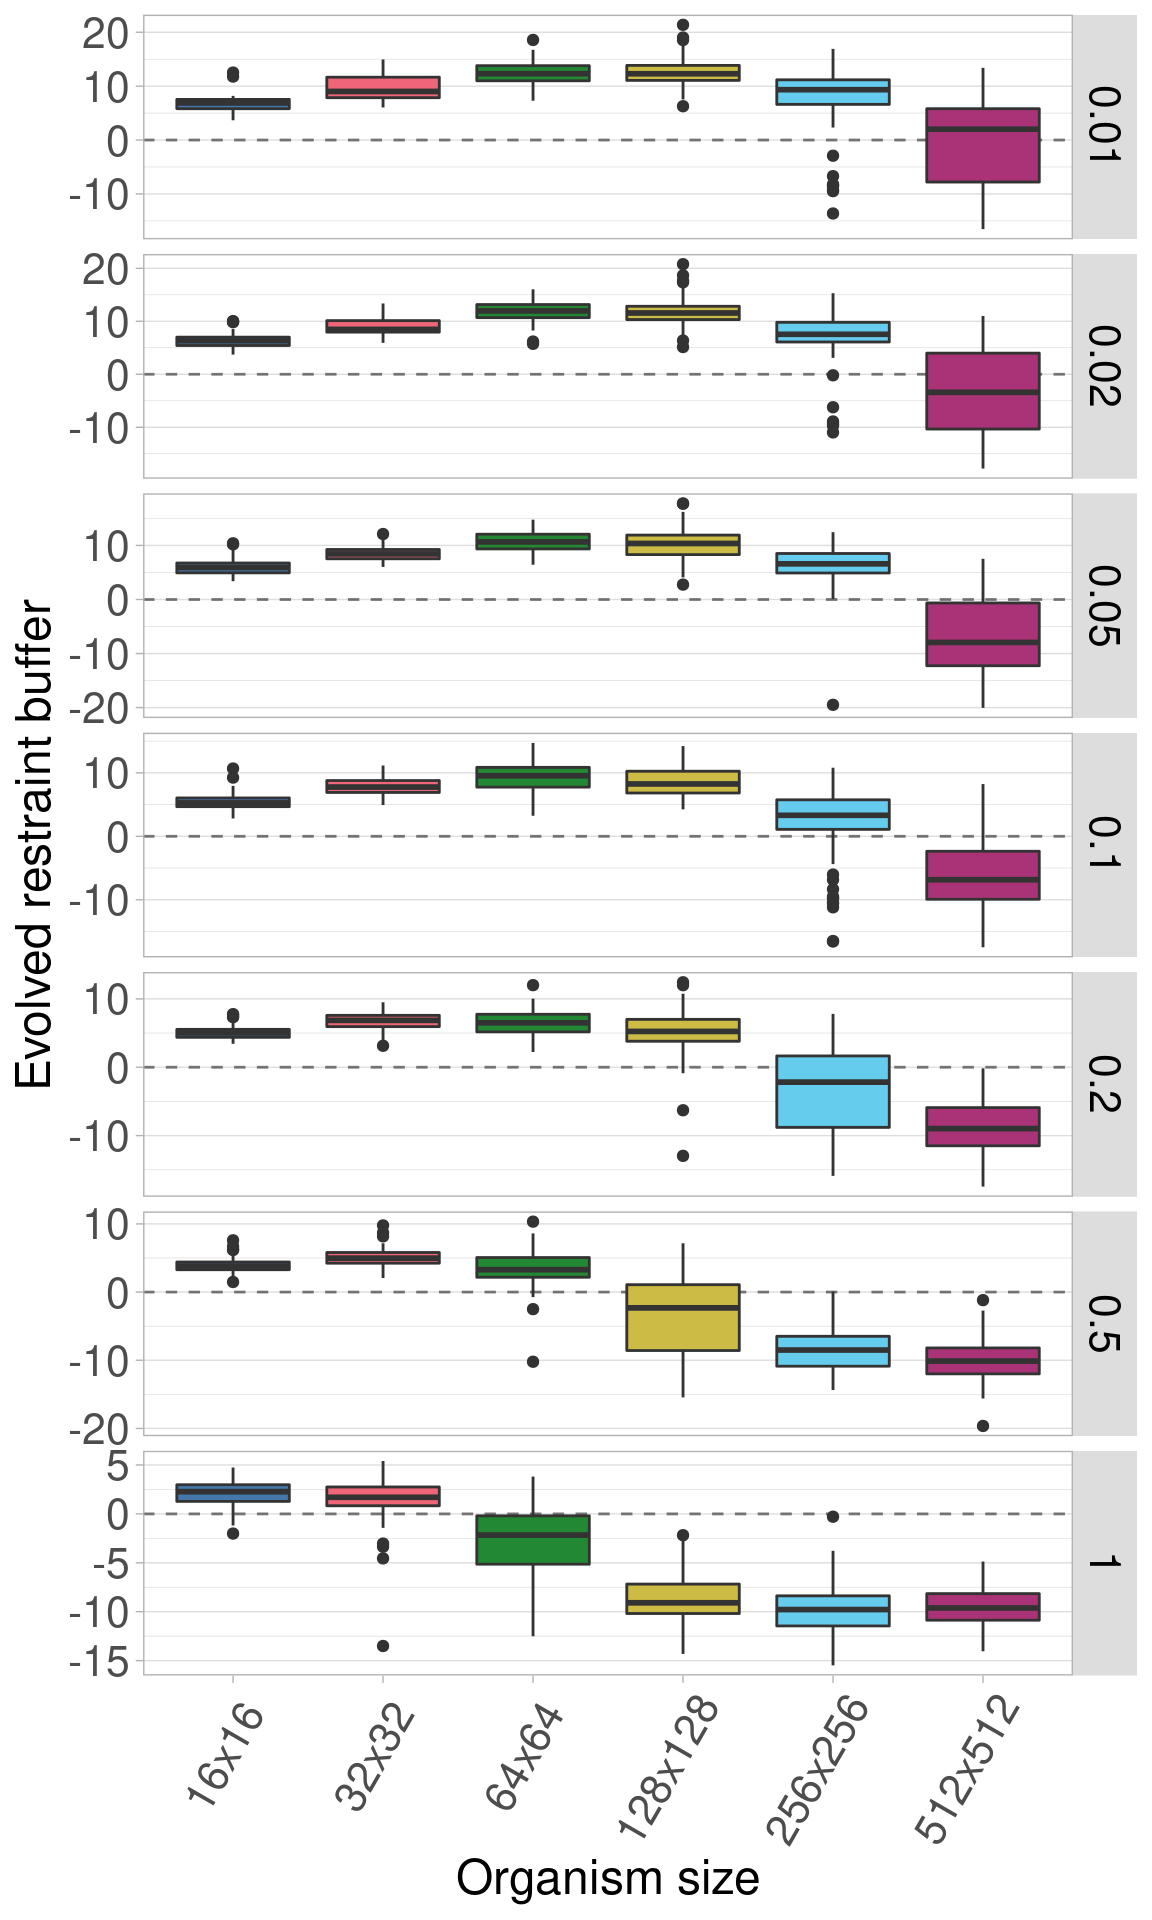
\includegraphics{primordium_supplemental_material_files/figure-latex/unnamed-chunk-31-1.pdf}

\hypertarget{statistics-1}{%
\section{Statistics}\label{statistics-1}}

Since organism size is our main point of comparison, we calculate stats for each somatic mutation rate.

First, we perform a Kruskal-Wallis test across all organism sizes to indicate if variance exists at that mutation rate.
If variance exists, we then perfrm a pairwise Wilcoxon Rank-Sum test to show which pairs of organism sizes significantly differ.
Finally, we perform Bonferroni-Holm corrections for multiple comparisons.

\begin{Shaded}
\begin{Highlighting}[]
\NormalTok{  mut_vec =}\StringTok{ }\KeywordTok{c}\NormalTok{(}\FloatTok{0.01}\NormalTok{, }\FloatTok{0.02}\NormalTok{, }\FloatTok{0.05}\NormalTok{, }\FloatTok{0.1}\NormalTok{, }\FloatTok{0.2}\NormalTok{, }\FloatTok{0.5}\NormalTok{, }\DecValTok{1}\NormalTok{)}
\NormalTok{  df_kruskal =}\StringTok{ }\KeywordTok{data.frame}\NormalTok{(}\DataTypeTok{data =} \KeywordTok{matrix}\NormalTok{(}\DataTypeTok{nrow =} \DecValTok{0}\NormalTok{, }\DataTypeTok{ncol =} \DecValTok{4}\NormalTok{))}
  \KeywordTok{colnames}\NormalTok{(df_kruskal) =}\StringTok{ }\KeywordTok{c}\NormalTok{(}\StringTok{'soma_mut_rate'}\NormalTok{, }\StringTok{'p_value'}\NormalTok{, }\StringTok{'chi_squared'}\NormalTok{, }\StringTok{'df'}\NormalTok{)}
  \ControlFlowTok{for}\NormalTok{(mut_rate }\ControlFlowTok{in}\NormalTok{ mut_vec)\{}
\NormalTok{    df_test =}\StringTok{ }\NormalTok{df2[df2}\OperatorTok{$}\NormalTok{CELLMUT }\OperatorTok{==}\StringTok{ }\NormalTok{mut_rate,]}
\NormalTok{    res =}\StringTok{ }\KeywordTok{kruskal.test}\NormalTok{(df_test}\OperatorTok{$}\NormalTok{restraint_value }\OperatorTok{~}\StringTok{ }\NormalTok{df_test}\OperatorTok{$}\NormalTok{MCSIZE, df_test)}
\NormalTok{    df_kruskal[}\KeywordTok{nrow}\NormalTok{(df_kruskal) }\OperatorTok{+}\StringTok{ }\DecValTok{1}\NormalTok{,] =}\StringTok{ }\KeywordTok{c}\NormalTok{(mut_rate, res}\OperatorTok{$}\NormalTok{p.value, }\KeywordTok{as.numeric}\NormalTok{(res}\OperatorTok{$}\NormalTok{statistic)[}\DecValTok{1}\NormalTok{], }\KeywordTok{as.numeric}\NormalTok{(res}\OperatorTok{$}\NormalTok{parameter)[}\DecValTok{1}\NormalTok{])}
\NormalTok{  \}}
\NormalTok{  df_kruskal}\OperatorTok{$}\NormalTok{less_}\FloatTok{0.01}\NormalTok{ =}\StringTok{ }\NormalTok{df_kruskal}\OperatorTok{$}\NormalTok{p_value }\OperatorTok{<}\StringTok{ }\FloatTok{0.01}
  \KeywordTok{print}\NormalTok{(df_kruskal)}
\end{Highlighting}
\end{Shaded}

\begin{verbatim}
##   soma_mut_rate      p_value chi_squared df less_0.01
## 1          0.01 2.661659e-25    125.0566  5      TRUE
## 2          0.02 4.808020e-19     95.4471  5      TRUE
## 3          0.05 1.142677e-63    304.3847  5      TRUE
## 4          0.10 3.945761e-64    306.5323  5      TRUE
## 5          0.20 4.924029e-79    375.7743  5      TRUE
## 6          0.50 5.011460e-85    403.5832  5      TRUE
## 7          1.00 5.474947e-99    468.3229  5      TRUE
\end{verbatim}

We see that significant variation exists within each mutation rate, so we perform pariwise Wilcoxon tests on each to see which pais of sizes are significantly different.

\begin{Shaded}
\begin{Highlighting}[]
\NormalTok{size_vec =}\StringTok{ }\KeywordTok{c}\NormalTok{(}\DecValTok{16}\NormalTok{, }\DecValTok{32}\NormalTok{, }\DecValTok{64}\NormalTok{, }\DecValTok{128}\NormalTok{, }\DecValTok{256}\NormalTok{, }\DecValTok{512}\NormalTok{)}
\NormalTok{mut_vec =}\StringTok{ }\KeywordTok{c}\NormalTok{(}\FloatTok{0.01}\NormalTok{, }\FloatTok{0.02}\NormalTok{, }\FloatTok{0.05}\NormalTok{, }\FloatTok{0.1}\NormalTok{, }\FloatTok{0.2}\NormalTok{, }\FloatTok{0.5}\NormalTok{, }\DecValTok{1}\NormalTok{)}
\ControlFlowTok{for}\NormalTok{(mut_rate }\ControlFlowTok{in}\NormalTok{ mut_vec)\{}
\NormalTok{  df_test =}\StringTok{ }\NormalTok{df2[df2}\OperatorTok{$}\NormalTok{CELLMUT }\OperatorTok{==}\StringTok{ }\NormalTok{mut_rate,]}
\NormalTok{  df_wilcox =}\StringTok{ }\KeywordTok{data.frame}\NormalTok{(}\DataTypeTok{data =} \KeywordTok{matrix}\NormalTok{(}\DataTypeTok{nrow =} \DecValTok{0}\NormalTok{, }\DataTypeTok{ncol =} \DecValTok{6}\NormalTok{))}
  \KeywordTok{colnames}\NormalTok{(df_wilcox) =}\StringTok{ }\KeywordTok{c}\NormalTok{(}\StringTok{'mut_rate'}\NormalTok{, }\StringTok{'size_a'}\NormalTok{, }\StringTok{'size_b'}\NormalTok{, }\StringTok{'p_value_corrected'}\NormalTok{, }\StringTok{'p_value_raw'}\NormalTok{, }\StringTok{'W'}\NormalTok{)}
  \ControlFlowTok{for}\NormalTok{(size_idx_a }\ControlFlowTok{in} \DecValTok{1}\OperatorTok{:}\NormalTok{(}\KeywordTok{length}\NormalTok{(size_vec) }\OperatorTok{-}\StringTok{ }\DecValTok{1}\NormalTok{))\{}
\NormalTok{    size_a =}\StringTok{ }\NormalTok{size_vec[size_idx_a]}
    \ControlFlowTok{for}\NormalTok{(size_idx_b }\ControlFlowTok{in}\NormalTok{ (size_idx_a }\OperatorTok{+}\StringTok{ }\DecValTok{1}\NormalTok{)}\OperatorTok{:}\KeywordTok{length}\NormalTok{(size_vec))\{}
\NormalTok{      size_b =}\StringTok{ }\NormalTok{size_vec[size_idx_b]}
\NormalTok{      res =}\StringTok{ }\KeywordTok{wilcox.test}\NormalTok{(df_test[df_test}\OperatorTok{$}\NormalTok{MCSIZE }\OperatorTok{==}\StringTok{ }\NormalTok{size_a,]}\OperatorTok{$}\NormalTok{restraint_value, df_test[df_test}\OperatorTok{$}\NormalTok{MCSIZE }\OperatorTok{==}\StringTok{ }\NormalTok{size_b,]}\OperatorTok{$}\NormalTok{restraint_value, }\DataTypeTok{alternative =} \StringTok{'two.sided'}\NormalTok{) }
\NormalTok{      df_wilcox[}\KeywordTok{nrow}\NormalTok{(df_wilcox) }\OperatorTok{+}\StringTok{ }\DecValTok{1}\NormalTok{,] =}\StringTok{ }\KeywordTok{c}\NormalTok{(mut_rate, size_a, size_b, }\DecValTok{0}\NormalTok{, res}\OperatorTok{$}\NormalTok{p.value, }\KeywordTok{as.numeric}\NormalTok{(res}\OperatorTok{$}\NormalTok{statistic)[}\DecValTok{1}\NormalTok{])}
\NormalTok{    \}}
\NormalTok{  \}}
\NormalTok{  df_wilcox}\OperatorTok{$}\NormalTok{p_value_corrected =}\StringTok{ }\KeywordTok{p.adjust}\NormalTok{(df_wilcox}\OperatorTok{$}\NormalTok{p_value_raw, }\DataTypeTok{method =} \StringTok{'holm'}\NormalTok{)}
\NormalTok{  df_wilcox}\OperatorTok{$}\NormalTok{less_}\FloatTok{0.01}\NormalTok{ =}\StringTok{ }\NormalTok{df_wilcox}\OperatorTok{$}\NormalTok{p_value_corrected }\OperatorTok{<}\StringTok{ }\FloatTok{0.01}
  \KeywordTok{print}\NormalTok{(}\KeywordTok{paste0}\NormalTok{(}\StringTok{'Somatic mutation rate: '}\NormalTok{, mut_rate))}
  \KeywordTok{print}\NormalTok{(df_wilcox)}
\NormalTok{\}}
\end{Highlighting}
\end{Shaded}

\begin{verbatim}
## [1] "Somatic mutation rate: 0.01"
##    mut_rate size_a size_b p_value_corrected  p_value_raw      W less_0.01
## 1      0.01     16     32      9.390497e-01 4.695249e-01 4703.5     FALSE
## 2      0.01     16     64      2.988154e-04 3.735192e-05 3312.0      TRUE
## 3      0.01     16    128      7.079843e-01 2.359948e-01 4514.5     FALSE
## 4      0.01     16    256      2.034819e-12 1.453442e-13 1974.5      TRUE
## 5      0.01     16    512      4.368517e-15 2.912344e-16 1653.0      TRUE
## 6      0.01     32     64      1.074876e-02 1.535537e-03 3703.0     FALSE
## 7      0.01     32    128      9.390497e-01 7.176323e-01 4851.5     FALSE
## 8      0.01     32    256      8.111610e-09 8.111610e-10 2485.5      TRUE
## 9      0.01     32    512      1.748038e-11 1.456698e-12 2102.5      TRUE
## 10     0.01     64    128      1.074876e-02 1.601365e-03 6292.0     FALSE
## 11     0.01     64    256      1.397091e-02 2.794183e-03 3776.0     FALSE
## 12     0.01     64    512      7.748038e-05 8.608931e-06 3178.5      TRUE
## 13     0.01    128    256      3.676583e-09 3.342348e-10 2428.5      TRUE
## 14     0.01    128    512      2.110112e-12 1.623163e-13 1980.5      TRUE
## 15     0.01    256    512      2.266729e-01 5.666822e-02 4219.5     FALSE
## [1] "Somatic mutation rate: 0.02"
##    mut_rate size_a size_b p_value_corrected  p_value_raw      W less_0.01
## 1      0.02     16     32      3.611494e-05 4.012771e-06 3112.5      TRUE
## 2      0.02     16     64      4.740405e-01 4.740405e-01 4706.5     FALSE
## 3      0.02     16    128      2.648393e-01 5.296786e-02 4207.5     FALSE
## 4      0.02     16    256      6.698428e-07 5.582024e-08 2776.5      TRUE
## 5      0.02     16    512      4.142268e-11 2.761512e-12 2139.0      TRUE
## 6      0.02     32     64      1.240992e-05 1.240992e-06 6985.0      TRUE
## 7      0.02     32    128      2.150816e-02 3.584693e-03 6192.5     FALSE
## 8      0.02     32    256      3.993493e-01 9.983733e-02 4326.0     FALSE
## 9      0.02     32    512      1.117168e-04 1.396459e-05 3221.5      TRUE
## 10     0.02     64    128      4.025666e-01 2.012833e-01 4476.5     FALSE
## 11     0.02     64    256      5.648464e-06 5.134967e-07 2944.5      TRUE
## 12     0.02     64    512      6.120346e-11 4.371676e-12 2165.5      TRUE
## 13     0.02    128    256      3.129242e-04 4.470345e-05 3329.0      TRUE
## 14     0.02    128    512      1.760116e-08 1.353935e-09 2519.0      TRUE
## 15     0.02    256    512      3.993493e-01 1.013587e-01 4329.0     FALSE
## [1] "Somatic mutation rate: 0.05"
##    mut_rate size_a size_b p_value_corrected  p_value_raw      W less_0.01
## 1      0.05     16     32      8.163575e-15 9.070638e-16 8290.5      TRUE
## 2      0.05     16     64      1.254683e-03 4.182276e-04 3555.5      TRUE
## 3      0.05     16    128      2.819711e-09 5.639421e-10 2462.0      TRUE
## 4      0.05     16    256      1.007639e-23 8.396990e-25  791.0      TRUE
## 5      0.05     16    512      3.169326e-24 2.437943e-25  742.5      TRUE
## 6      0.05     32     64      9.865308e-14 1.409330e-14 1850.0      TRUE
## 7      0.05     32    128      9.672216e-22 8.792924e-23  978.5      TRUE
## 8      0.05     32    256      4.456762e-26 3.183402e-27  576.5      TRUE
## 9      0.05     32    512      1.225797e-27 8.171978e-29  441.0      TRUE
## 10     0.05     64    128      9.619980e-01 9.619980e-01 4980.0     FALSE
## 11     0.05     64    256      4.409184e-09 1.102296e-09 2505.5      TRUE
## 12     0.05     64    512      1.967988e-13 3.279979e-14 1894.5      TRUE
## 13     0.05    128    256      3.061979e-14 3.827473e-15 1782.5      TRUE
## 14     0.05    128    512      4.080298e-17 4.080298e-18 1448.5      TRUE
## 15     0.05    256    512      2.648877e-03 1.324439e-03 3685.5      TRUE
## [1] "Somatic mutation rate: 0.1"
##    mut_rate size_a size_b p_value_corrected  p_value_raw      W less_0.01
## 1       0.1     16     32      3.903716e-03 9.759291e-04 6350.0      TRUE
## 2       0.1     16     64      9.815188e-02 3.271729e-02 5874.5     FALSE
## 3       0.1     16    128      6.061146e-01 3.140880e-01 4587.5     FALSE
## 4       0.1     16    256      3.278276e-08 5.463793e-09 2612.5      TRUE
## 5       0.1     16    512      9.506115e-18 1.188264e-18 1391.5      TRUE
## 6       0.1     32     64      6.061146e-01 3.030573e-01 4578.0     FALSE
## 7       0.1     32    128      8.673971e-21 8.673971e-22 1074.0      TRUE
## 8       0.1     32    256      6.950798e-29 4.964856e-30  340.0      TRUE
## 9       0.1     32    512      1.934395e-30 1.289597e-31  211.5      TRUE
## 10      0.1     64    128      2.239733e-18 2.488592e-19 1320.5      TRUE
## 11      0.1     64    256      1.194130e-25 9.951080e-27  619.5      TRUE
## 12      0.1     64    512      1.966283e-27 1.512525e-28  463.5      TRUE
## 13      0.1    128    256      8.038941e-11 1.148420e-11 2222.0      TRUE
## 14      0.1    128    512      1.880691e-21 1.709719e-22 1006.0      TRUE
## 15      0.1    256    512      3.931365e-04 7.862729e-05 3383.5      TRUE
## [1] "Somatic mutation rate: 0.2"
##    mut_rate size_a size_b p_value_corrected  p_value_raw      W less_0.01
## 1       0.2     16     32      1.077048e-02 5.385238e-03 3860.5     FALSE
## 2       0.2     16     64      6.720281e-24 8.400351e-25  791.0      TRUE
## 3       0.2     16    128      1.215721e-28 1.013101e-29  365.5      TRUE
## 4       0.2     16    256      4.359012e-29 3.353086e-30  326.0      TRUE
## 5       0.2     16    512      3.611807e-25 3.283461e-26  665.0      TRUE
## 6       0.2     32     64      5.255254e-22 7.507505e-23  972.0      TRUE
## 7       0.2     32    128      3.542154e-29 2.530110e-30  316.0      TRUE
## 8       0.2     32    256      3.153758e-30 2.102505e-31  228.5      TRUE
## 9       0.2     32    512      1.346976e-24 1.496640e-25  723.5      TRUE
## 10      0.2     64    128      1.237545e-13 2.062574e-14 1870.0      TRUE
## 11      0.2     64    256      6.129521e-25 6.129521e-26  689.0      TRUE
## 12      0.2     64    512      1.436552e-07 2.873105e-08 2728.5      TRUE
## 13      0.2    128    256      6.935985e-03 2.311995e-03 3752.5      TRUE
## 14      0.2    128    512      1.987108e-01 1.987108e-01 5526.5     FALSE
## 15      0.2    256    512      3.309684e-04 8.274210e-05 6611.5      TRUE
## [1] "Somatic mutation rate: 0.5"
##    mut_rate size_a size_b p_value_corrected  p_value_raw      W less_0.01
## 1       0.5     16     32      1.212403e-25 1.212403e-26  627.0      TRUE
## 2       0.5     16     64      1.029212e-31 7.351512e-33  113.0      TRUE
## 3       0.5     16    128      1.432034e-27 1.301849e-28  458.0      TRUE
## 4       0.5     16    256      3.887685e-06 1.295895e-06 3018.5      TRUE
## 5       0.5     16    512      1.499786e-19 2.499644e-20 8781.5      TRUE
## 6       0.5     32     64      3.854284e-24 4.282538e-25  764.5      TRUE
## 7       0.5     32    128      6.344735e-14 1.268947e-14 1844.5      TRUE
## 8       0.5     32    256      6.346151e-01 6.346151e-01 5195.0     FALSE
## 9       0.5     32    512      3.036159e-31 2.335507e-32 9847.5      TRUE
## 10      0.5     64    128      9.397051e-03 4.698526e-03 6157.5      TRUE
## 11      0.5     64    256      6.907801e-20 9.868288e-21 8822.0      TRUE
## 12      0.5     64    512      9.160009e-33 6.106673e-34 9971.0      TRUE
## 13      0.5    128    256      4.999760e-11 1.249940e-11 7773.0      TRUE
## 14      0.5    128    512      6.054856e-31 5.045714e-32 9821.0      TRUE
## 15      0.5    256    512      4.216225e-21 5.270281e-22 8947.0      TRUE
## [1] "Somatic mutation rate: 1"
##    mut_rate size_a size_b p_value_corrected  p_value_raw       W less_0.01
## 1         1     16     32      2.812620e-27 3.515774e-28   494.5      TRUE
## 2         1     16     64      5.606003e-22 9.343338e-23   981.0      TRUE
## 3         1     16    128      2.202125e-02 1.101063e-02  6041.0     FALSE
## 4         1     16    256      4.073858e-28 4.526509e-29  9580.5      TRUE
## 5         1     16    512      3.841268e-33 2.561566e-34 10000.0      TRUE
## 6         1     32     64      7.619035e-01 7.619035e-01  5124.5     FALSE
## 7         1     32    128      2.931097e-22 4.187282e-23  9052.0      TRUE
## 8         1     32    256      3.841268e-33 2.976903e-34  9995.0      TRUE
## 9         1     32    512      3.841268e-33 2.561711e-34 10000.0      TRUE
## 10        1     64    128      1.456083e-19 3.640207e-20  8765.0      TRUE
## 11        1     64    256      2.413338e-32 2.193944e-33  9928.0      TRUE
## 12        1     64    512      3.841268e-33 2.560845e-34 10000.0      TRUE
## 13        1    128    256      1.180975e-20 2.361951e-21  8883.5      TRUE
## 14        1    128    512      1.253447e-30 1.253447e-31  9789.5      TRUE
## 15        1    256    512      6.072904e-07 2.024301e-07  7127.5      TRUE
\end{verbatim}

\hypertarget{germ-mutation-rate-sweep}{%
\chapter{Germ Mutation Rate Sweep}\label{germ-mutation-rate-sweep}}

This experiment was one of the prelimary experiments we conducted to find the default parameters for Primordium.
We varied the mutation rate, the probability that an offspring experineces a mutation to its restraint buffer during organism reproduction.

The final default germ mutation rate was 0.02 (\emph{i.e.}, each organism reproduction has a 2\% chance of mutation).

The configuration script and data for the experiment can be found under \texttt{2021\_02\_16\_\_germ\_mut\_fin/} in the experiments directory of the git repository.

Load necessary libraries

\begin{Shaded}
\begin{Highlighting}[]
\KeywordTok{library}\NormalTok{(dplyr)}
\KeywordTok{library}\NormalTok{(ggplot2)}
\KeywordTok{library}\NormalTok{(ggridges)}
\KeywordTok{library}\NormalTok{(scales)}
\KeywordTok{library}\NormalTok{(khroma)}
\end{Highlighting}
\end{Shaded}

Load the data and trim all the unecessay bits (\emph{e.g.}, we initially ran sizes 8x8, 1024x1024 but cut them from the paper to make plots easier to read).

\begin{Shaded}
\begin{Highlighting}[]
\CommentTok{# Load the data}
\NormalTok{df =}\StringTok{ }\KeywordTok{read.csv}\NormalTok{(}\StringTok{'../experiments/2021_02_16__germ_mut_fin/evolution/data/scraped_evolution_data.csv'}\NormalTok{)}
\CommentTok{#df = read.csv('/research/rogue_cell/Primordium/experiments/2021_02_16__germ_mut_fin/evolution/data/scraped_evolution_data.csv')}
\CommentTok{# Trim off NAs (artifiacts of how we scraped the data) and trim to only have gen 10,000}
\KeywordTok{cat}\NormalTok{(}\KeywordTok{colnames}\NormalTok{(df), }\StringTok{'}\CharTok{\textbackslash{}n}\StringTok{'}\NormalTok{)}
\end{Highlighting}
\end{Shaded}

\begin{verbatim}
## X generation ave_ones ave_repro_time min_ones max_ones var_ones rep_id MCSIZE COST GENS MUT POP SAMPLES REPS ONES CELLMUT
\end{verbatim}

\begin{Shaded}
\begin{Highlighting}[]
\NormalTok{df2 =}\StringTok{ }\NormalTok{df[}\OperatorTok{!}\KeywordTok{is.na}\NormalTok{(df}\OperatorTok{$}\NormalTok{MCSIZE) }\OperatorTok{&}\StringTok{ }\NormalTok{df}\OperatorTok{$}\NormalTok{generation }\OperatorTok{==}\StringTok{ }\DecValTok{10000}\NormalTok{,]}
\CommentTok{# Ignore data for size 8x8 and 1024x1024}
\NormalTok{df2 =}\StringTok{ }\NormalTok{df2[df2}\OperatorTok{$}\NormalTok{MCSIZE }\OperatorTok{!=}\StringTok{ }\DecValTok{8} \OperatorTok{&}\StringTok{ }\NormalTok{df2}\OperatorTok{$}\NormalTok{MCSIZE }\OperatorTok{!=}\StringTok{ }\DecValTok{1024}\NormalTok{,]}
\end{Highlighting}
\end{Shaded}

We group and summarize the data to make to ensure all replicates are present.

\begin{Shaded}
\begin{Highlighting}[]
\CommentTok{# Group the data by size and summarize}
\NormalTok{data_grouped =}\StringTok{ }\NormalTok{dplyr}\OperatorTok{::}\KeywordTok{group_by}\NormalTok{(df2, MCSIZE, MUT)}
\NormalTok{data_summary =}\StringTok{ }\NormalTok{dplyr}\OperatorTok{::}\KeywordTok{summarize}\NormalTok{(data_grouped, }\DataTypeTok{mean_ones =} \KeywordTok{mean}\NormalTok{(ave_ones), }\DataTypeTok{n =}\NormalTok{ dplyr}\OperatorTok{::}\KeywordTok{n}\NormalTok{())}
\end{Highlighting}
\end{Shaded}

Further cleaning of the data plus adding some variables to make plotting easier.

\begin{Shaded}
\begin{Highlighting}[]
\CommentTok{# Calculate restraint value (x - 60 because genome length is 100 here)}
\NormalTok{df2}\OperatorTok{$}\NormalTok{restraint_value =}\StringTok{ }\NormalTok{df2}\OperatorTok{$}\NormalTok{ave_ones }\OperatorTok{-}\StringTok{ }\DecValTok{60}
\CommentTok{# Make a nice, clean factor for size}
\NormalTok{df2}\OperatorTok{$}\NormalTok{size_str =}\StringTok{ }\KeywordTok{paste0}\NormalTok{(df2}\OperatorTok{$}\NormalTok{MCSIZE, }\StringTok{'x'}\NormalTok{, df2}\OperatorTok{$}\NormalTok{MCSIZE)}
\NormalTok{df2}\OperatorTok{$}\NormalTok{size_factor =}\StringTok{ }\KeywordTok{factor}\NormalTok{(df2}\OperatorTok{$}\NormalTok{size_str, }\DataTypeTok{levels =} \KeywordTok{c}\NormalTok{(}\StringTok{'16x16'}\NormalTok{, }\StringTok{'32x32'}\NormalTok{, }\StringTok{'64x64'}\NormalTok{, }\StringTok{'128x128'}\NormalTok{, }\StringTok{'256x256'}\NormalTok{, }\StringTok{'512x512'}\NormalTok{, }\StringTok{'1024x1024'}\NormalTok{))}
\NormalTok{df2}\OperatorTok{$}\NormalTok{size_factor_reversed =}\StringTok{ }\KeywordTok{factor}\NormalTok{(df2}\OperatorTok{$}\NormalTok{size_str, }\DataTypeTok{levels =} \KeywordTok{rev}\NormalTok{(}\KeywordTok{c}\NormalTok{(}\StringTok{'16x16'}\NormalTok{, }\StringTok{'32x32'}\NormalTok{, }\StringTok{'64x64'}\NormalTok{, }\StringTok{'128x128'}\NormalTok{, }\StringTok{'256x256'}\NormalTok{, }\StringTok{'512x512'}\NormalTok{, }\StringTok{'1024x1024'}\NormalTok{)))}
\NormalTok{df2}\OperatorTok{$}\NormalTok{germ_mut_str =}\StringTok{ }\KeywordTok{paste}\NormalTok{(}\StringTok{'GERM MUT'}\NormalTok{, df2}\OperatorTok{$}\NormalTok{MUT)}
\NormalTok{df2}\OperatorTok{$}\NormalTok{mut_factor =}\StringTok{ }\KeywordTok{factor}\NormalTok{(df2}\OperatorTok{$}\NormalTok{MUT, }\DataTypeTok{levels =} \KeywordTok{c}\NormalTok{(}\FloatTok{0.01}\NormalTok{, }\FloatTok{0.02}\NormalTok{, }\FloatTok{0.05}\NormalTok{, }\FloatTok{0.10}\NormalTok{, }\FloatTok{0.20}\NormalTok{, }\FloatTok{0.50}\NormalTok{, }\FloatTok{1.00}\NormalTok{))}
\NormalTok{data_summary}\OperatorTok{$}\NormalTok{size_str =}\StringTok{ }\KeywordTok{paste0}\NormalTok{(data_summary}\OperatorTok{$}\NormalTok{MCSIZE, }\StringTok{'x'}\NormalTok{, data_summary}\OperatorTok{$}\NormalTok{MCSIZE)}
\NormalTok{data_summary}\OperatorTok{$}\NormalTok{size_factor =}\StringTok{ }\KeywordTok{factor}\NormalTok{(data_summary}\OperatorTok{$}\NormalTok{size_str, }\DataTypeTok{levels =} \KeywordTok{c}\NormalTok{(}\StringTok{'16x16'}\NormalTok{, }\StringTok{'32x32'}\NormalTok{, }\StringTok{'64x64'}\NormalTok{, }\StringTok{'128x128'}\NormalTok{, }\StringTok{'256x256'}\NormalTok{, }\StringTok{'512x512'}\NormalTok{, }\StringTok{'1024x1024'}\NormalTok{))}
\NormalTok{data_summary}\OperatorTok{$}\NormalTok{germ_mut_str =}\StringTok{ }\KeywordTok{paste}\NormalTok{(}\StringTok{'GERM MUT'}\NormalTok{, data_summary}\OperatorTok{$}\NormalTok{MUT)}
\NormalTok{data_summary}\OperatorTok{$}\NormalTok{mut_factor =}\StringTok{ }\KeywordTok{factor}\NormalTok{(data_summary}\OperatorTok{$}\NormalTok{MUT, }\DataTypeTok{levels =} \KeywordTok{c}\NormalTok{(}\FloatTok{0.01}\NormalTok{, }\FloatTok{0.02}\NormalTok{, }\FloatTok{0.05}\NormalTok{, }\FloatTok{0.10}\NormalTok{, }\FloatTok{0.20}\NormalTok{, }\FloatTok{0.50}\NormalTok{, }\FloatTok{1.00}\NormalTok{))}
\CommentTok{# Create a map of colors we'll use to plot the different organism sizes}
\NormalTok{color_vec =}\StringTok{ }\KeywordTok{as.character}\NormalTok{(khroma}\OperatorTok{::}\KeywordTok{color}\NormalTok{(}\StringTok{'bright'}\NormalTok{)(}\DecValTok{7}\NormalTok{))}
\NormalTok{color_map =}\StringTok{ }\KeywordTok{c}\NormalTok{(}
  \StringTok{'16x16'}\NormalTok{ =}\StringTok{     }\NormalTok{color_vec[}\DecValTok{1}\NormalTok{],}
  \StringTok{'32x32'}\NormalTok{ =}\StringTok{     }\NormalTok{color_vec[}\DecValTok{2}\NormalTok{],}
  \StringTok{'64x64'}\NormalTok{ =}\StringTok{     }\NormalTok{color_vec[}\DecValTok{3}\NormalTok{],}
  \StringTok{'128x128'}\NormalTok{ =}\StringTok{   }\NormalTok{color_vec[}\DecValTok{4}\NormalTok{],}
  \StringTok{'256x256'}\NormalTok{ =}\StringTok{   }\NormalTok{color_vec[}\DecValTok{5}\NormalTok{],}
  \StringTok{'512x512'}\NormalTok{ =}\StringTok{   }\NormalTok{color_vec[}\DecValTok{6}\NormalTok{],}
  \StringTok{'1024x1024'}\NormalTok{ =}\StringTok{ }\NormalTok{color_vec[}\DecValTok{7}\NormalTok{]}
\NormalTok{)}
\CommentTok{# Set the sizes for text in plots}
\NormalTok{text_major_size =}\StringTok{ }\DecValTok{18}
\NormalTok{text_minor_size =}\StringTok{ }\DecValTok{16} 
\NormalTok{boxplot_color =}\StringTok{ '#9ecae1'}
\end{Highlighting}
\end{Shaded}

\hypertarget{data-integrity-check-2}{%
\section{Data integrity check}\label{data-integrity-check-2}}

Now we plot the number of finished replicates for each treatment to make sure all data are present.
Each row shows a different germ mutation rate.
Each bar/color shows a different organism size.
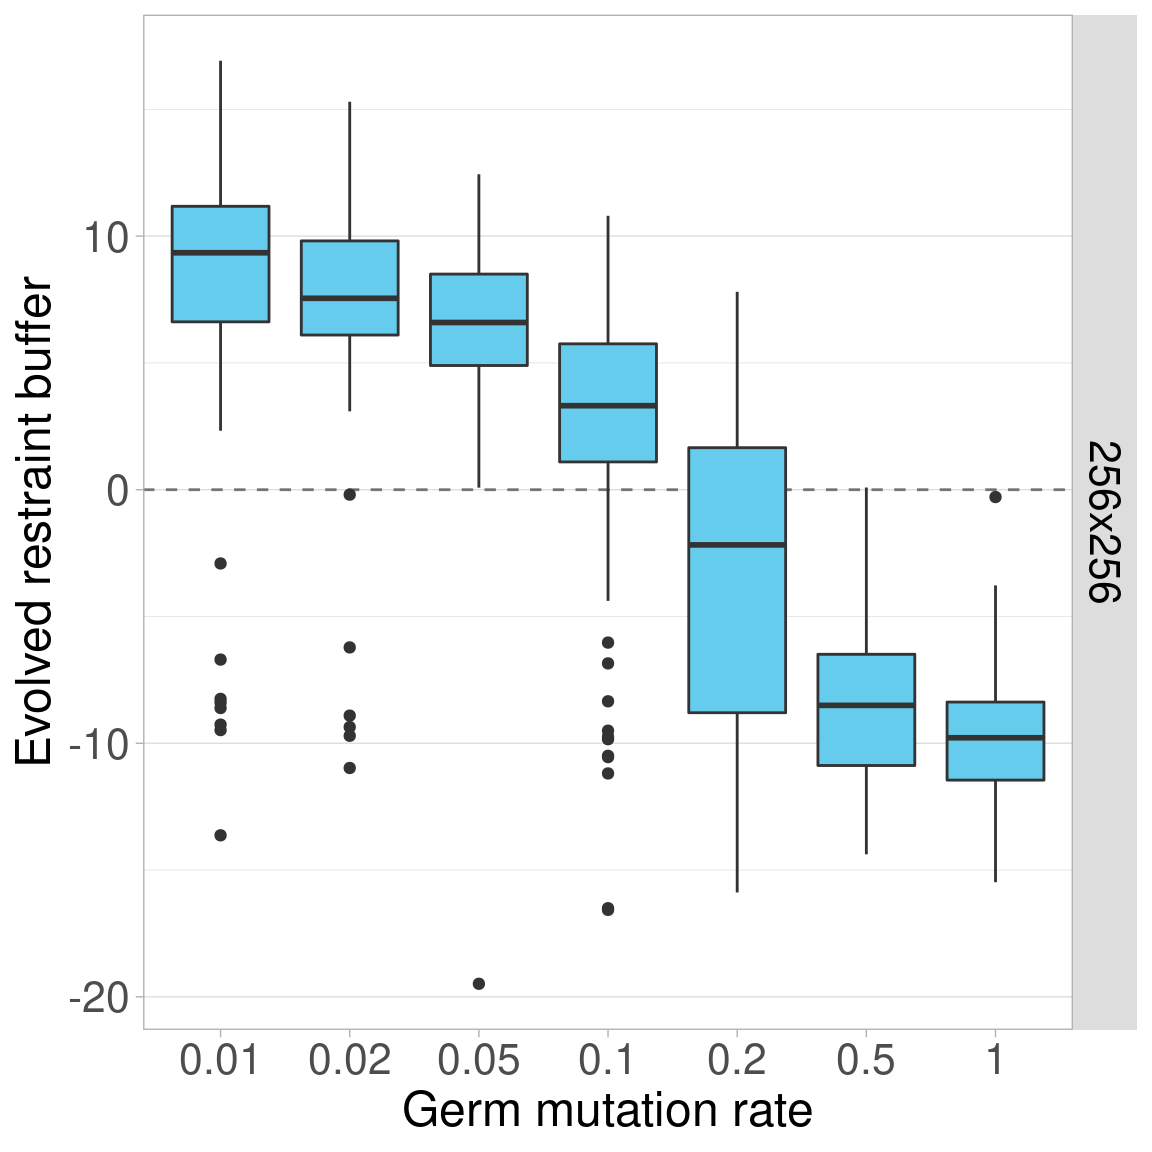
\includegraphics{primordium_supplemental_material_files/figure-latex/unnamed-chunk-38-1.pdf}

\hypertarget{aggregate-plots-2}{%
\section{Aggregate plots}\label{aggregate-plots-2}}

\hypertarget{facet-by-germ-mutation-rate}{%
\subsection{Facet by germ mutation rate}\label{facet-by-germ-mutation-rate}}

Here we plot all the data at once.
Each row shows a different germ mutation rate and each boxplot shows a given organism size.

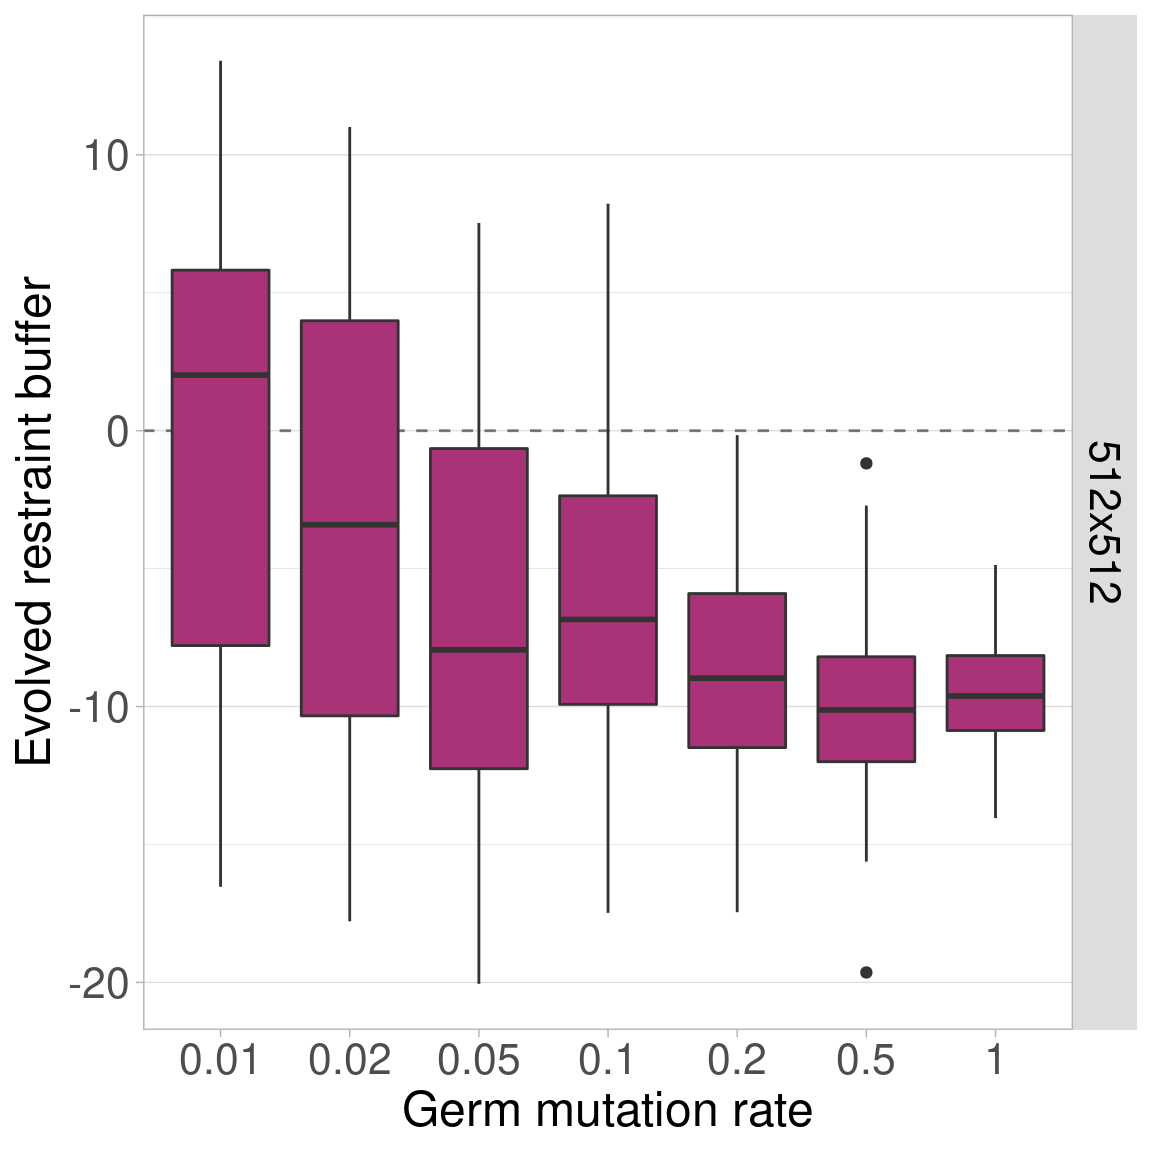
\includegraphics{primordium_supplemental_material_files/figure-latex/unnamed-chunk-39-1.pdf}

Here is the same data, plotted identically other than now each row can have a different y-axis.

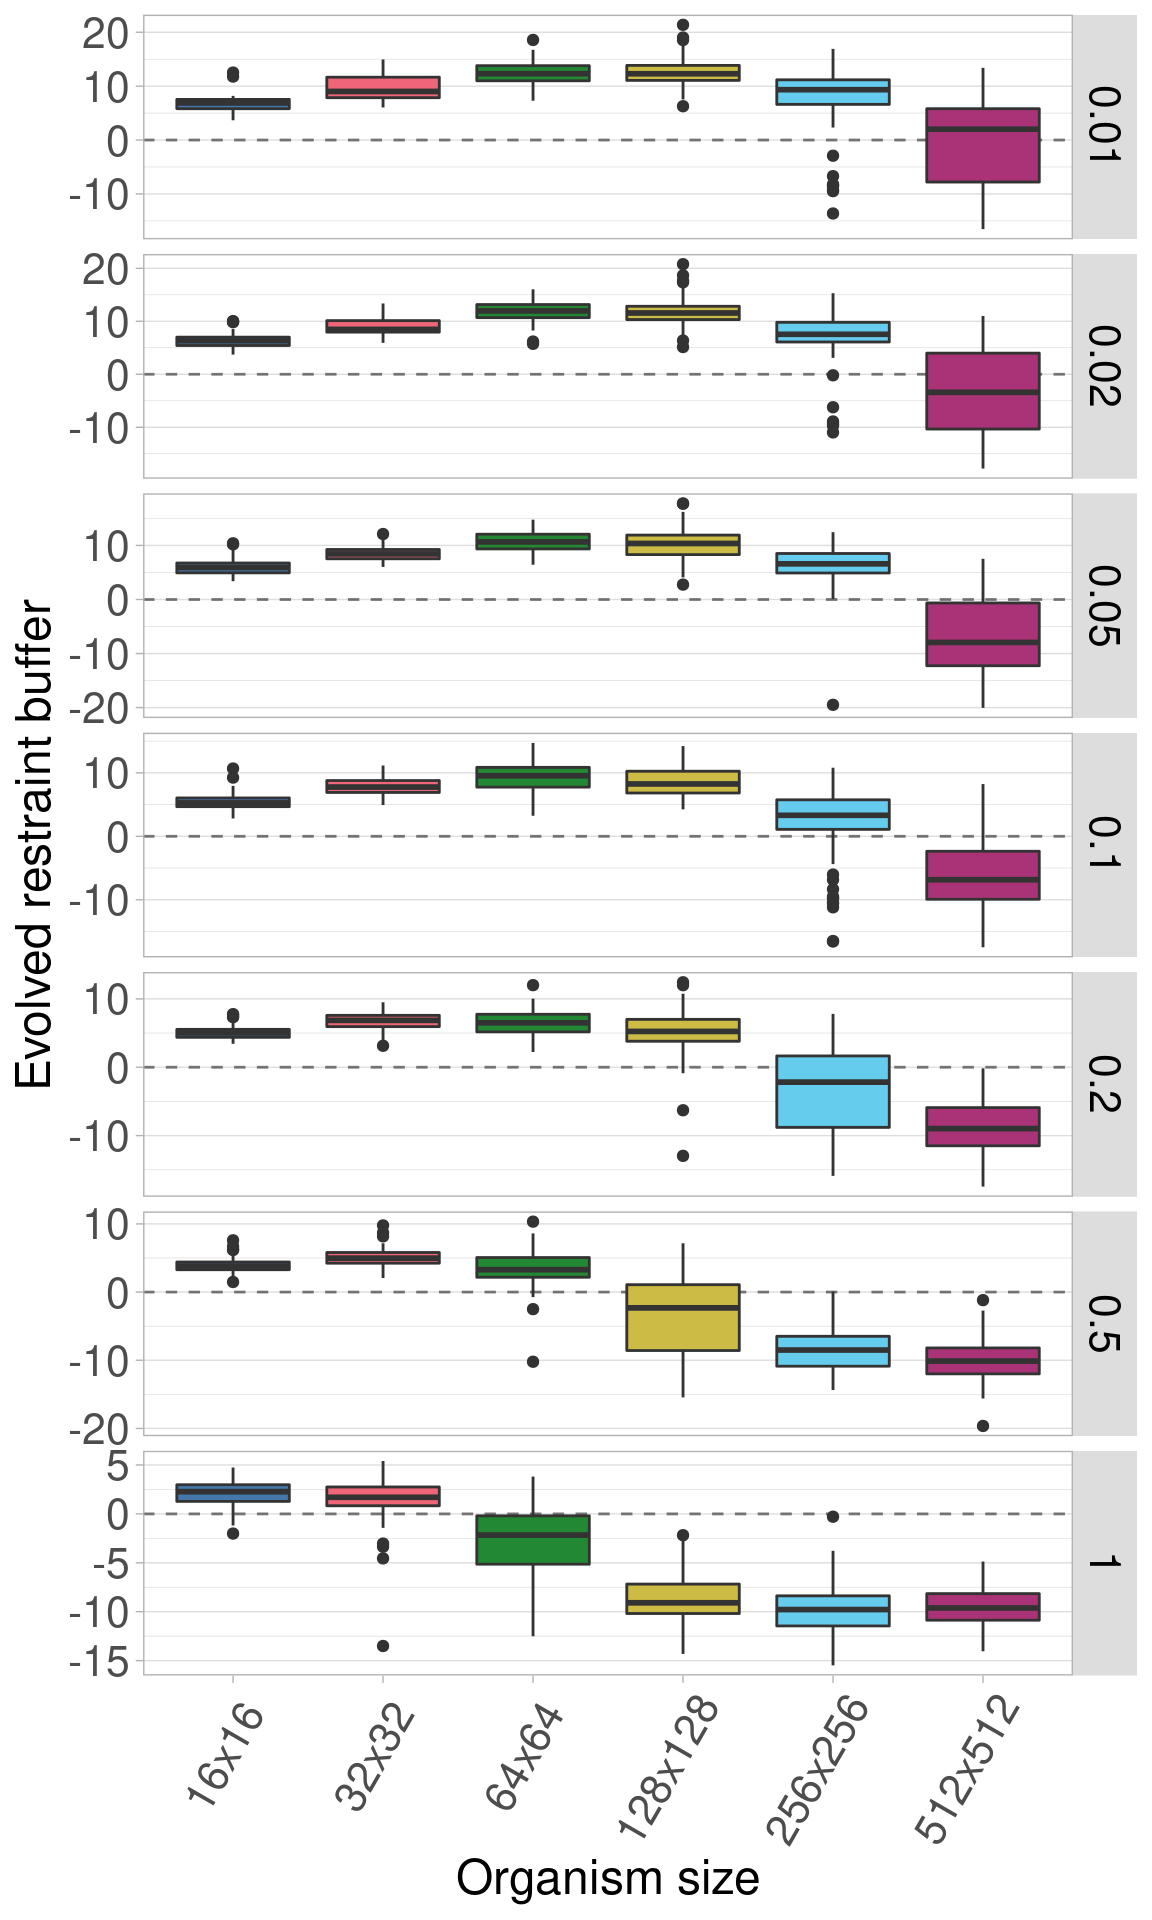
\includegraphics{primordium_supplemental_material_files/figure-latex/unnamed-chunk-40-1.pdf}

\hypertarget{facet-by-organism-size-1}{%
\subsection{Facet by organism size}\label{facet-by-organism-size-1}}

Next, we plot the same data, but this time each row corresponds to a certain organism size while germ mutation rate varies along the x-axis.

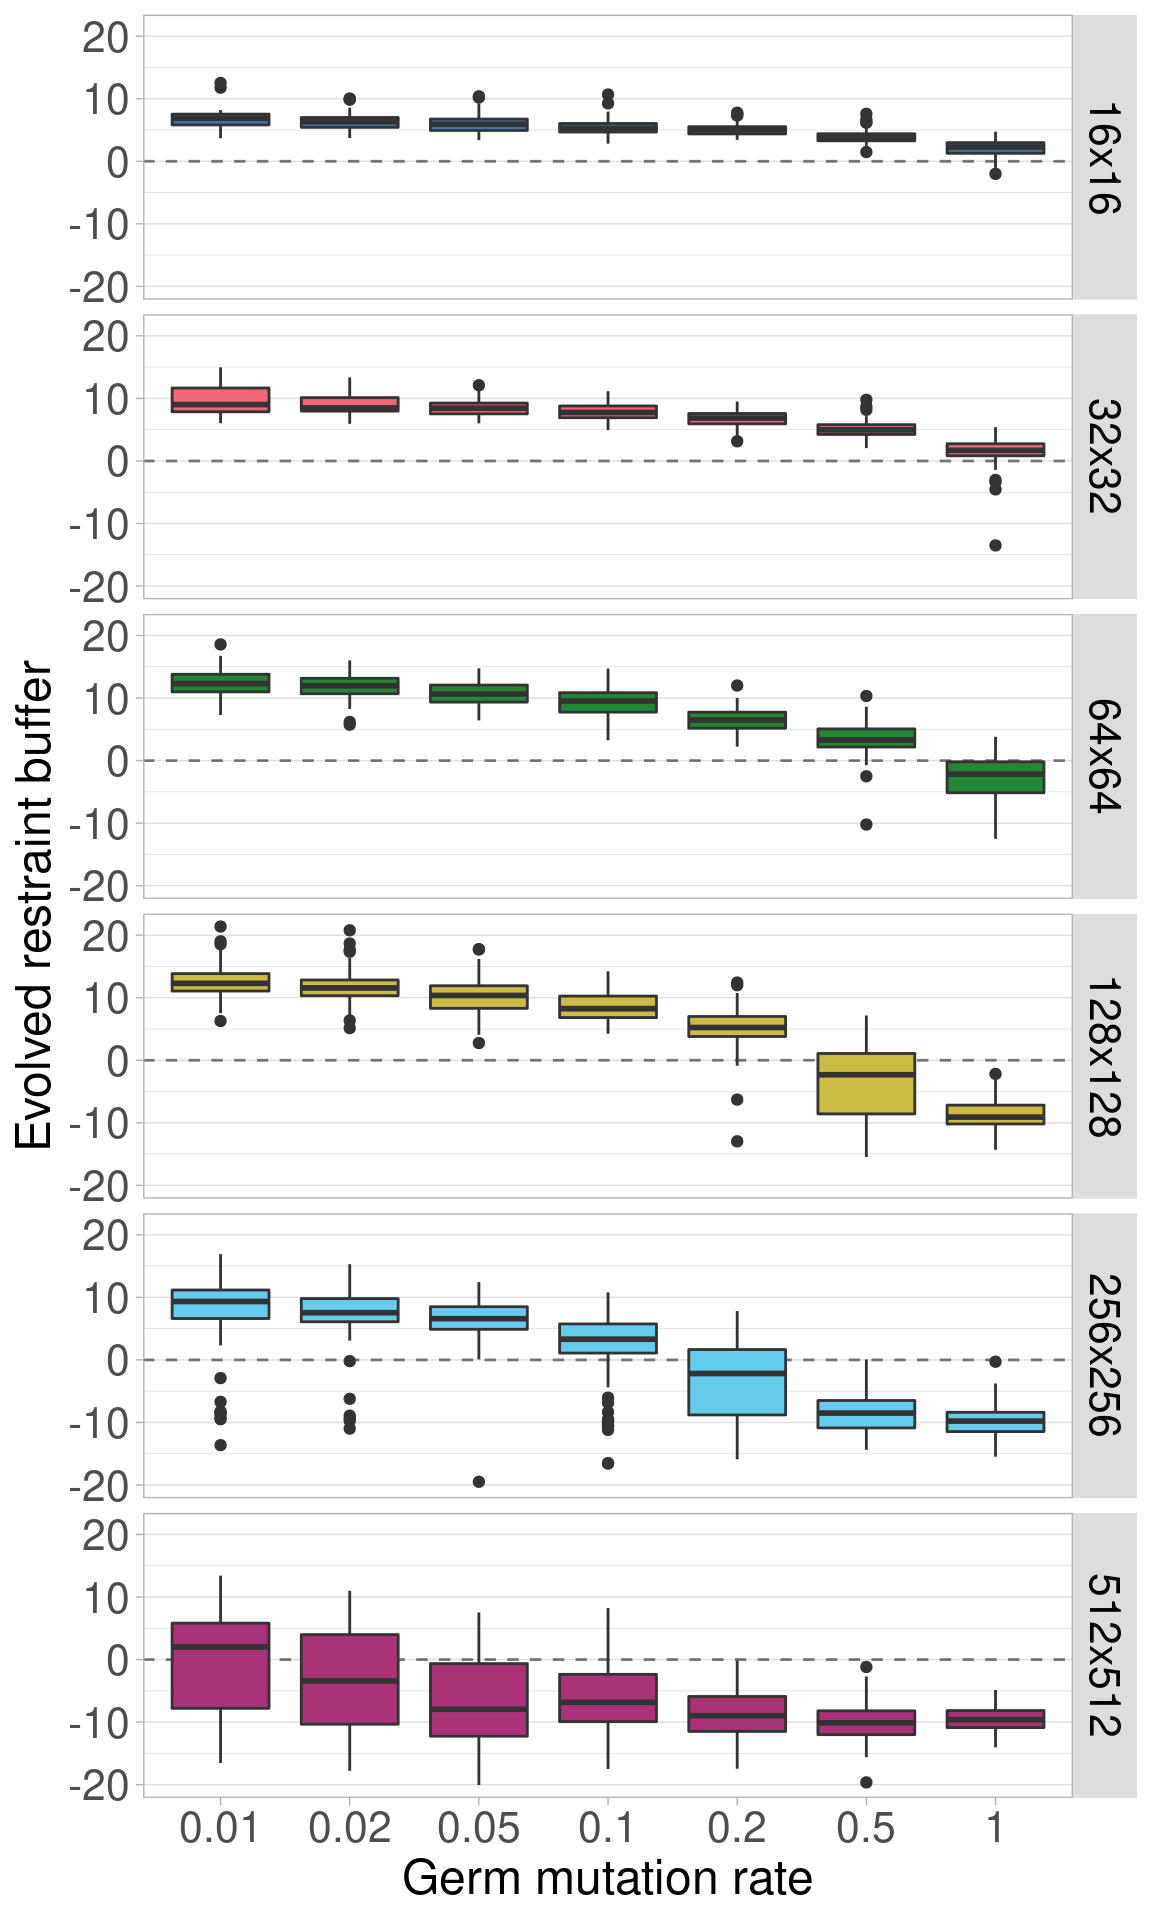
\includegraphics{primordium_supplemental_material_files/figure-latex/unnamed-chunk-41-1.pdf}

Again, we plot the same data again, but now the y-axis can change between rows.

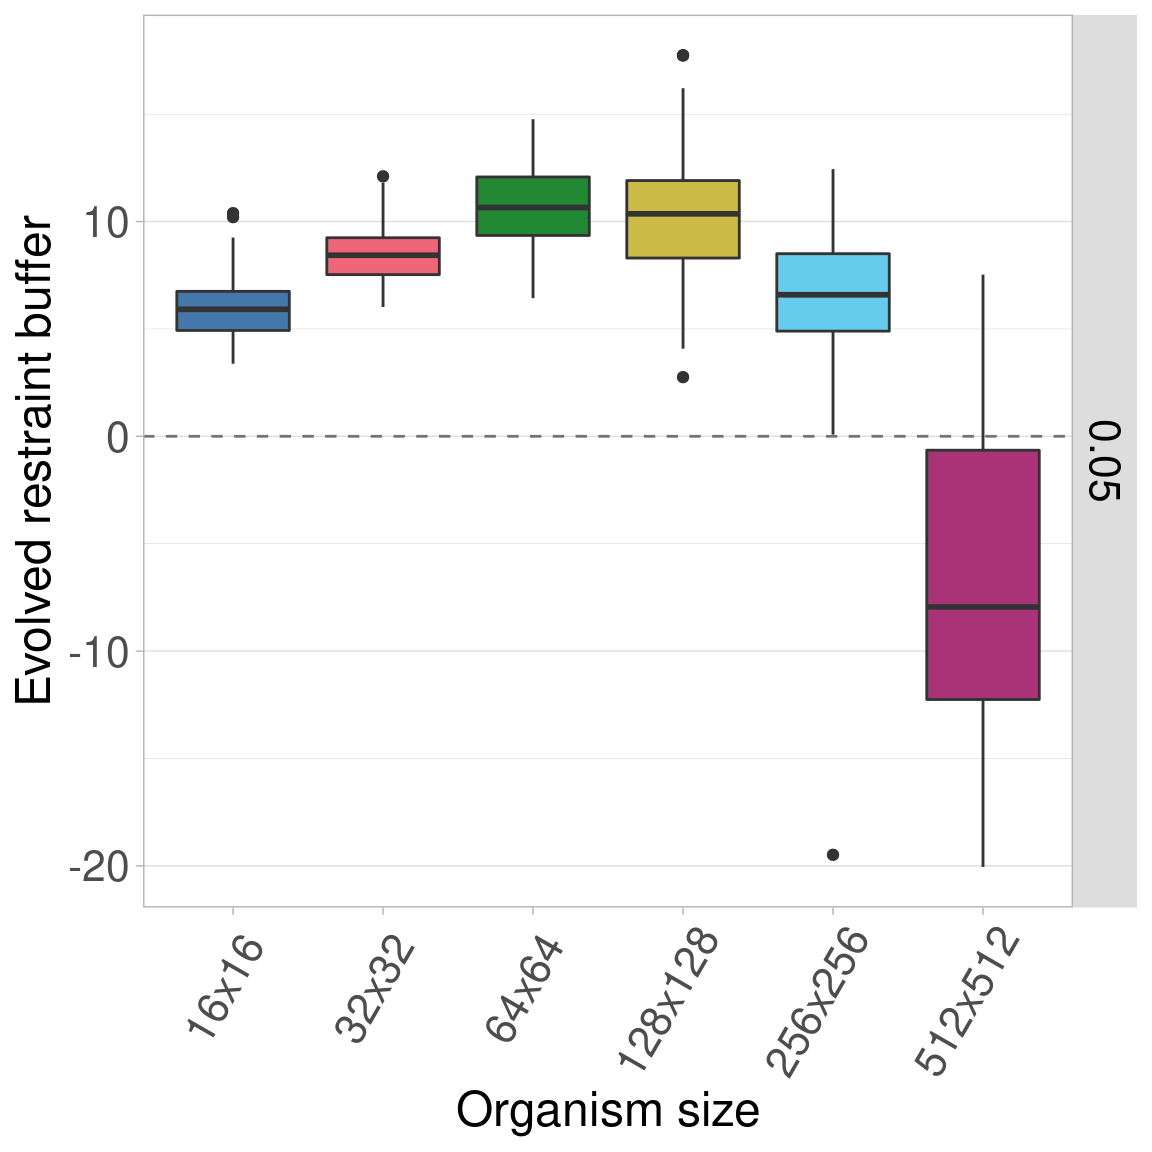
\includegraphics{primordium_supplemental_material_files/figure-latex/unnamed-chunk-42-1.pdf}

\hypertarget{single-organism-size-plots-1}{%
\section{Single organism size plots}\label{single-organism-size-plots-1}}

Here we plot each organism size independently, with the germ mutation rate on the x-axis.

\hypertarget{organism-size-16x16-1}{%
\subsection{Organism size 16x16}\label{organism-size-16x16-1}}

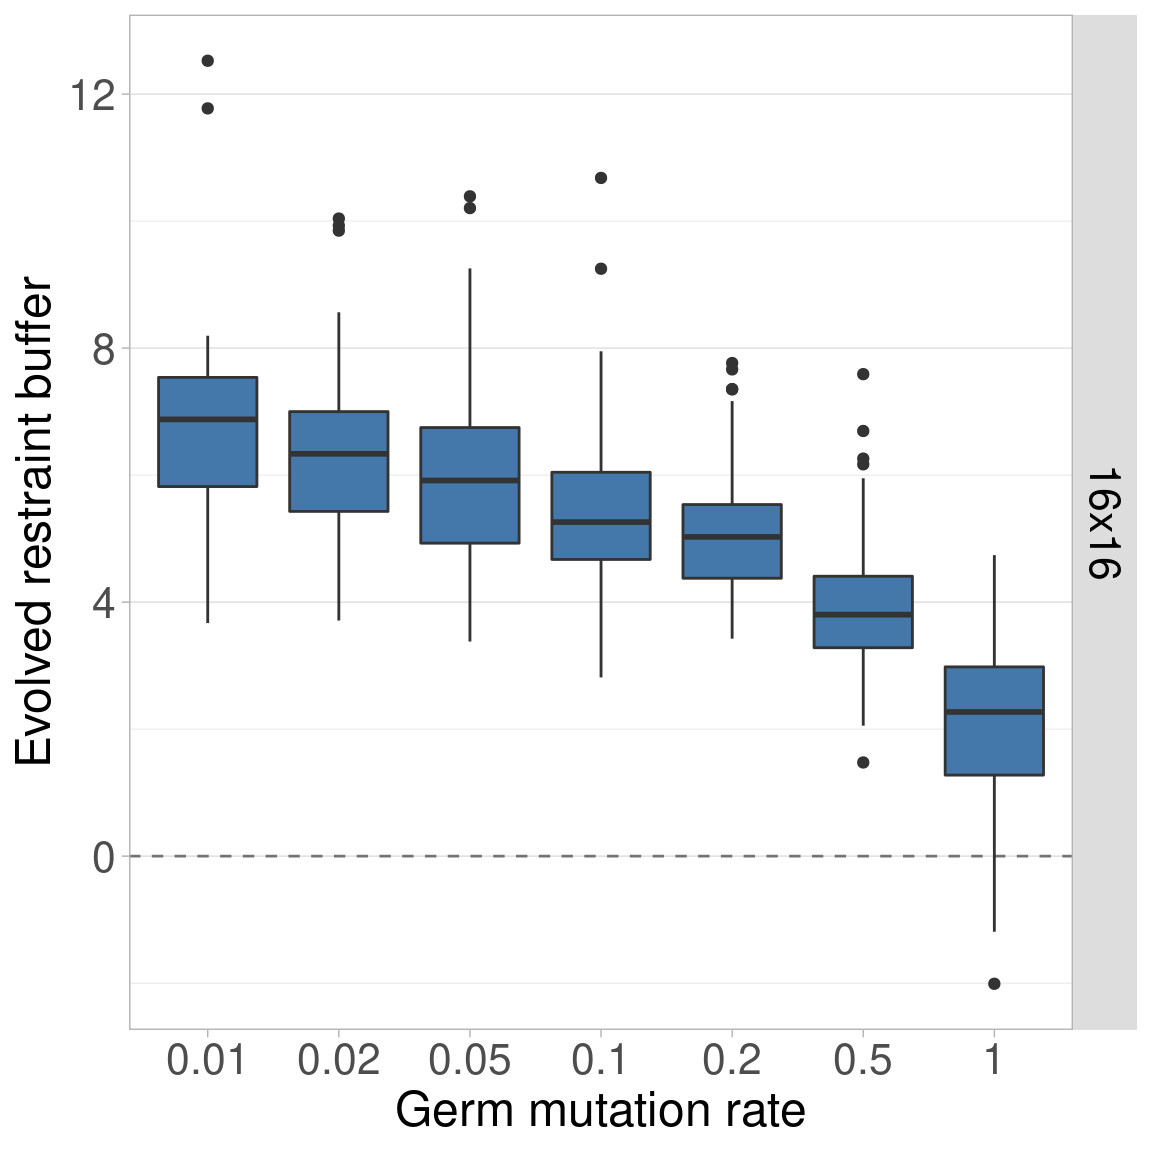
\includegraphics{primordium_supplemental_material_files/figure-latex/unnamed-chunk-43-1.pdf}

\hypertarget{organism-size-32x32-1}{%
\subsection{Organism size 32x32}\label{organism-size-32x32-1}}

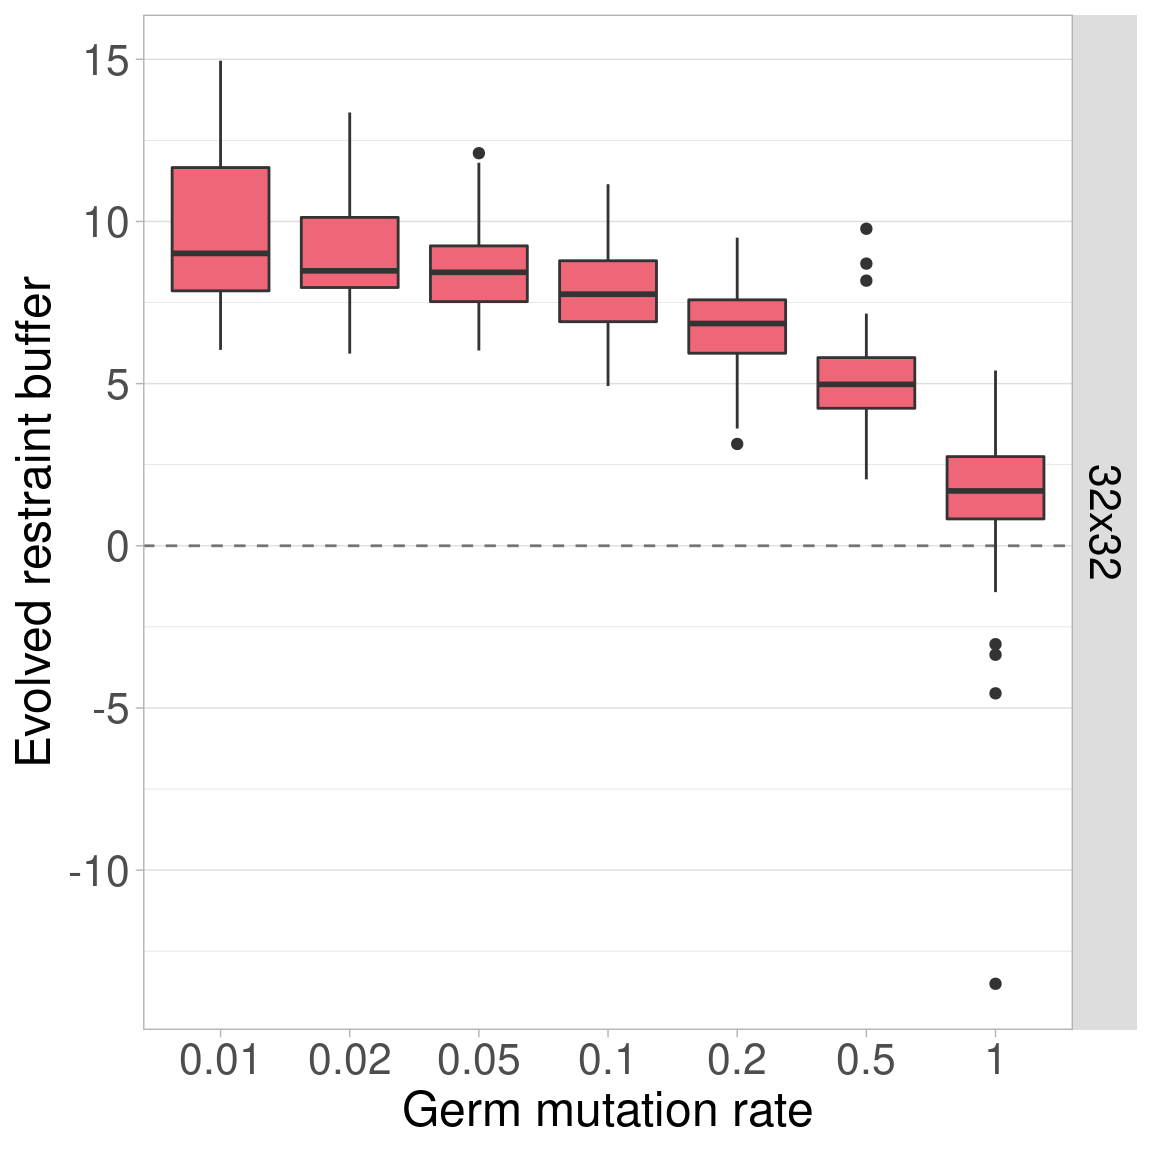
\includegraphics{primordium_supplemental_material_files/figure-latex/unnamed-chunk-44-1.pdf}

\hypertarget{organism-size-64x64-1}{%
\subsection{Organism size 64x64}\label{organism-size-64x64-1}}

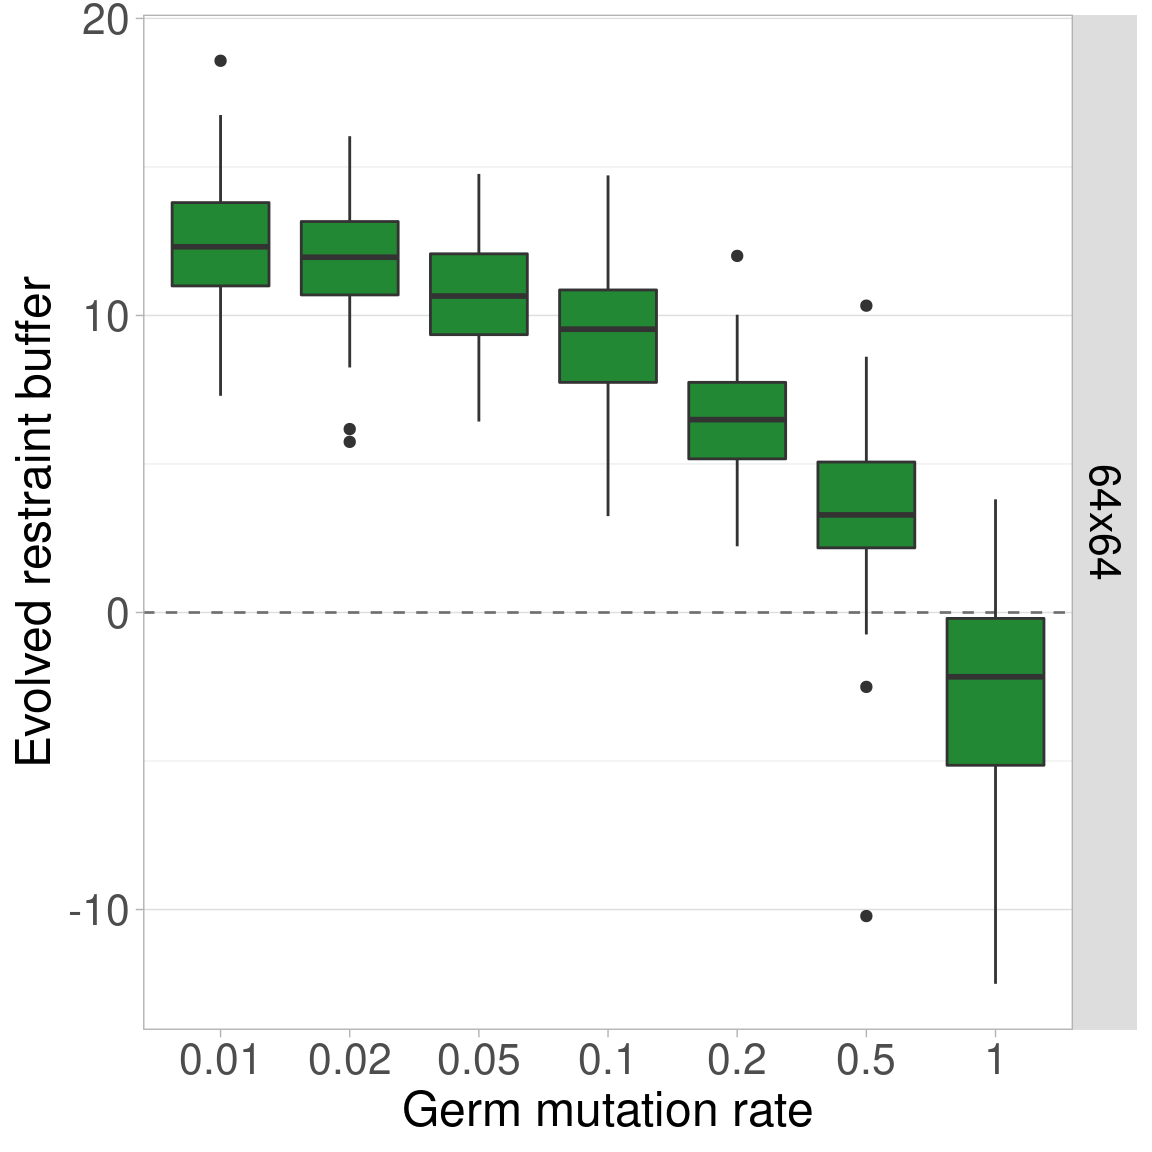
\includegraphics{primordium_supplemental_material_files/figure-latex/unnamed-chunk-45-1.pdf}

\hypertarget{organism-size-128x128-1}{%
\subsection{Organism size 128x128}\label{organism-size-128x128-1}}

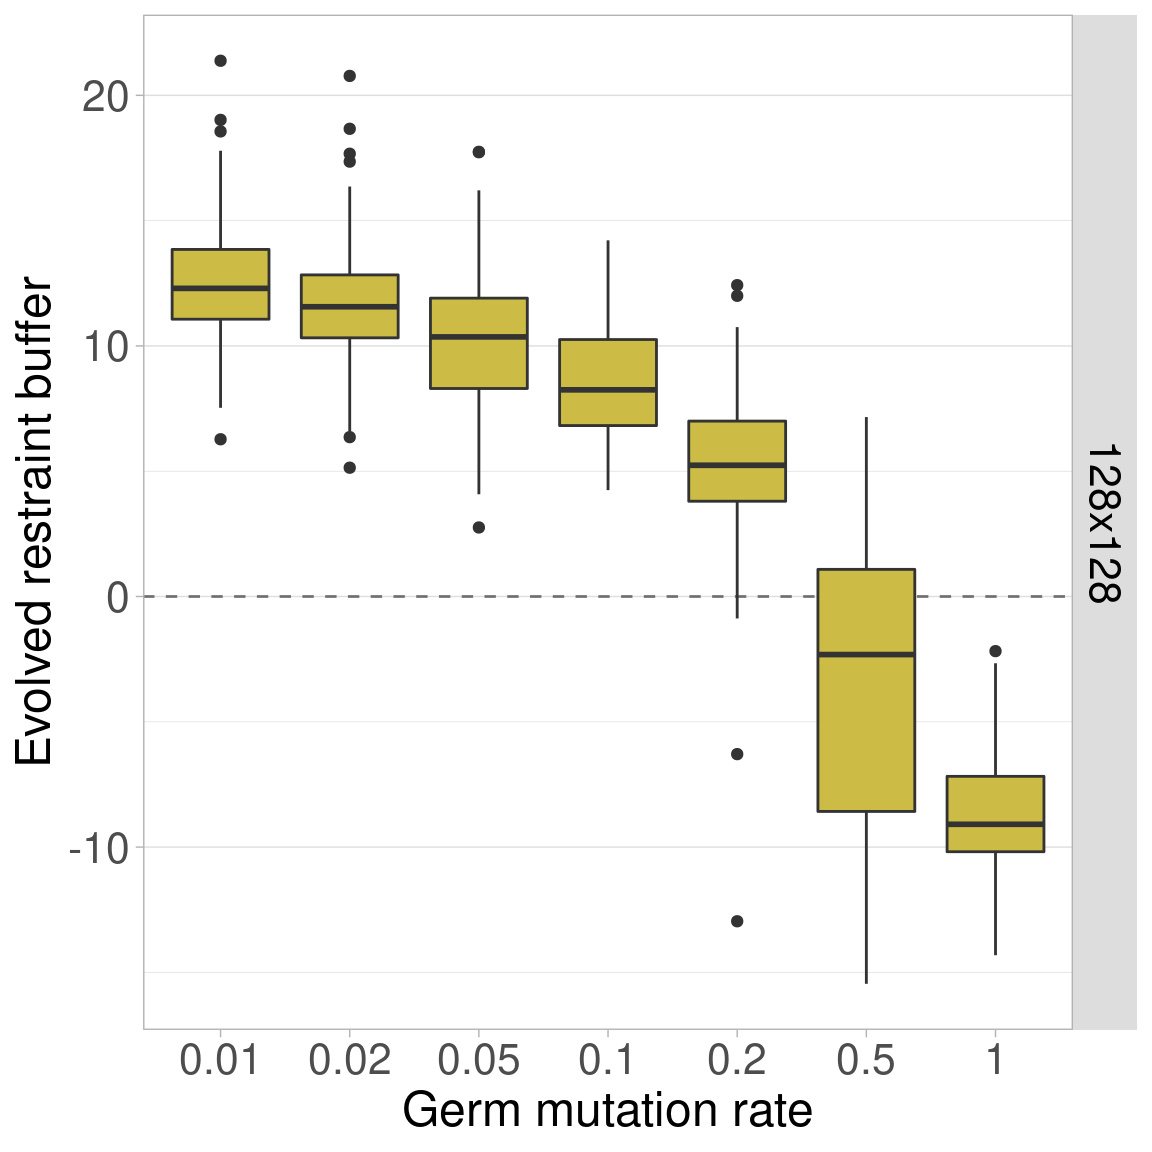
\includegraphics{primordium_supplemental_material_files/figure-latex/unnamed-chunk-46-1.pdf}

\hypertarget{organism-size-256x256-1}{%
\subsection{Organism size 256x256}\label{organism-size-256x256-1}}

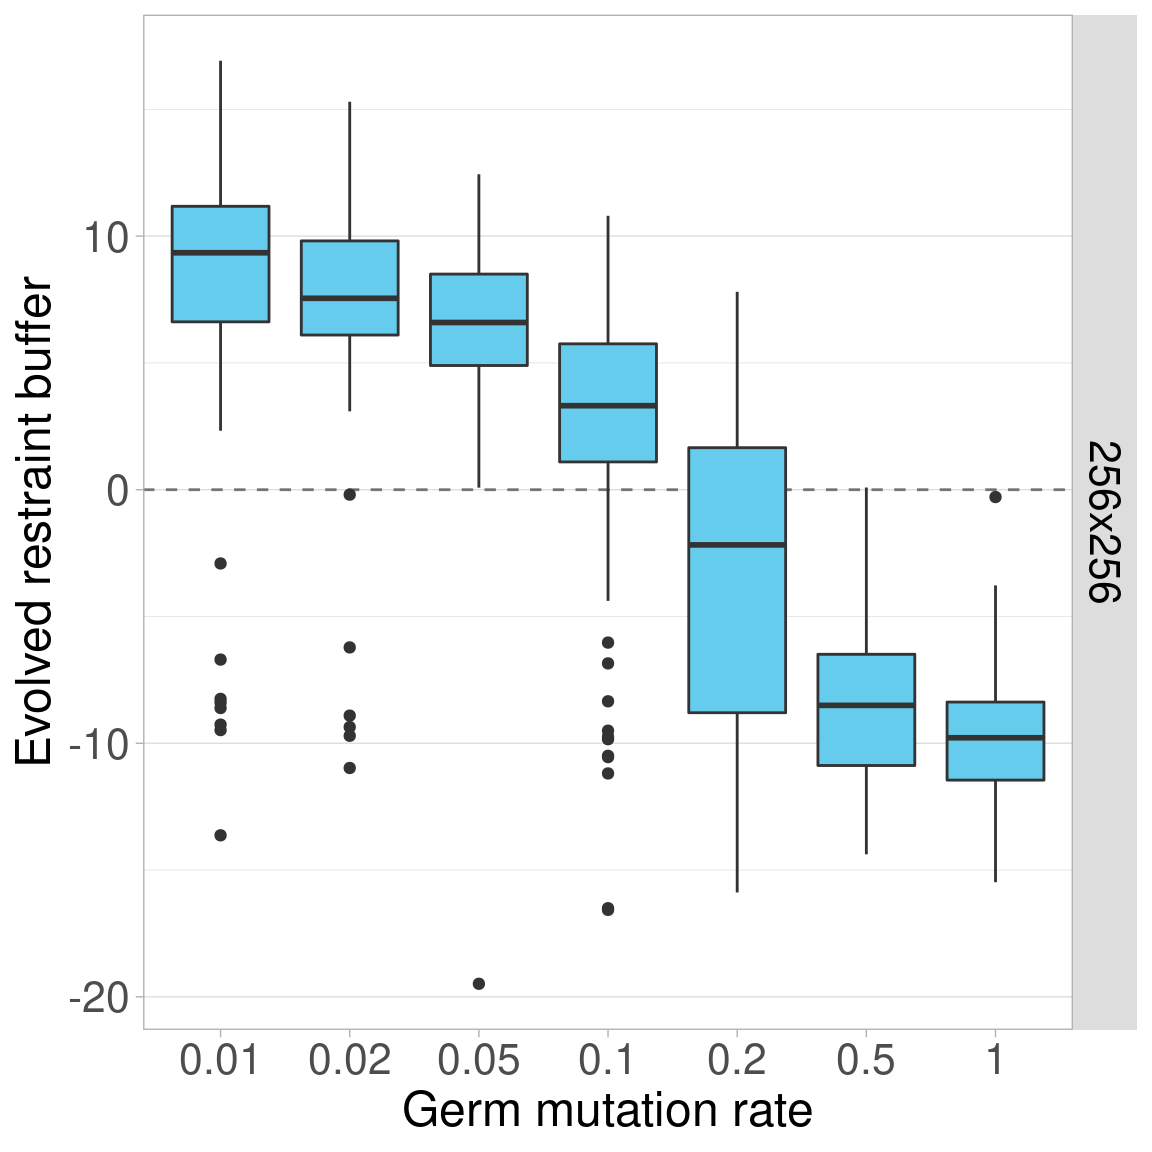
\includegraphics{primordium_supplemental_material_files/figure-latex/unnamed-chunk-47-1.pdf}

\hypertarget{organism-size-512x512-1}{%
\subsection{Organism size 512x512}\label{organism-size-512x512-1}}

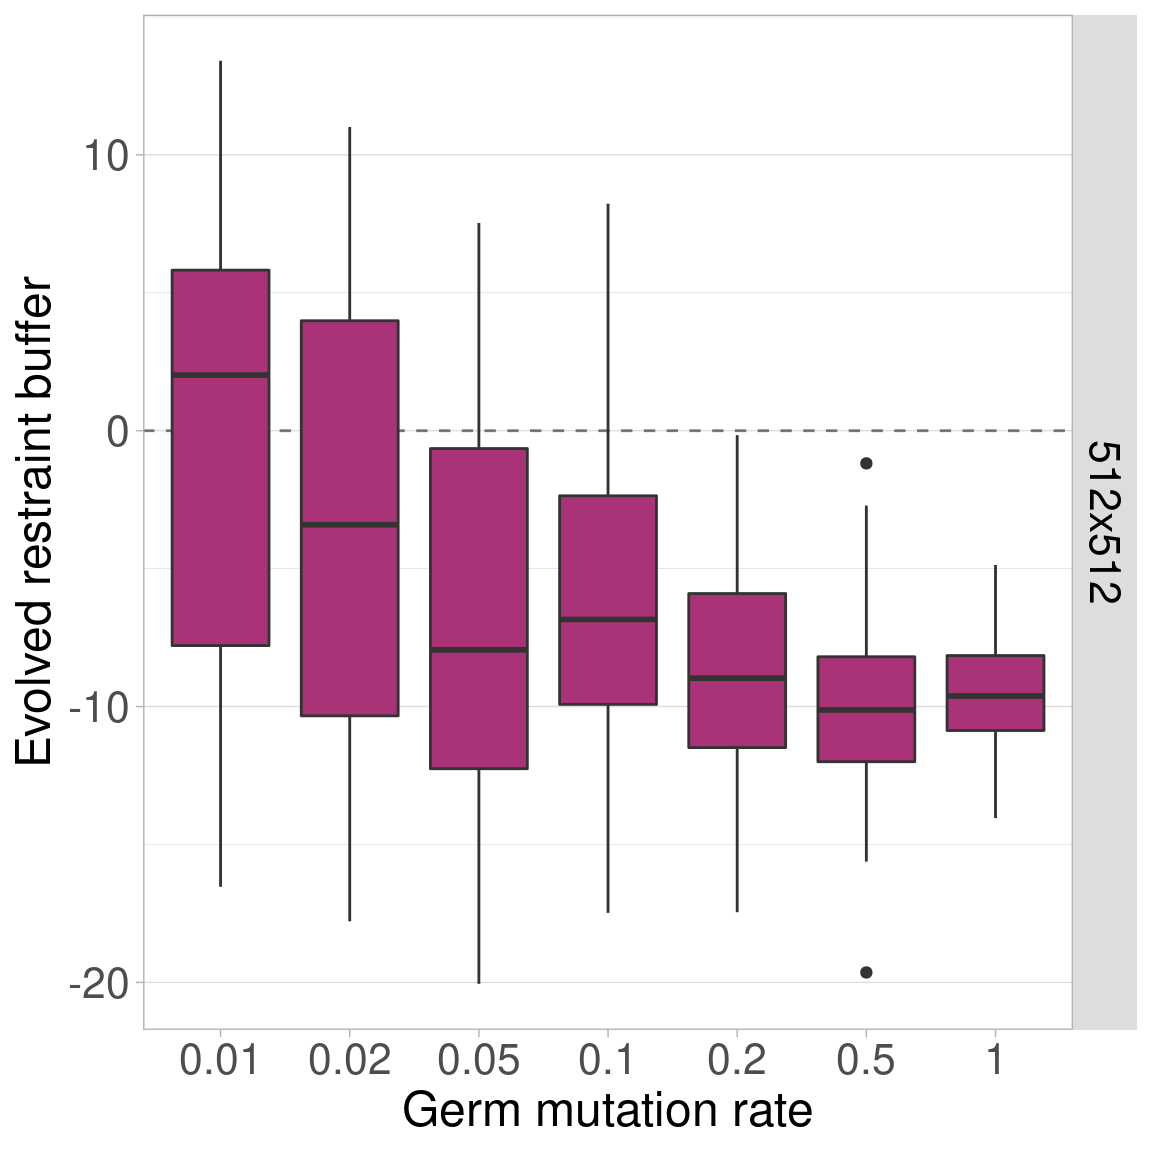
\includegraphics{primordium_supplemental_material_files/figure-latex/unnamed-chunk-48-1.pdf}

\hypertarget{single-organism-size-plots-2}{%
\section{Single organism size plots}\label{single-organism-size-plots-2}}

Similarly, here we plot each germ mutation rate independently, with the organism size on the x-axis.

\hypertarget{germ-mut.-rate-0.01}{%
\subsection{Germ mut. rate 0.01}\label{germ-mut.-rate-0.01}}

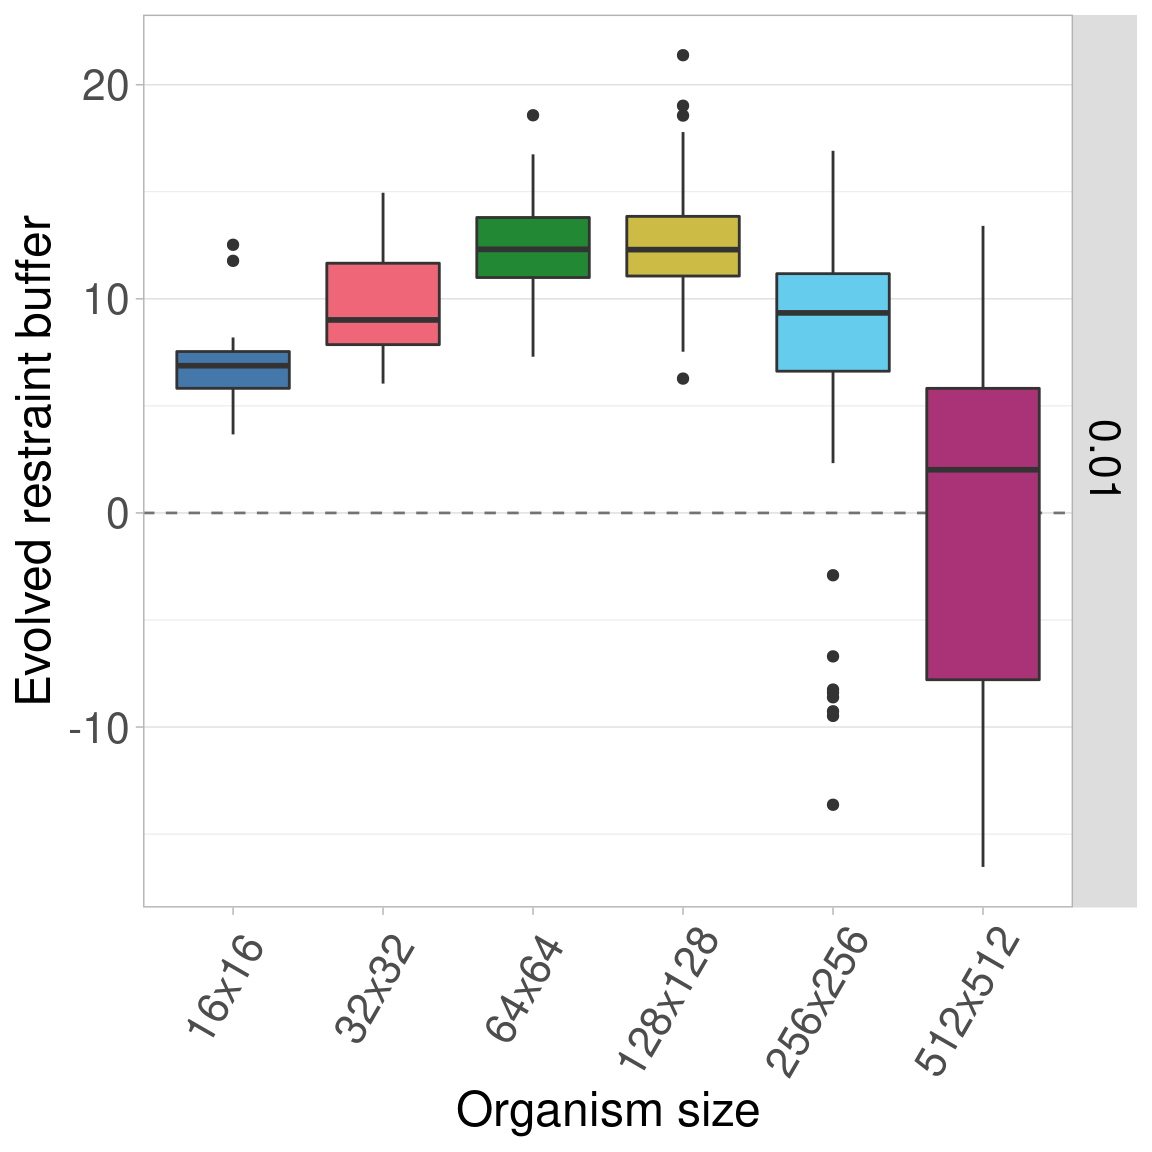
\includegraphics{primordium_supplemental_material_files/figure-latex/unnamed-chunk-49-1.pdf}

\hypertarget{germ-mut.-rate-0.02}{%
\subsection{Germ mut. rate 0.02}\label{germ-mut.-rate-0.02}}

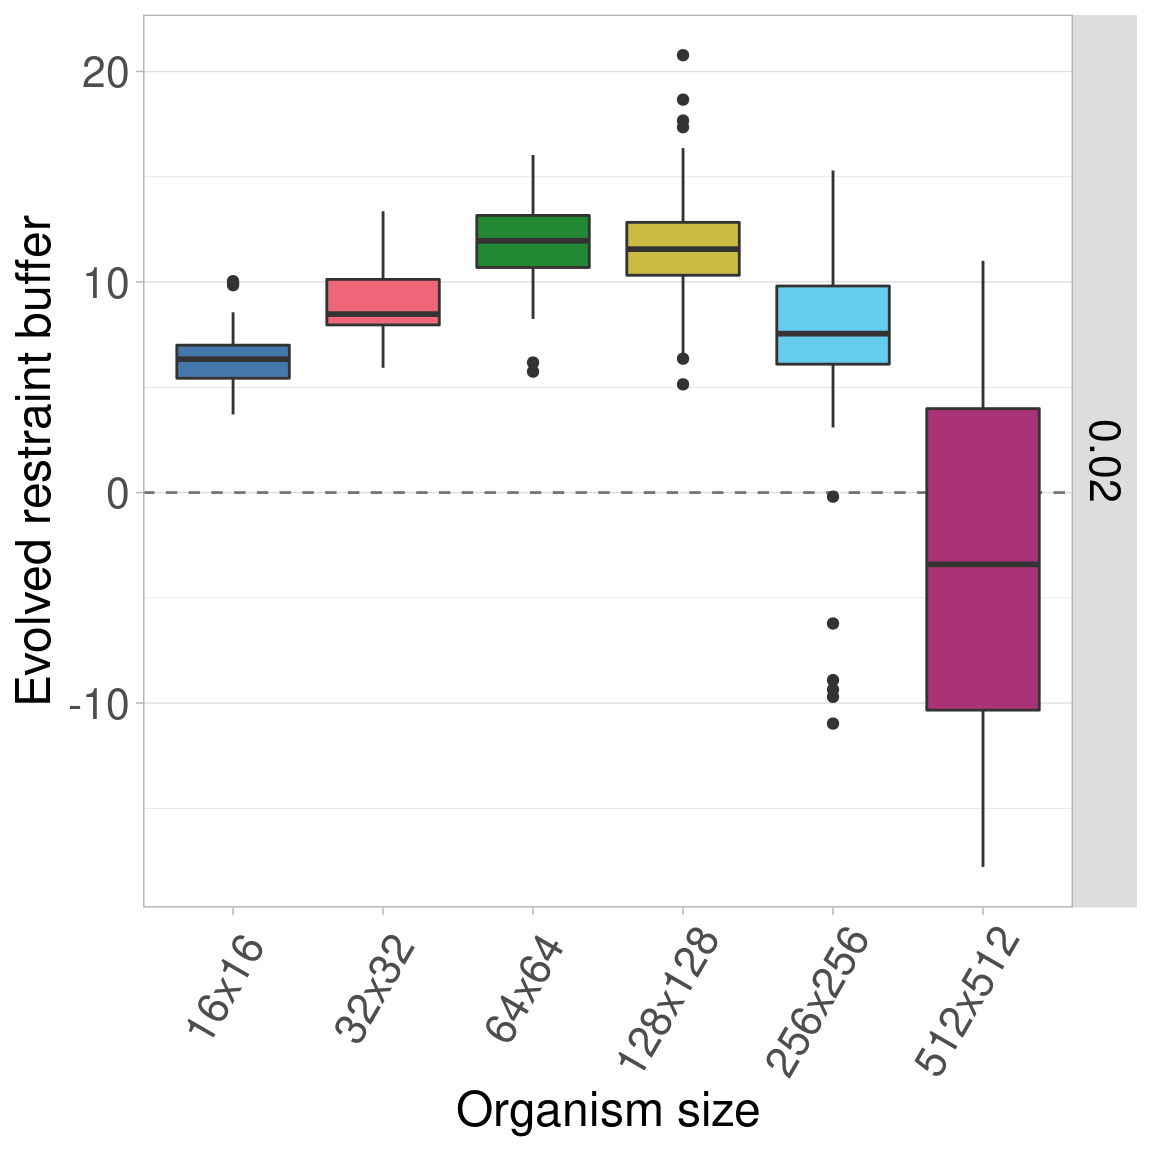
\includegraphics{primordium_supplemental_material_files/figure-latex/unnamed-chunk-50-1.pdf}

\hypertarget{germ-mut.-rate-0.05}{%
\subsection{Germ mut. rate 0.05}\label{germ-mut.-rate-0.05}}

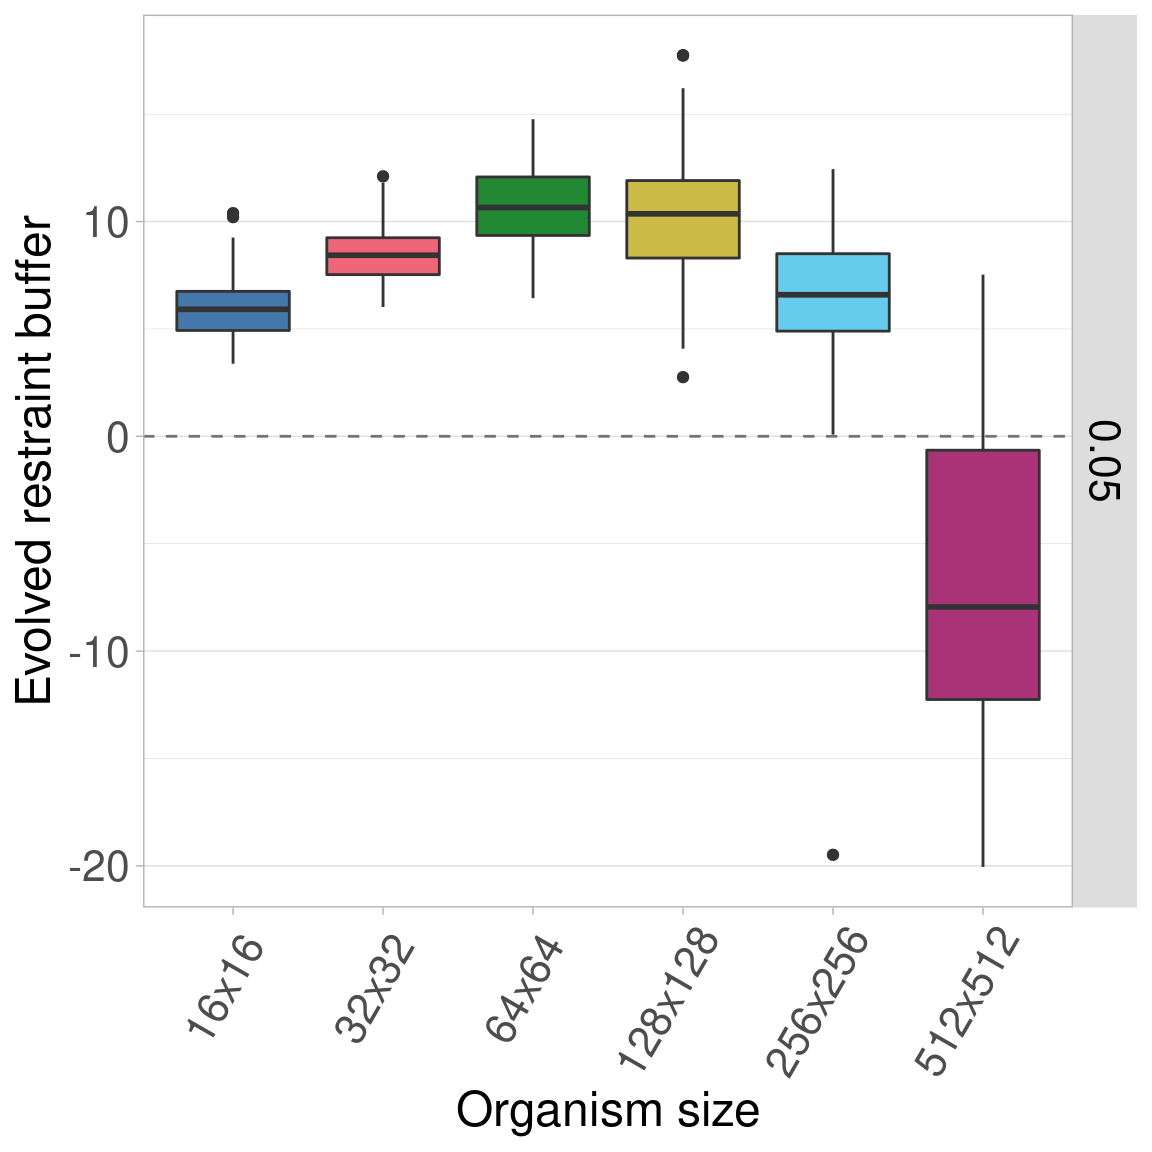
\includegraphics{primordium_supplemental_material_files/figure-latex/unnamed-chunk-51-1.pdf}

\hypertarget{germ-mut.-rate-0.1}{%
\subsection{Germ mut. rate 0.1}\label{germ-mut.-rate-0.1}}

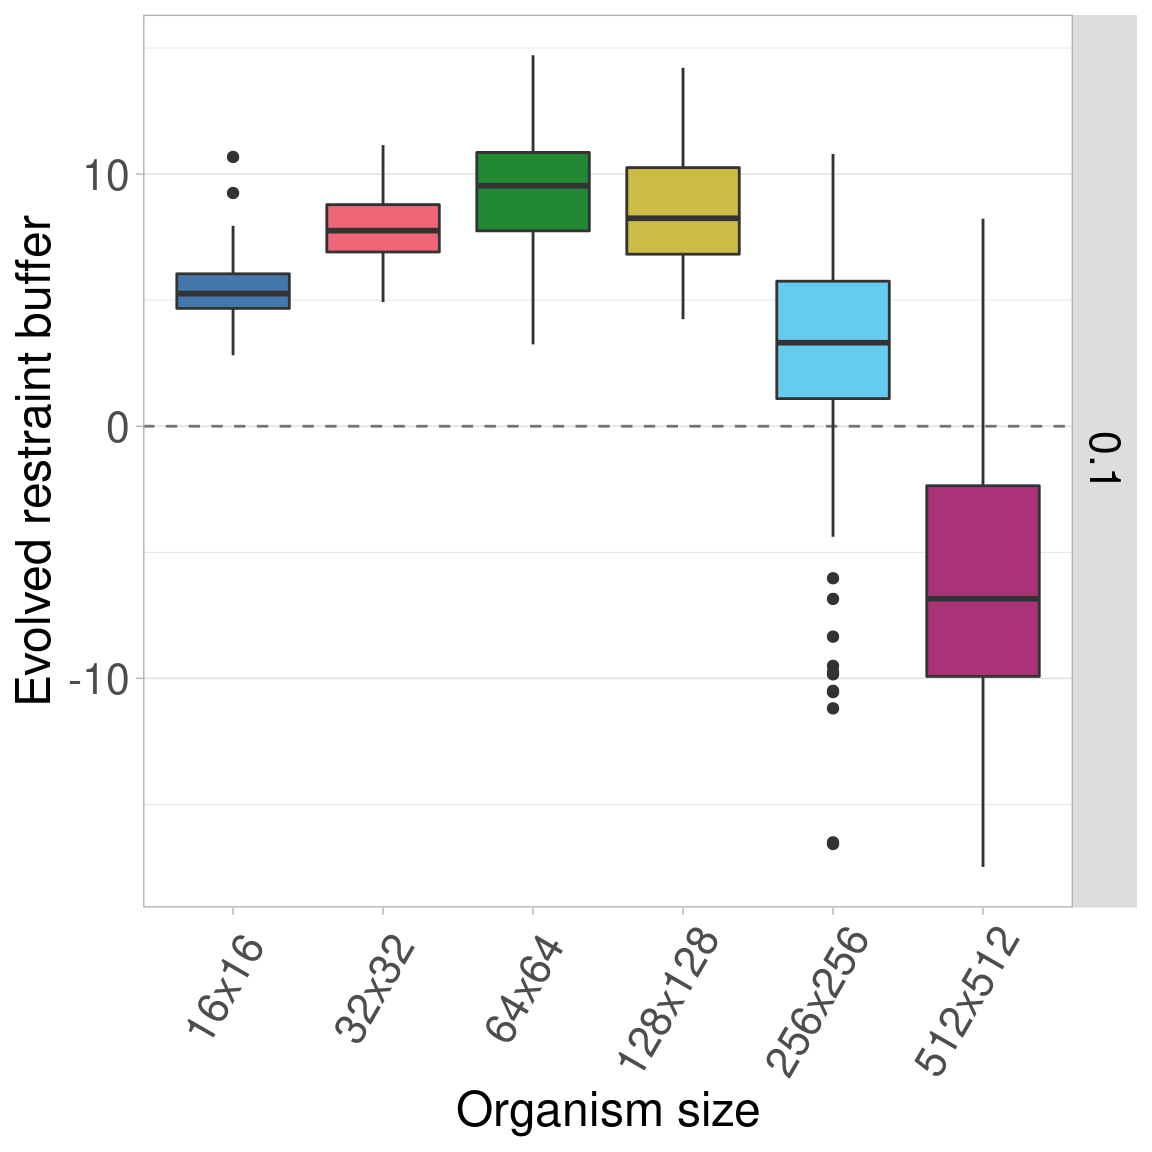
\includegraphics{primordium_supplemental_material_files/figure-latex/unnamed-chunk-52-1.pdf}

\hypertarget{germ-mut.-rate-0.2}{%
\subsection{Germ mut. rate 0.2}\label{germ-mut.-rate-0.2}}

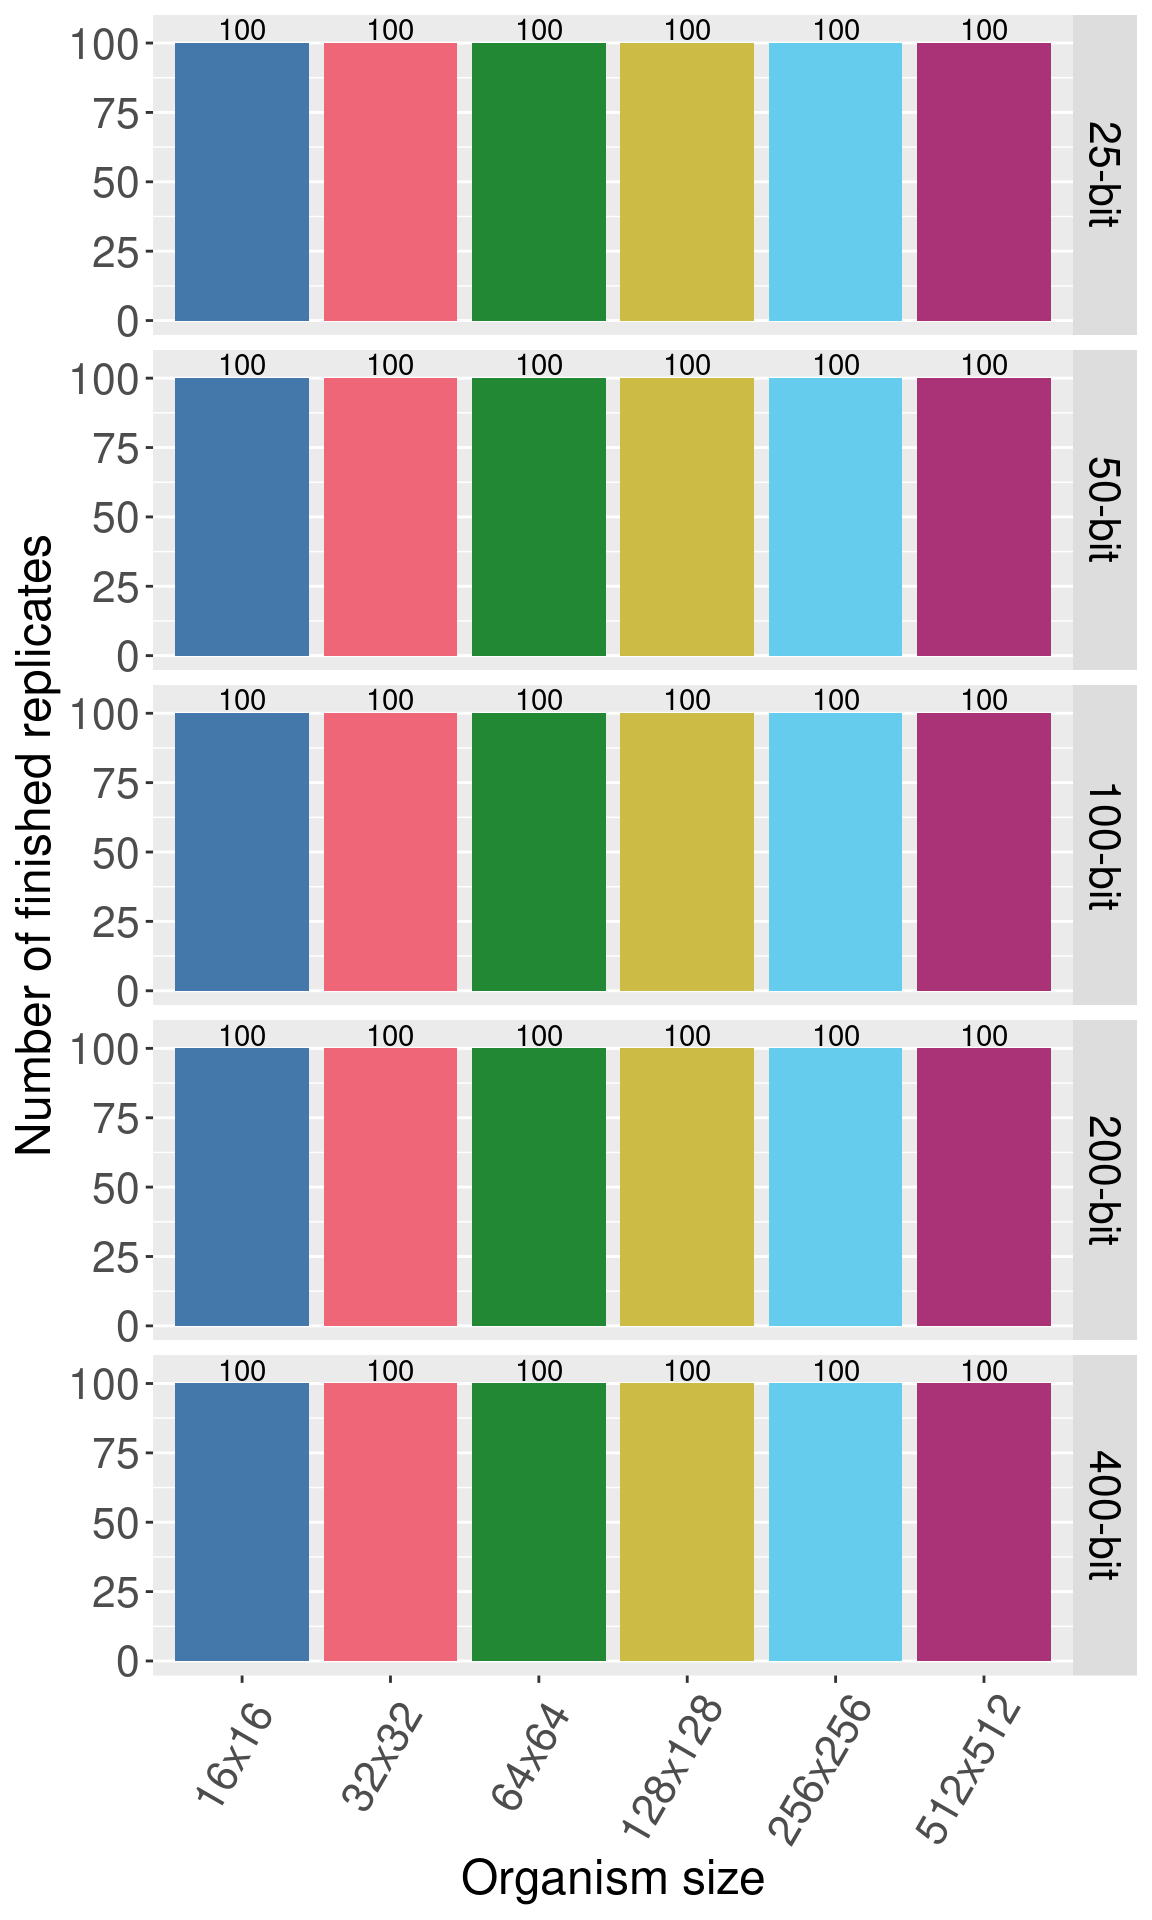
\includegraphics{primordium_supplemental_material_files/figure-latex/unnamed-chunk-53-1.pdf}

\hypertarget{germ-mut.-rate-0.5}{%
\subsection{Germ mut. rate 0.5}\label{germ-mut.-rate-0.5}}

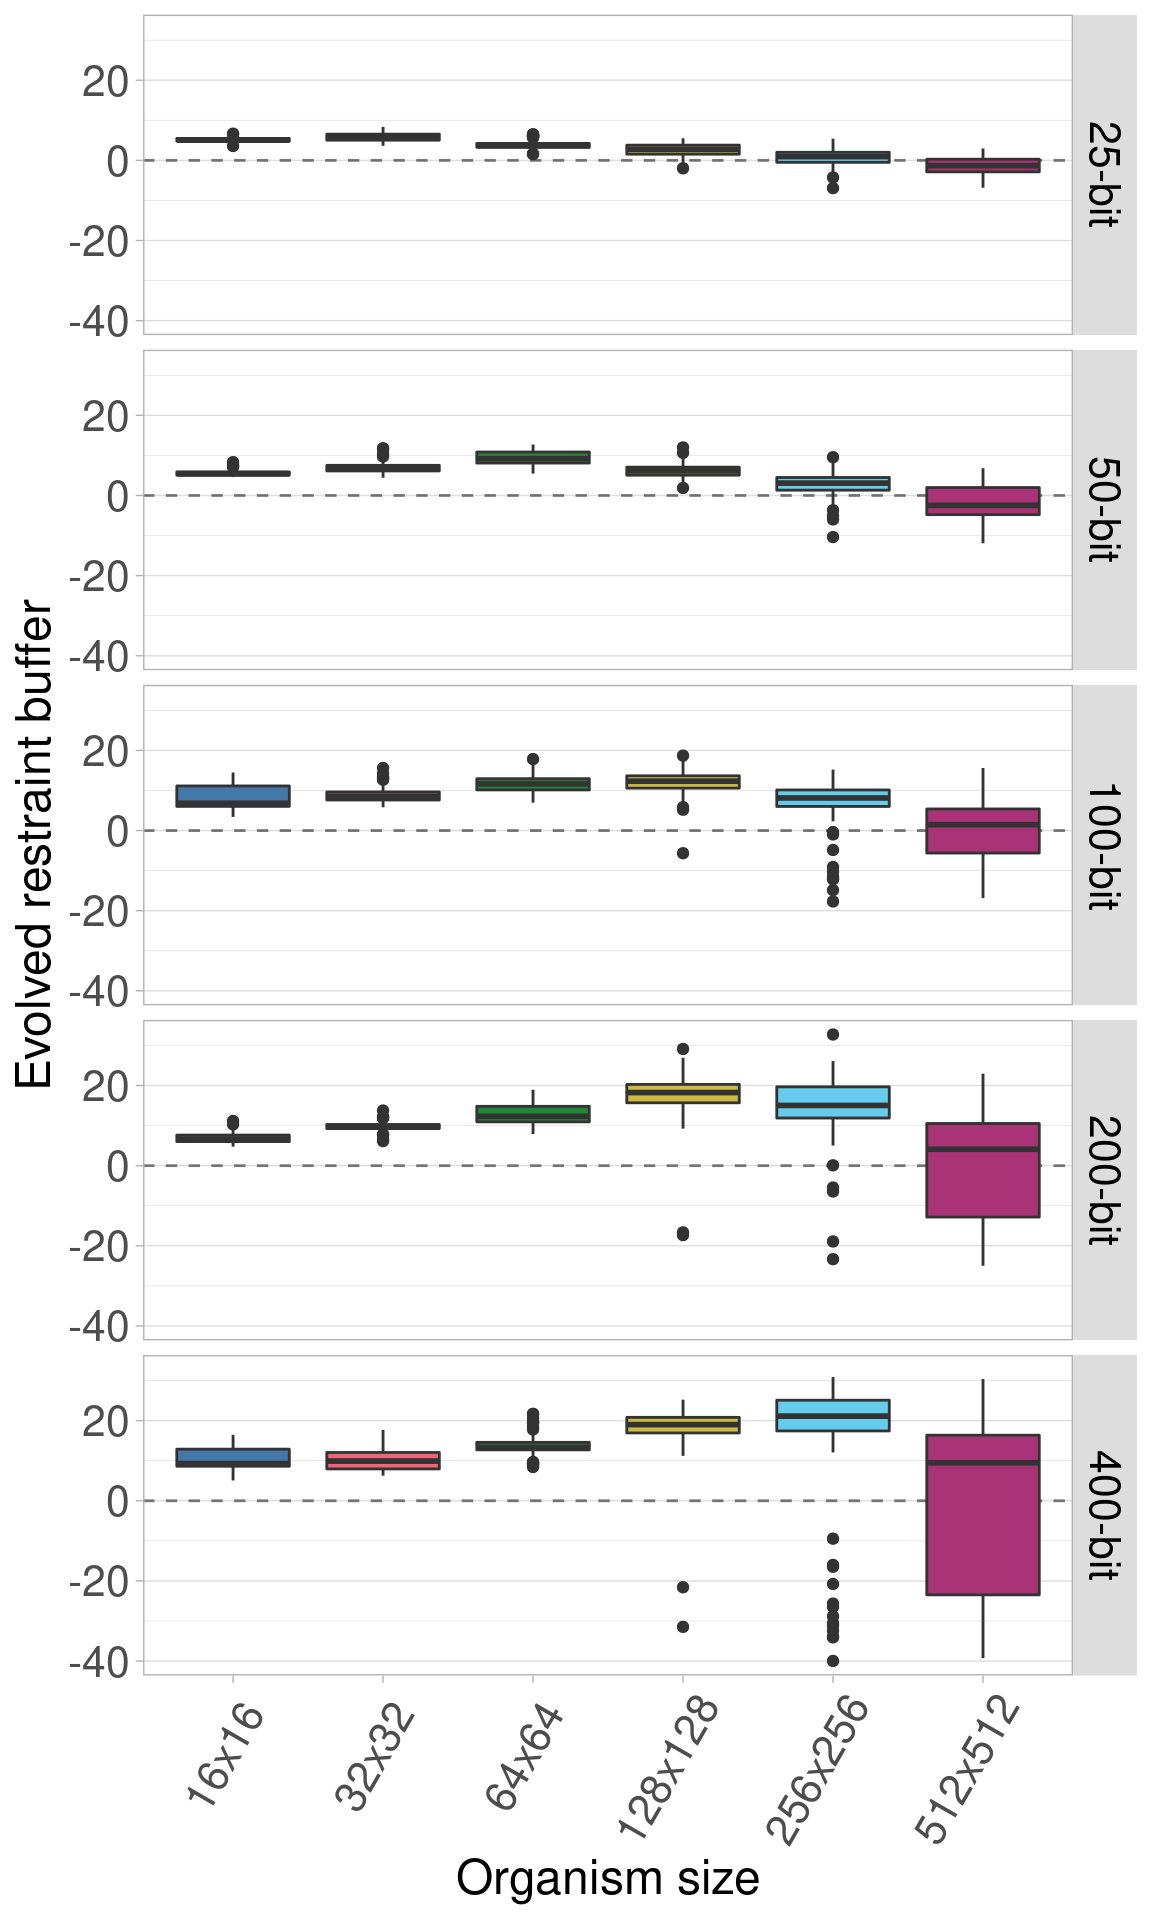
\includegraphics{primordium_supplemental_material_files/figure-latex/unnamed-chunk-54-1.pdf}

\hypertarget{germ-mut.-rate-1.0}{%
\subsection{Germ mut. rate 1.0}\label{germ-mut.-rate-1.0}}

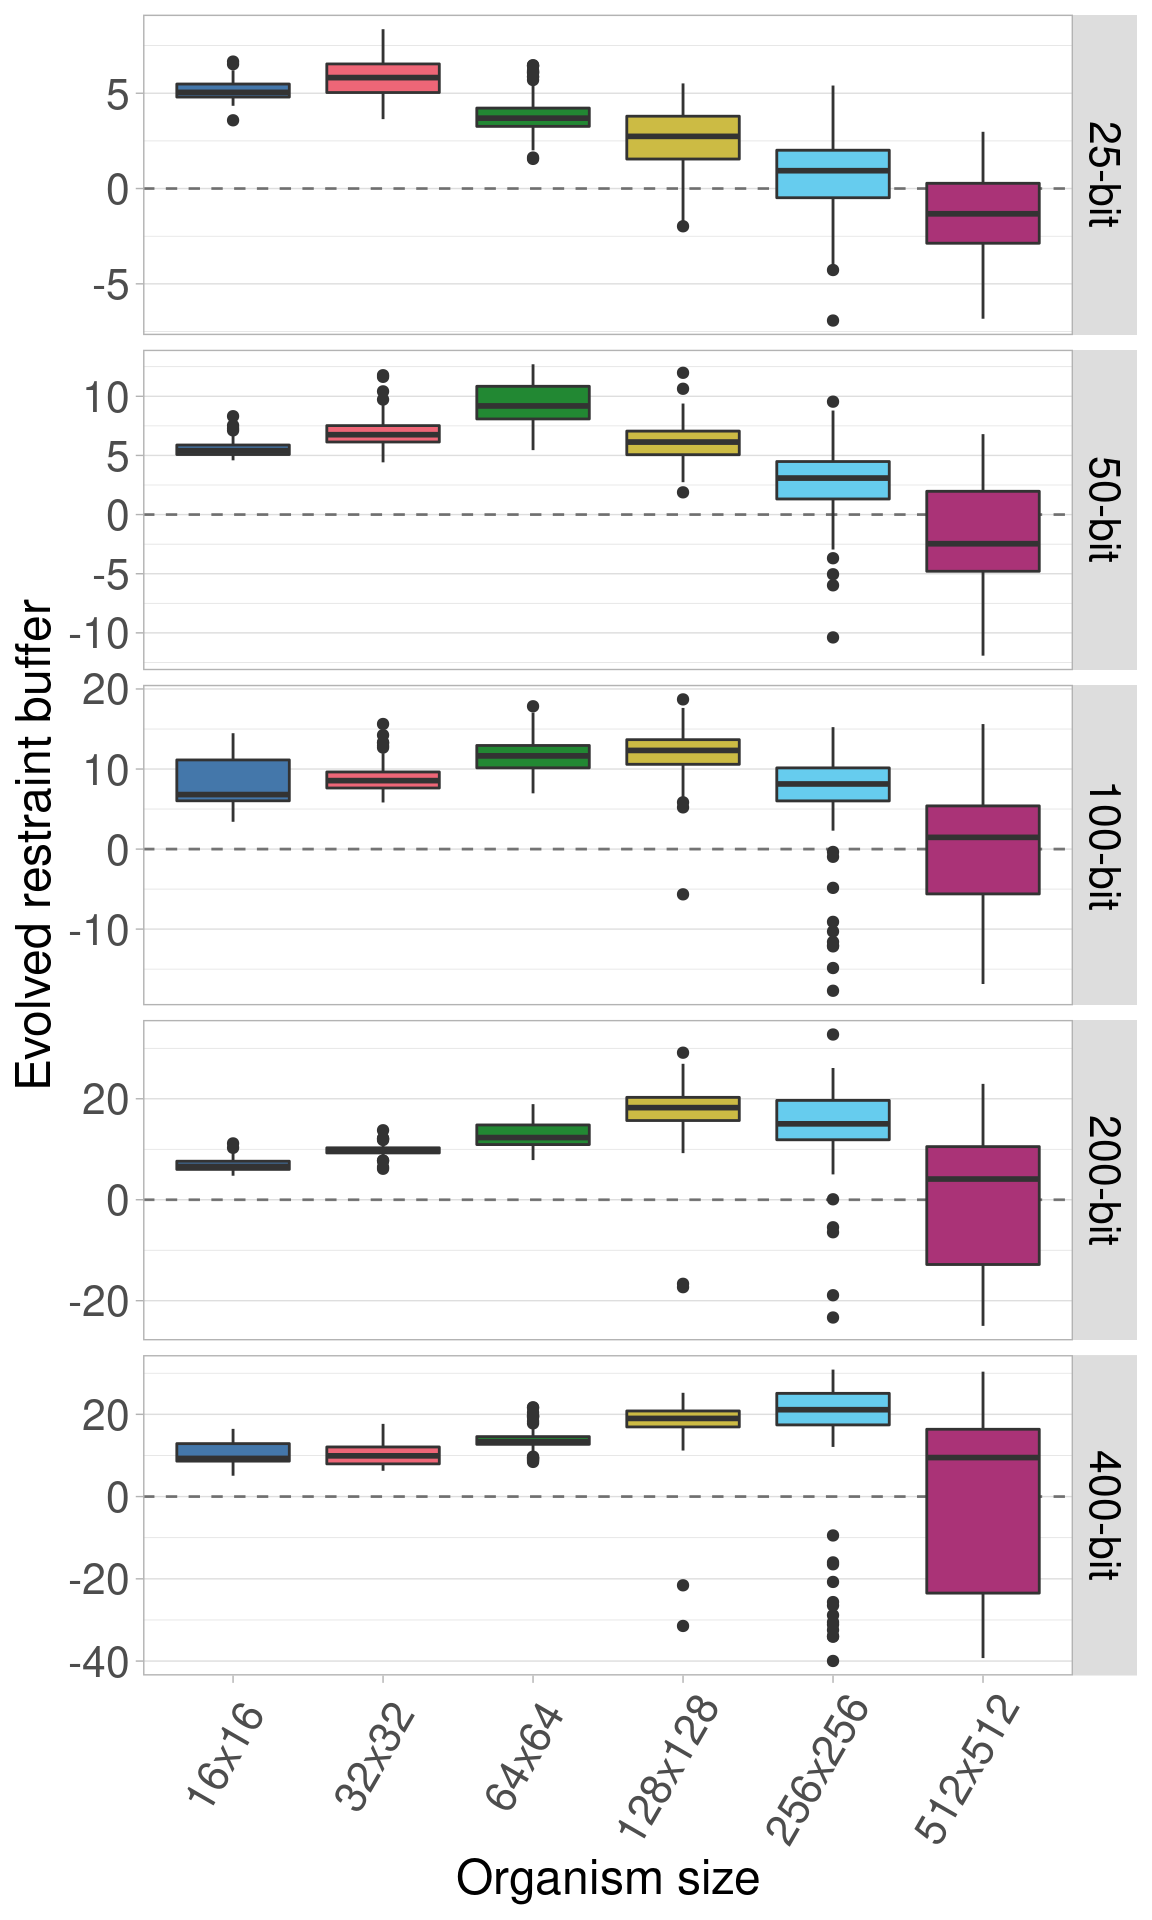
\includegraphics{primordium_supplemental_material_files/figure-latex/unnamed-chunk-55-1.pdf}

\hypertarget{statistics-2}{%
\section{Statistics}\label{statistics-2}}

Since organism size is our main point of comparison, we calculate stats for each germ mutation rate.

First, we perform a Kruskal-Wallis test across all organism sizes to indicate if variance exists at that mutation rate.
If variance exists, we then perfrm a pairwise Wilcoxon Rank-Sum test to show which pairs of organism sizes significantly differ.
Finally, we perform Bonferroni-Holm corrections for multiple comparisons.

\begin{Shaded}
\begin{Highlighting}[]
\NormalTok{  mut_vec =}\StringTok{ }\KeywordTok{c}\NormalTok{(}\FloatTok{0.01}\NormalTok{, }\FloatTok{0.02}\NormalTok{, }\FloatTok{0.05}\NormalTok{, }\FloatTok{0.1}\NormalTok{, }\FloatTok{0.2}\NormalTok{, }\FloatTok{0.5}\NormalTok{, }\DecValTok{1}\NormalTok{)}
\NormalTok{  df_kruskal =}\StringTok{ }\KeywordTok{data.frame}\NormalTok{(}\DataTypeTok{data =} \KeywordTok{matrix}\NormalTok{(}\DataTypeTok{nrow =} \DecValTok{0}\NormalTok{, }\DataTypeTok{ncol =} \DecValTok{4}\NormalTok{))}
  \KeywordTok{colnames}\NormalTok{(df_kruskal) =}\StringTok{ }\KeywordTok{c}\NormalTok{(}\StringTok{'germ_mut_rate'}\NormalTok{, }\StringTok{'p_value'}\NormalTok{, }\StringTok{'chi_squared'}\NormalTok{, }\StringTok{'df'}\NormalTok{)}
  \ControlFlowTok{for}\NormalTok{(mut_rate }\ControlFlowTok{in}\NormalTok{ mut_vec)\{}
\NormalTok{    df_test =}\StringTok{ }\NormalTok{df2[df2}\OperatorTok{$}\NormalTok{MUT }\OperatorTok{==}\StringTok{ }\NormalTok{mut_rate,]}
\NormalTok{    res =}\StringTok{ }\KeywordTok{kruskal.test}\NormalTok{(df_test}\OperatorTok{$}\NormalTok{restraint_value }\OperatorTok{~}\StringTok{ }\NormalTok{df_test}\OperatorTok{$}\NormalTok{MCSIZE, df_test)}
\NormalTok{    df_kruskal[}\KeywordTok{nrow}\NormalTok{(df_kruskal) }\OperatorTok{+}\StringTok{ }\DecValTok{1}\NormalTok{,] =}\StringTok{ }\KeywordTok{c}\NormalTok{(mut_rate, res}\OperatorTok{$}\NormalTok{p.value, }\KeywordTok{as.numeric}\NormalTok{(res}\OperatorTok{$}\NormalTok{statistic)[}\DecValTok{1}\NormalTok{], }\KeywordTok{as.numeric}\NormalTok{(res}\OperatorTok{$}\NormalTok{parameter)[}\DecValTok{1}\NormalTok{])}
\NormalTok{  \}}
\NormalTok{  df_kruskal}\OperatorTok{$}\NormalTok{less_}\FloatTok{0.01}\NormalTok{ =}\StringTok{ }\NormalTok{df_kruskal}\OperatorTok{$}\NormalTok{p_value }\OperatorTok{<}\StringTok{ }\FloatTok{0.01}
  \KeywordTok{print}\NormalTok{(df_kruskal)}
\end{Highlighting}
\end{Shaded}

\begin{verbatim}
##   germ_mut_rate      p_value chi_squared df less_0.01
## 1          0.01 9.191452e-79    374.5160  5      TRUE
## 2          0.02 6.227269e-82    389.2251  5      TRUE
## 3          0.05 1.934895e-82    391.5809  5      TRUE
## 4          0.10 1.983976e-83    396.1708  5      TRUE
## 5          0.20 3.180895e-85    404.4991  5      TRUE
## 6          0.50 4.313881e-91    431.7152  5      TRUE
## 7          1.00 2.144229e-92    437.7600  5      TRUE
\end{verbatim}

We see that significant variation exists within each mutation rate, so we perform pariwise Wilcoxon tests on each to see which pais of sizes are significantly different.

\begin{Shaded}
\begin{Highlighting}[]
\NormalTok{size_vec =}\StringTok{ }\KeywordTok{c}\NormalTok{(}\DecValTok{16}\NormalTok{, }\DecValTok{32}\NormalTok{, }\DecValTok{64}\NormalTok{, }\DecValTok{128}\NormalTok{, }\DecValTok{256}\NormalTok{, }\DecValTok{512}\NormalTok{)}
\NormalTok{mut_vec =}\StringTok{ }\KeywordTok{c}\NormalTok{(}\FloatTok{0.01}\NormalTok{, }\FloatTok{0.02}\NormalTok{, }\FloatTok{0.05}\NormalTok{, }\FloatTok{0.1}\NormalTok{, }\FloatTok{0.2}\NormalTok{, }\FloatTok{0.5}\NormalTok{, }\DecValTok{1}\NormalTok{)}
\ControlFlowTok{for}\NormalTok{(mut_rate }\ControlFlowTok{in}\NormalTok{ mut_vec)\{}
\NormalTok{  df_test =}\StringTok{ }\NormalTok{df2[df2}\OperatorTok{$}\NormalTok{MUT }\OperatorTok{==}\StringTok{ }\NormalTok{mut_rate,]}
\NormalTok{  df_wilcox =}\StringTok{ }\KeywordTok{data.frame}\NormalTok{(}\DataTypeTok{data =} \KeywordTok{matrix}\NormalTok{(}\DataTypeTok{nrow =} \DecValTok{0}\NormalTok{, }\DataTypeTok{ncol =} \DecValTok{6}\NormalTok{))}
  \KeywordTok{colnames}\NormalTok{(df_wilcox) =}\StringTok{ }\KeywordTok{c}\NormalTok{(}\StringTok{'germ_mut_rate'}\NormalTok{, }\StringTok{'size_a'}\NormalTok{, }\StringTok{'size_b'}\NormalTok{, }\StringTok{'p_value_corrected'}\NormalTok{, }\StringTok{'p_value_raw'}\NormalTok{, }\StringTok{'W'}\NormalTok{)}
  \ControlFlowTok{for}\NormalTok{(size_idx_a }\ControlFlowTok{in} \DecValTok{1}\OperatorTok{:}\NormalTok{(}\KeywordTok{length}\NormalTok{(size_vec) }\OperatorTok{-}\StringTok{ }\DecValTok{1}\NormalTok{))\{}
\NormalTok{    size_a =}\StringTok{ }\NormalTok{size_vec[size_idx_a]}
    \ControlFlowTok{for}\NormalTok{(size_idx_b }\ControlFlowTok{in}\NormalTok{ (size_idx_a }\OperatorTok{+}\StringTok{ }\DecValTok{1}\NormalTok{)}\OperatorTok{:}\KeywordTok{length}\NormalTok{(size_vec))\{}
\NormalTok{      size_b =}\StringTok{ }\NormalTok{size_vec[size_idx_b]}
\NormalTok{      res =}\StringTok{ }\KeywordTok{wilcox.test}\NormalTok{(df_test[df_test}\OperatorTok{$}\NormalTok{MCSIZE }\OperatorTok{==}\StringTok{ }\NormalTok{size_a,]}\OperatorTok{$}\NormalTok{restraint_value, df_test[df_test}\OperatorTok{$}\NormalTok{MCSIZE }\OperatorTok{==}\StringTok{ }\NormalTok{size_b,]}\OperatorTok{$}\NormalTok{restraint_value, }\DataTypeTok{alternative =} \StringTok{'two.sided'}\NormalTok{) }
\NormalTok{      df_wilcox[}\KeywordTok{nrow}\NormalTok{(df_wilcox) }\OperatorTok{+}\StringTok{ }\DecValTok{1}\NormalTok{,] =}\StringTok{ }\KeywordTok{c}\NormalTok{(mut_rate, size_a, size_b, }\DecValTok{0}\NormalTok{, res}\OperatorTok{$}\NormalTok{p.value, }\KeywordTok{as.numeric}\NormalTok{(res}\OperatorTok{$}\NormalTok{statistic)[}\DecValTok{1}\NormalTok{])}
\NormalTok{    \}}
\NormalTok{  \}}
\NormalTok{  df_wilcox}\OperatorTok{$}\NormalTok{p_value_corrected =}\StringTok{ }\KeywordTok{p.adjust}\NormalTok{(df_wilcox}\OperatorTok{$}\NormalTok{p_value_raw, }\DataTypeTok{method =} \StringTok{'holm'}\NormalTok{)}
\NormalTok{  df_wilcox}\OperatorTok{$}\NormalTok{less_}\FloatTok{0.01}\NormalTok{ =}\StringTok{ }\NormalTok{df_wilcox}\OperatorTok{$}\NormalTok{p_value_corrected }\OperatorTok{<}\StringTok{ }\FloatTok{0.01}
  \KeywordTok{print}\NormalTok{(}\KeywordTok{paste0}\NormalTok{(}\StringTok{'Germ mutation rate: '}\NormalTok{, mut_rate))}
  \KeywordTok{print}\NormalTok{(df_wilcox)}
\NormalTok{\}}
\end{Highlighting}
\end{Shaded}

\begin{verbatim}
## [1] "Germ mutation rate: 0.01"
##    germ_mut_rate size_a size_b p_value_corrected  p_value_raw      W less_0.01
## 1           0.01     16     32      1.161192e-21 1.161192e-22  990.0      TRUE
## 2           0.01     16     64      1.990837e-31 1.484433e-32  137.0      TRUE
## 3           0.01     16    128      2.032847e-30 1.694039e-31  221.0      TRUE
## 4           0.01     16    256      1.721090e-07 5.736966e-08 2778.5      TRUE
## 5           0.01     16    512      1.237738e-13 2.062896e-14 8130.0      TRUE
## 6           0.01     32     64      4.401194e-15 5.501492e-16 1684.5      TRUE
## 7           0.01     32    128      1.423615e-13 2.847230e-14 1887.0      TRUE
## 8           0.01     32    256      2.438849e-01 1.219425e-01 5633.5     FALSE
## 9           0.01     32    512      5.140604e-27 4.673276e-28 9495.0      TRUE
## 10          0.01     64    128      9.221418e-01 9.221418e-01 5040.5     FALSE
## 11          0.01     64    256      4.110744e-14 5.872491e-15 8195.5      TRUE
## 12          0.01     64    512      6.122051e-32 4.081368e-33 9907.0      TRUE
## 13          0.01    128    256      5.020912e-13 1.255228e-13 8033.5      TRUE
## 14          0.01    128    512      1.990837e-31 1.422026e-32 9864.5      TRUE
## 15          0.01    256    512      1.882508e-17 2.091675e-18 8582.5      TRUE
## [1] "Germ mutation rate: 0.02"
##    germ_mut_rate size_a size_b p_value_corrected  p_value_raw      W less_0.01
## 1           0.02     16     32      5.385908e-24 5.385908e-25  773.5      TRUE
## 2           0.02     16     64      3.620092e-31 2.585780e-32  156.0      TRUE
## 3           0.02     16    128      5.876058e-29 4.896715e-30  339.5      TRUE
## 4           0.02     16    256      7.355430e-06 2.451810e-06 3071.0      TRUE
## 5           0.02     16    512      2.935849e-18 3.669812e-19 8662.0      TRUE
## 6           0.02     32     64      5.800574e-18 8.286535e-19 1375.0      TRUE
## 7           0.02     32    128      4.715120e-12 1.178780e-12 2090.5      TRUE
## 8           0.02     32    256      4.080762e-04 2.040381e-04 6520.5      TRUE
## 9           0.02     32    512      6.645814e-27 6.041649e-28 9485.5      TRUE
## 10          0.02     64    128      2.889472e-01 2.889472e-01 5434.5     FALSE
## 11          0.02     64    256      2.039804e-17 3.399674e-18 8560.0      TRUE
## 12          0.02     64    512      4.109271e-32 2.739514e-33 9920.5      TRUE
## 13          0.02    128    256      2.514342e-14 5.028683e-15 8203.5      TRUE
## 14          0.02    128    512      4.123142e-31 3.171647e-32 9837.0      TRUE
## 15          0.02    256    512      4.866893e-20 5.407659e-21 8848.0      TRUE
## [1] "Germ mutation rate: 0.05"
##    germ_mut_rate size_a size_b p_value_corrected  p_value_raw      W less_0.01
## 1           0.05     16     32      1.591362e-24 1.768180e-25  730.0      TRUE
## 2           0.05     16     64      1.063762e-30 8.864684e-32  198.5      TRUE
## 3           0.05     16    128      3.321119e-21 4.151399e-22 1043.0      TRUE
## 4           0.05     16    256      2.538532e-02 1.269266e-02 3979.5     FALSE
## 5           0.05     16    512      1.050337e-26 9.548517e-28 9468.5      TRUE
## 6           0.05     32     64      3.387540e-14 5.645899e-15 1802.5      TRUE
## 7           0.05     32    128      1.306936e-05 4.356453e-06 3119.5      TRUE
## 8           0.05     32    256      1.528740e-07 3.821850e-08 7251.0      TRUE
## 9           0.05     32    512      3.162116e-32 2.258654e-33 9927.0      TRUE
## 10          0.05     64    128      1.546546e-01 1.546546e-01 5583.0     FALSE
## 11          0.05     64    256      4.390965e-19 6.272808e-20 8741.0      TRUE
## 12          0.05     64    512      6.208612e-33 4.139074e-34 9984.0      TRUE
## 13          0.05    128    256      2.838701e-12 5.677403e-13 7950.5      TRUE
## 14          0.05    128    512      9.845016e-32 7.573090e-33 9886.0      TRUE
## 15          0.05    256    512      3.142822e-26 3.142822e-27 9424.0      TRUE
## [1] "Germ mutation rate: 0.1"
##    germ_mut_rate size_a size_b p_value_corrected  p_value_raw      W less_0.01
## 1            0.1     16     32      2.006447e-24 2.229385e-25  739.0      TRUE
## 2            0.1     16     64      2.197505e-25 1.997732e-26  646.0      TRUE
## 3            0.1     16    128      3.982057e-19 6.636762e-20 1261.5      TRUE
## 4            0.1     16    256      2.853915e-06 9.513050e-07 7006.5      TRUE
## 5            0.1     16    512      1.146029e-26 9.550238e-28 9468.5      TRUE
## 6            0.1     32     64      6.866683e-07 1.716671e-07 2860.0      TRUE
## 7            0.1     32    128      5.714627e-02 5.714627e-02 4221.0     FALSE
## 8            0.1     32    256      7.451552e-21 9.314440e-22 8923.0      TRUE
## 9            0.1     32    512      1.091653e-31 7.797522e-33 9885.0      TRUE
## 10           0.1     64    128      2.618271e-02 1.309135e-02 6016.0     FALSE
## 11           0.1     64    256      6.893655e-25 6.893655e-26 9306.5      TRUE
## 12           0.1     64    512      4.295636e-32 2.863757e-33 9919.0      TRUE
## 13           0.1    128    256      9.294756e-21 1.327822e-21 8908.0      TRUE
## 14           0.1    128    512      2.475810e-31 1.904469e-32 9854.5      TRUE
## 15           0.1    256    512      7.440793e-16 1.488159e-16 8380.0      TRUE
## [1] "Germ mutation rate: 0.2"
##    germ_mut_rate size_a size_b p_value_corrected  p_value_raw       W less_0.01
## 1            0.2     16     32      6.711164e-17 9.587377e-18  1488.5      TRUE
## 2            0.2     16     64      2.652853e-08 5.305706e-09  2610.5      TRUE
## 3            0.2     16    128      5.723537e-01 4.033561e-01  4657.5     FALSE
## 4            0.2     16    256      9.414689e-28 1.046077e-28  9550.0      TRUE
## 5            0.2     16    512      3.841700e-33 2.561134e-34 10000.0      TRUE
## 6            0.2     32     64      5.723537e-01 2.861769e-01  5437.0     FALSE
## 7            0.2     32    128      2.713788e-06 6.784470e-07  7033.5      TRUE
## 8            0.2     32    256      2.557355e-30 2.324869e-31  9768.0      TRUE
## 9            0.2     32    512      3.841700e-33 2.561422e-34 10000.0      TRUE
## 10           0.2     64    128      8.967634e-04 2.989211e-04  6480.5      TRUE
## 11           0.2     64    256      3.597156e-29 3.597156e-30  9671.5      TRUE
## 12           0.2     64    512      3.841700e-33 2.561422e-34 10000.0      TRUE
## 13           0.2    128    256      3.256203e-24 4.070254e-25  9237.5      TRUE
## 14           0.2    128    512      1.052551e-31 8.771259e-33  9881.0      TRUE
## 15           0.2    256    512      1.558734e-09 2.597889e-10  7587.5      TRUE
## [1] "Germ mutation rate: 0.5"
##    germ_mut_rate size_a size_b p_value_corrected  p_value_raw       W less_0.01
## 1            0.5     16     32      3.627488e-11 7.254975e-12  2195.0      TRUE
## 2            0.5     16     64      1.774145e-01 1.774145e-01  5552.5     FALSE
## 3            0.5     16    128      9.003159e-21 1.125395e-21  8915.0      TRUE
## 4            0.5     16    256      3.840402e-33 2.560268e-34 10000.0      TRUE
## 5            0.5     16    512      3.840402e-33 2.560412e-34 10000.0      TRUE
## 6            0.5     32     64      1.574642e-07 5.248808e-08  7228.0      TRUE
## 7            0.5     32    128      3.547680e-25 3.941867e-26  9328.0      TRUE
## 8            0.5     32    256      3.840402e-33 2.560701e-34 10000.0      TRUE
## 9            0.5     32    512      3.840402e-33 2.560845e-34 10000.0      TRUE
## 10           0.5     64    128      4.292292e-17 6.131846e-18  8532.5      TRUE
## 11           0.5     64    256      3.128938e-32 3.128938e-33  9916.0      TRUE
## 12           0.5     64    512      1.333109e-32 1.211917e-33  9948.0      TRUE
## 13           0.5    128    256      2.868826e-09 7.172065e-10  7522.5      TRUE
## 14           0.5    128    512      9.393819e-14 1.565636e-14  8144.5      TRUE
## 15           0.5    256    512      3.381624e-03 1.690812e-03  6285.5      TRUE
## [1] "Germ mutation rate: 1"
##    germ_mut_rate size_a size_b p_value_corrected  p_value_raw       W less_0.01
## 1              1     16     32      1.080497e-01 5.402483e-02  5789.0     FALSE
## 2              1     16     64      2.560330e-24 2.844811e-25  9251.5      TRUE
## 3              1     16    128      3.840402e-33 2.560268e-34 10000.0      TRUE
## 4              1     16    256      3.840402e-33 2.887894e-34  9996.0      TRUE
## 5              1     16    512      3.840402e-33 2.560412e-34 10000.0      TRUE
## 6              1     32     64      1.004804e-19 1.674674e-20  8799.0      TRUE
## 7              1     32    128      8.265949e-32 8.265949e-33  9883.0      TRUE
## 8              1     32    256      7.190219e-32 6.536563e-33  9891.0      TRUE
## 9              1     32    512      5.842919e-32 4.869099e-33  9901.0      TRUE
## 10             1     64    128      1.007238e-18 2.014476e-19  8689.0      TRUE
## 11             1     64    256      7.963405e-23 1.137629e-23  9105.0      TRUE
## 12             1     64    512      5.680932e-23 7.101164e-24  9124.0      TRUE
## 13             1    128    256      1.357430e-02 3.393576e-03  6199.5     FALSE
## 14             1    128    512      3.704384e-02 1.234795e-02  6024.5     FALSE
## 15             1    256    512      4.892624e-01 4.892624e-01  4716.5     FALSE
\end{verbatim}

\hypertarget{genome-length-sweep}{%
\chapter{Genome Length Sweep}\label{genome-length-sweep}}

By default, all genomes are bitstrings with 100 bits.
Here, we look into the effects of varying this genome length (we use values 25, 50, 100, 200, and 400 bits).

The configuration script and data for the experiment can be found under \texttt{2021\_02\_27\_\_genome\_length/} in the experiments directory of the git repository.

\hypertarget{data-cleaning-2}{%
\section{Data cleaning}\label{data-cleaning-2}}

Load necessary libraries

\begin{Shaded}
\begin{Highlighting}[]
\KeywordTok{library}\NormalTok{(dplyr)}
\KeywordTok{library}\NormalTok{(ggplot2)}
\KeywordTok{library}\NormalTok{(ggridges)}
\KeywordTok{library}\NormalTok{(scales)}
\KeywordTok{library}\NormalTok{(khroma)}
\end{Highlighting}
\end{Shaded}

Load the data and trim all the unecessay bits (\emph{e.g.}, we initially ran sizes 8x8, 1024x1024 but cut them from the paper to make plots easier to read).

\begin{Shaded}
\begin{Highlighting}[]
\CommentTok{# Load the data}
\NormalTok{df =}\StringTok{ }\KeywordTok{read.csv}\NormalTok{(}\StringTok{'../experiments/2021_02_27__genome_length/evolution/data/scraped_evolution_data_length_50.csv'}\NormalTok{)}
\NormalTok{df =}\StringTok{ }\KeywordTok{rbind}\NormalTok{(df, }\KeywordTok{read.csv}\NormalTok{(}\StringTok{'../experiments/2021_02_27__genome_length/evolution/data/scraped_evolution_data_length_200.csv'}\NormalTok{))}
\NormalTok{df =}\StringTok{ }\KeywordTok{rbind}\NormalTok{(df, }\KeywordTok{read.csv}\NormalTok{(}\StringTok{'../experiments/2021_02_27__genome_length/evolution/data/scraped_evolution_data_length_100.csv'}\NormalTok{))}
\NormalTok{df =}\StringTok{ }\KeywordTok{rbind}\NormalTok{(df, }\KeywordTok{read.csv}\NormalTok{(}\StringTok{'../experiments/2021_02_27__genome_length/evolution/data/scraped_evolution_data_length_400.csv'}\NormalTok{))}
\NormalTok{df =}\StringTok{ }\KeywordTok{rbind}\NormalTok{(df, }\KeywordTok{read.csv}\NormalTok{(}\StringTok{'../experiments/2021_02_27__genome_length/evolution/data/scraped_evolution_data_length_25.csv'}\NormalTok{))}
\CommentTok{# Trim off NAs (artifiacts of how we scraped the data) and trim to only have gen 10,000}
\NormalTok{df2 =}\StringTok{ }\NormalTok{df[}\OperatorTok{!}\KeywordTok{is.na}\NormalTok{(df}\OperatorTok{$}\NormalTok{MCSIZE) }\OperatorTok{&}\StringTok{ }\NormalTok{df}\OperatorTok{$}\NormalTok{generation }\OperatorTok{==}\StringTok{ }\DecValTok{10000}\NormalTok{,]}
\CommentTok{# Ignore data for size 8x8 and 1024x1024}
\NormalTok{df2 =}\StringTok{ }\NormalTok{df2[df2}\OperatorTok{$}\NormalTok{MCSIZE }\OperatorTok{!=}\StringTok{ }\DecValTok{8} \OperatorTok{&}\StringTok{ }\NormalTok{df2}\OperatorTok{$}\NormalTok{MCSIZE }\OperatorTok{!=}\StringTok{ }\DecValTok{1024}\NormalTok{,]}
\end{Highlighting}
\end{Shaded}

We group and summarize the data to make to ensure all replicates are present.

\begin{Shaded}
\begin{Highlighting}[]
\CommentTok{# Group the data by size and summarize}
\NormalTok{data_grouped =}\StringTok{ }\NormalTok{dplyr}\OperatorTok{::}\KeywordTok{group_by}\NormalTok{(df2, MCSIZE, LENGTH)}
\NormalTok{data_summary =}\StringTok{ }\NormalTok{dplyr}\OperatorTok{::}\KeywordTok{summarize}\NormalTok{(data_grouped, }\DataTypeTok{mean_ones =} \KeywordTok{mean}\NormalTok{(ave_ones), }\DataTypeTok{n =}\NormalTok{ dplyr}\OperatorTok{::}\KeywordTok{n}\NormalTok{())}
\end{Highlighting}
\end{Shaded}

We clean the data and create a few helper variables to make plotting easier.

\begin{Shaded}
\begin{Highlighting}[]
\CommentTok{## Set variables to make plotting easier}
\CommentTok{# Calculate restraint value (x - 60% of the genome length)}
\NormalTok{df2}\OperatorTok{$}\NormalTok{restraint_value =}\StringTok{ }\NormalTok{df2}\OperatorTok{$}\NormalTok{ave_ones }\OperatorTok{-}\StringTok{ }\NormalTok{(df2}\OperatorTok{$}\NormalTok{LENGTH }\OperatorTok{*}\StringTok{ }\FloatTok{0.6}\NormalTok{)}
\CommentTok{# Make a nice, clean factor for size}
\NormalTok{df2}\OperatorTok{$}\NormalTok{size_str =}\StringTok{ }\KeywordTok{paste0}\NormalTok{(df2}\OperatorTok{$}\NormalTok{MCSIZE, }\StringTok{'x'}\NormalTok{, df2}\OperatorTok{$}\NormalTok{MCSIZE)}
\NormalTok{df2}\OperatorTok{$}\NormalTok{size_factor =}\StringTok{ }\KeywordTok{factor}\NormalTok{(df2}\OperatorTok{$}\NormalTok{size_str, }\DataTypeTok{levels =} \KeywordTok{c}\NormalTok{(}\StringTok{'16x16'}\NormalTok{, }\StringTok{'32x32'}\NormalTok{, }\StringTok{'64x64'}\NormalTok{, }\StringTok{'128x128'}\NormalTok{, }\StringTok{'256x256'}\NormalTok{, }\StringTok{'512x512'}\NormalTok{, }\StringTok{'1024x1024'}\NormalTok{))}
\NormalTok{df2}\OperatorTok{$}\NormalTok{size_factor_reversed =}\StringTok{ }\KeywordTok{factor}\NormalTok{(df2}\OperatorTok{$}\NormalTok{size_str, }\DataTypeTok{levels =} \KeywordTok{rev}\NormalTok{(}\KeywordTok{c}\NormalTok{(}\StringTok{'16x16'}\NormalTok{, }\StringTok{'32x32'}\NormalTok{, }\StringTok{'64x64'}\NormalTok{, }\StringTok{'128x128'}\NormalTok{, }\StringTok{'256x256'}\NormalTok{, }\StringTok{'512x512'}\NormalTok{, }\StringTok{'1024x1024'}\NormalTok{)))}
\NormalTok{df2}\OperatorTok{$}\NormalTok{length_str =}\StringTok{ }\KeywordTok{paste0}\NormalTok{(df2}\OperatorTok{$}\NormalTok{LENGTH, }\StringTok{'-bit'}\NormalTok{)}
\NormalTok{df2}\OperatorTok{$}\NormalTok{length_factor =}\StringTok{ }\KeywordTok{factor}\NormalTok{(df2}\OperatorTok{$}\NormalTok{length_str, }\DataTypeTok{levels =} \KeywordTok{c}\NormalTok{(}\StringTok{'25-bit'}\NormalTok{, }\StringTok{'50-bit'}\NormalTok{, }\StringTok{'100-bit'}\NormalTok{, }\StringTok{'200-bit'}\NormalTok{, }\StringTok{'400-bit'}\NormalTok{))}
\NormalTok{data_summary}\OperatorTok{$}\NormalTok{size_str =}\StringTok{ }\KeywordTok{paste0}\NormalTok{(data_summary}\OperatorTok{$}\NormalTok{MCSIZE, }\StringTok{'x'}\NormalTok{, data_summary}\OperatorTok{$}\NormalTok{MCSIZE)}
\NormalTok{data_summary}\OperatorTok{$}\NormalTok{size_factor =}\StringTok{ }\KeywordTok{factor}\NormalTok{(data_summary}\OperatorTok{$}\NormalTok{size_str, }\DataTypeTok{levels =} \KeywordTok{c}\NormalTok{(}\StringTok{'16x16'}\NormalTok{, }\StringTok{'32x32'}\NormalTok{, }\StringTok{'64x64'}\NormalTok{, }\StringTok{'128x128'}\NormalTok{, }\StringTok{'256x256'}\NormalTok{, }\StringTok{'512x512'}\NormalTok{, }\StringTok{'1024x1024'}\NormalTok{))}
\NormalTok{data_summary}\OperatorTok{$}\NormalTok{length_str =}\StringTok{ }\KeywordTok{paste0}\NormalTok{(data_summary}\OperatorTok{$}\NormalTok{LENGTH, }\StringTok{'-bit'}\NormalTok{)}
\NormalTok{data_summary}\OperatorTok{$}\NormalTok{length_factor =}\StringTok{ }\KeywordTok{factor}\NormalTok{(data_summary}\OperatorTok{$}\NormalTok{length_str, }\DataTypeTok{levels =} \KeywordTok{c}\NormalTok{(}\StringTok{'25-bit'}\NormalTok{, }\StringTok{'50-bit'}\NormalTok{, }\StringTok{'100-bit'}\NormalTok{, }\StringTok{'200-bit'}\NormalTok{, }\StringTok{'400-bit'}\NormalTok{))}
\CommentTok{# Create a map of colors we'll use to plot the different organism sizes}
\NormalTok{color_vec =}\StringTok{ }\KeywordTok{as.character}\NormalTok{(khroma}\OperatorTok{::}\KeywordTok{color}\NormalTok{(}\StringTok{'bright'}\NormalTok{)(}\DecValTok{7}\NormalTok{))}
\NormalTok{color_map =}\StringTok{ }\KeywordTok{c}\NormalTok{(}
  \StringTok{'16x16'}\NormalTok{ =}\StringTok{     }\NormalTok{color_vec[}\DecValTok{1}\NormalTok{],}
  \StringTok{'32x32'}\NormalTok{ =}\StringTok{     }\NormalTok{color_vec[}\DecValTok{2}\NormalTok{],}
  \StringTok{'64x64'}\NormalTok{ =}\StringTok{     }\NormalTok{color_vec[}\DecValTok{3}\NormalTok{],}
  \StringTok{'128x128'}\NormalTok{ =}\StringTok{   }\NormalTok{color_vec[}\DecValTok{4}\NormalTok{],}
  \StringTok{'256x256'}\NormalTok{ =}\StringTok{   }\NormalTok{color_vec[}\DecValTok{5}\NormalTok{],}
  \StringTok{'512x512'}\NormalTok{ =}\StringTok{   }\NormalTok{color_vec[}\DecValTok{6}\NormalTok{],}
  \StringTok{'1024x1024'}\NormalTok{ =}\StringTok{ }\NormalTok{color_vec[}\DecValTok{7}\NormalTok{]}
\NormalTok{)}
\CommentTok{# Set the sizes for text in plots}
\NormalTok{text_major_size =}\StringTok{ }\DecValTok{18}
\NormalTok{text_minor_size =}\StringTok{ }\DecValTok{16} 
\end{Highlighting}
\end{Shaded}

\hypertarget{data-integrity-check-3}{%
\section{Data integrity check}\label{data-integrity-check-3}}

Now we plot the number of finished replicates for each treatment to make sure all data are present.
Each row shows a different genome length (in bits).
Each bar/color shows a different organism size.
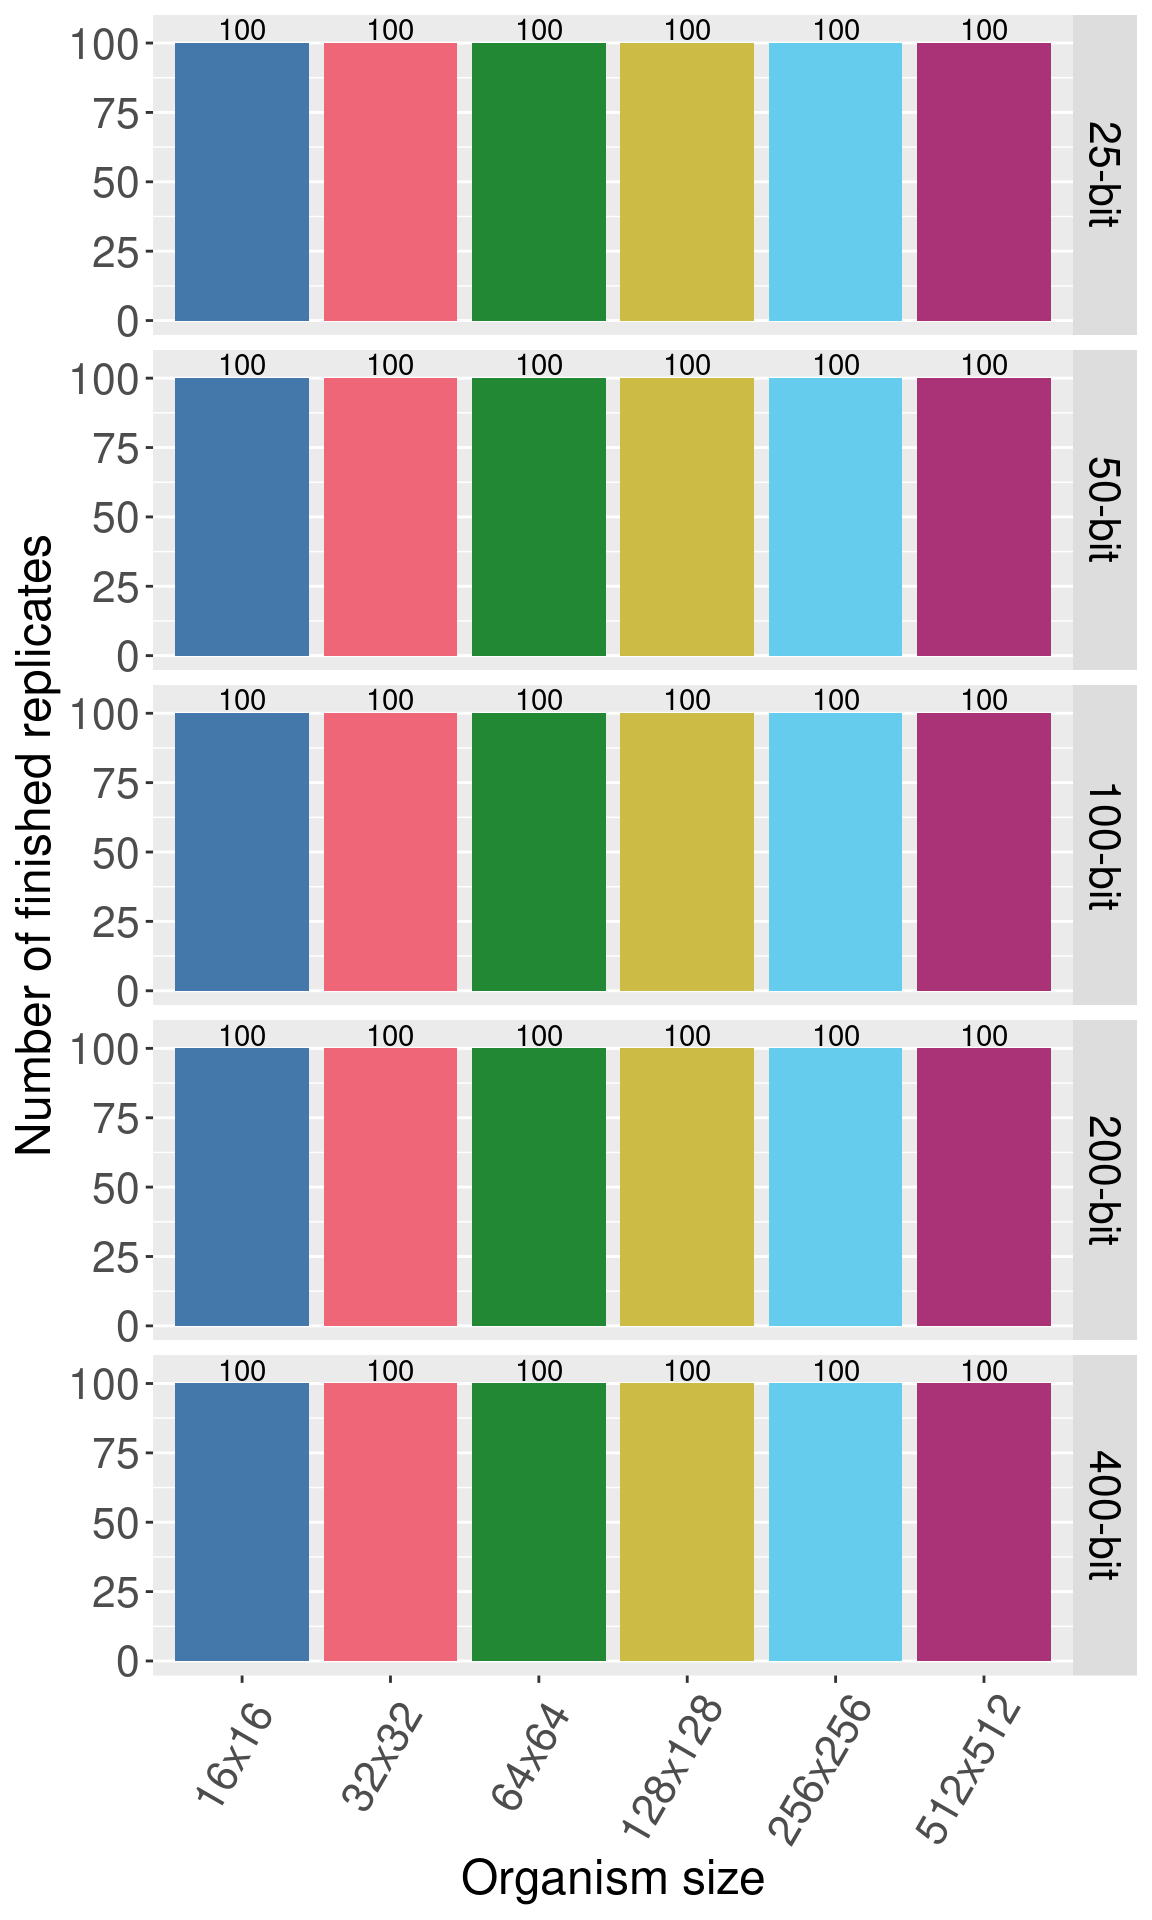
\includegraphics{primordium_supplemental_material_files/figure-latex/unnamed-chunk-62-1.pdf}

\hypertarget{aggregate-plots-3}{%
\section{Aggregate plots}\label{aggregate-plots-3}}

\hypertarget{facet-by-genome-length}{%
\subsection{Facet by genome length}\label{facet-by-genome-length}}

Here we plot all the data at once.
Each row showing a different somatic mutation rate and each boxplot shows a given organism size.

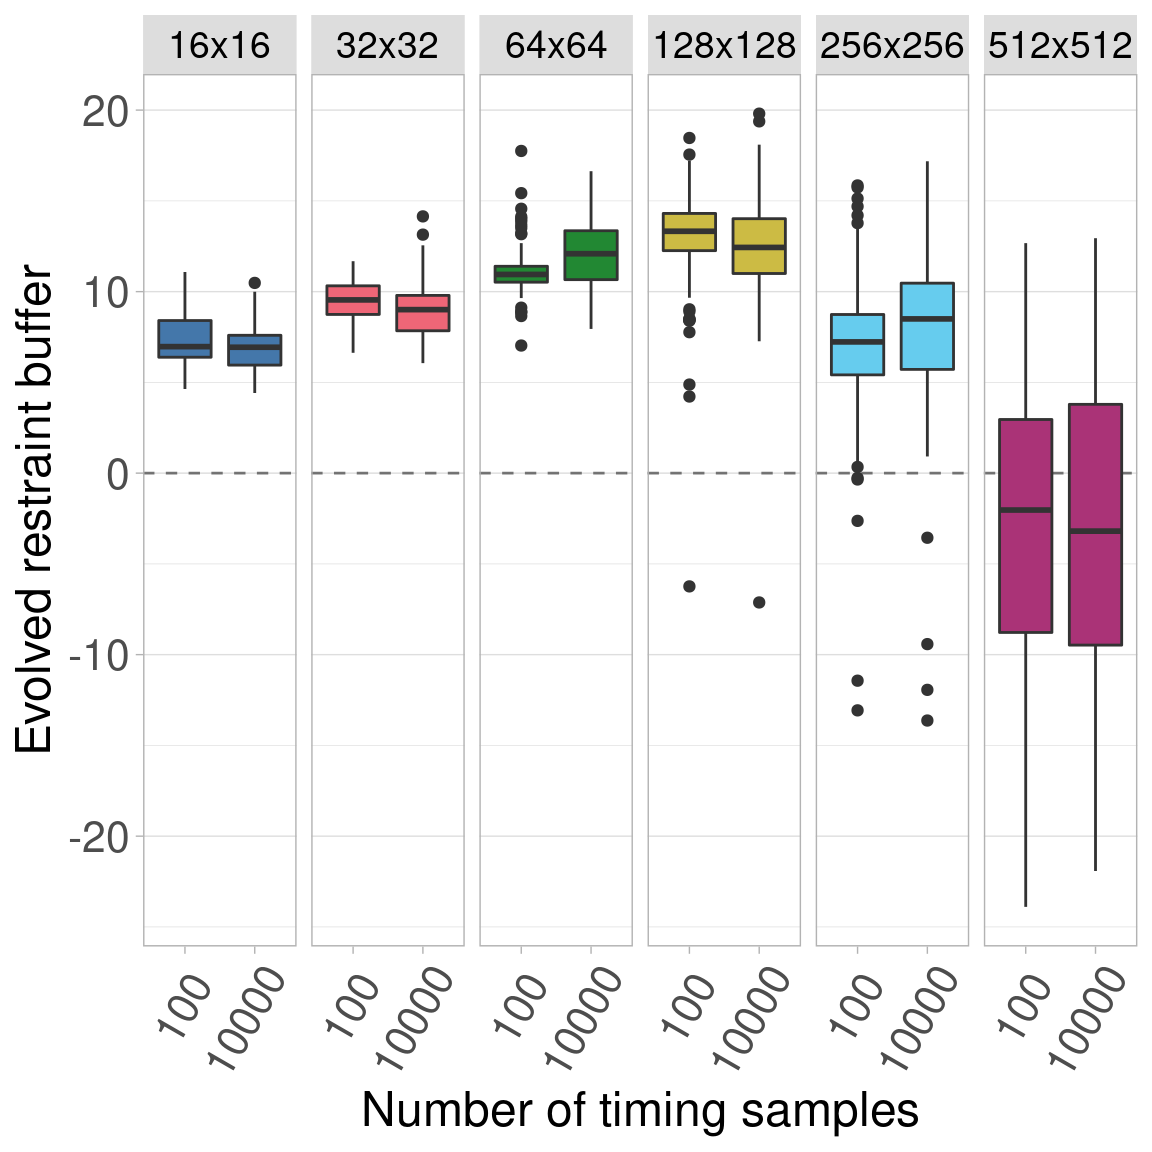
\includegraphics{primordium_supplemental_material_files/figure-latex/unnamed-chunk-63-1.pdf}

Here we plot the same data, only we allow the y-axis to vary between rows.
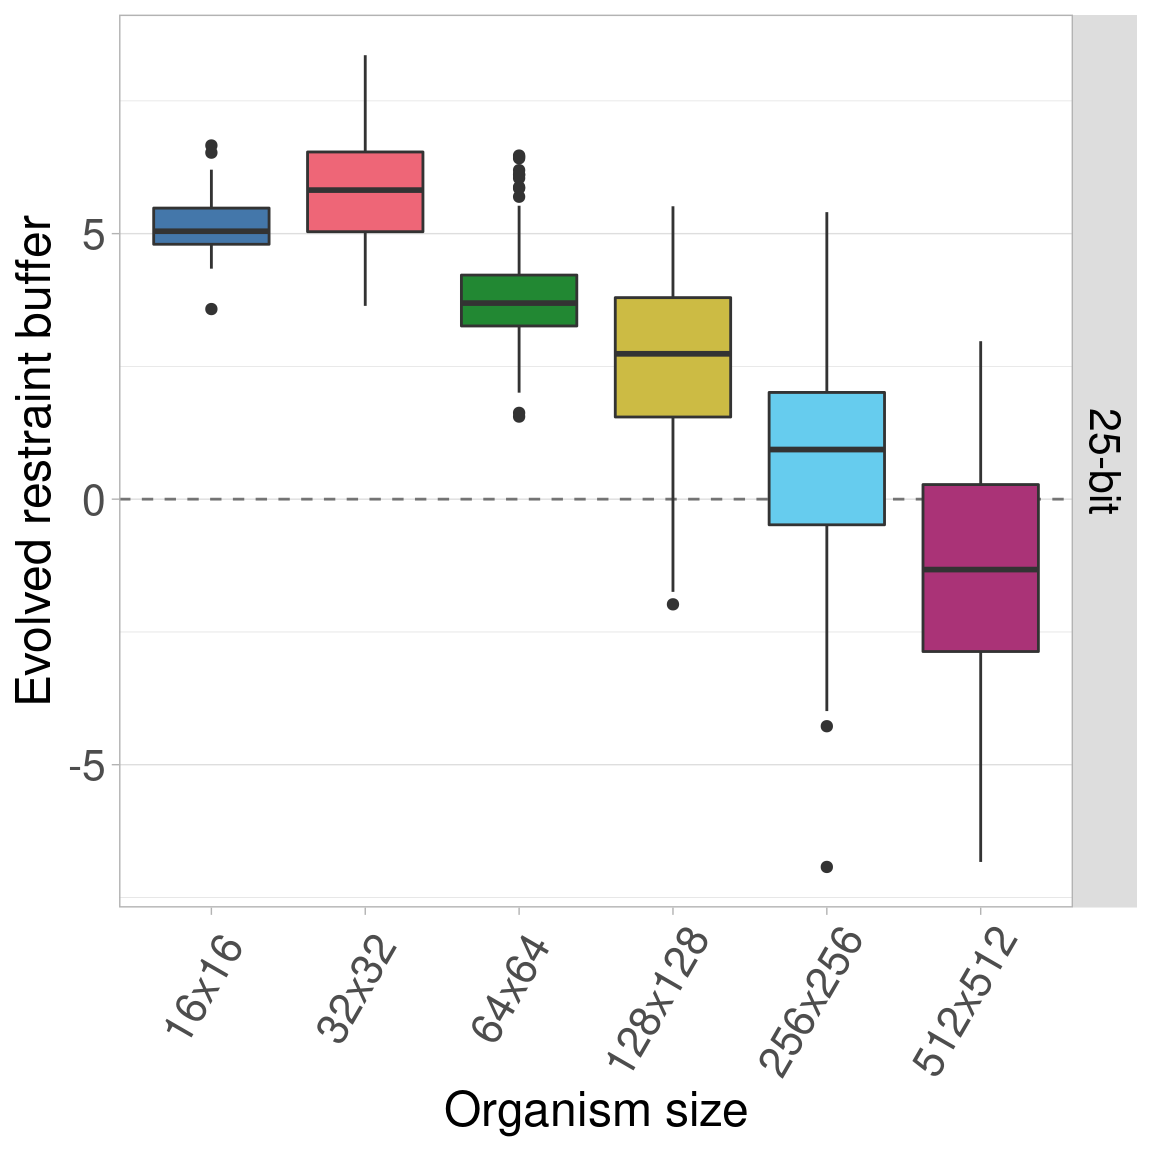
\includegraphics{primordium_supplemental_material_files/figure-latex/unnamed-chunk-64-1.pdf}

\hypertarget{facet-by-organism-size-2}{%
\subsection{Facet by organism size}\label{facet-by-organism-size-2}}

Here we plot the same data again, only now each row shows an organims size while genome length varies on the x-axis.

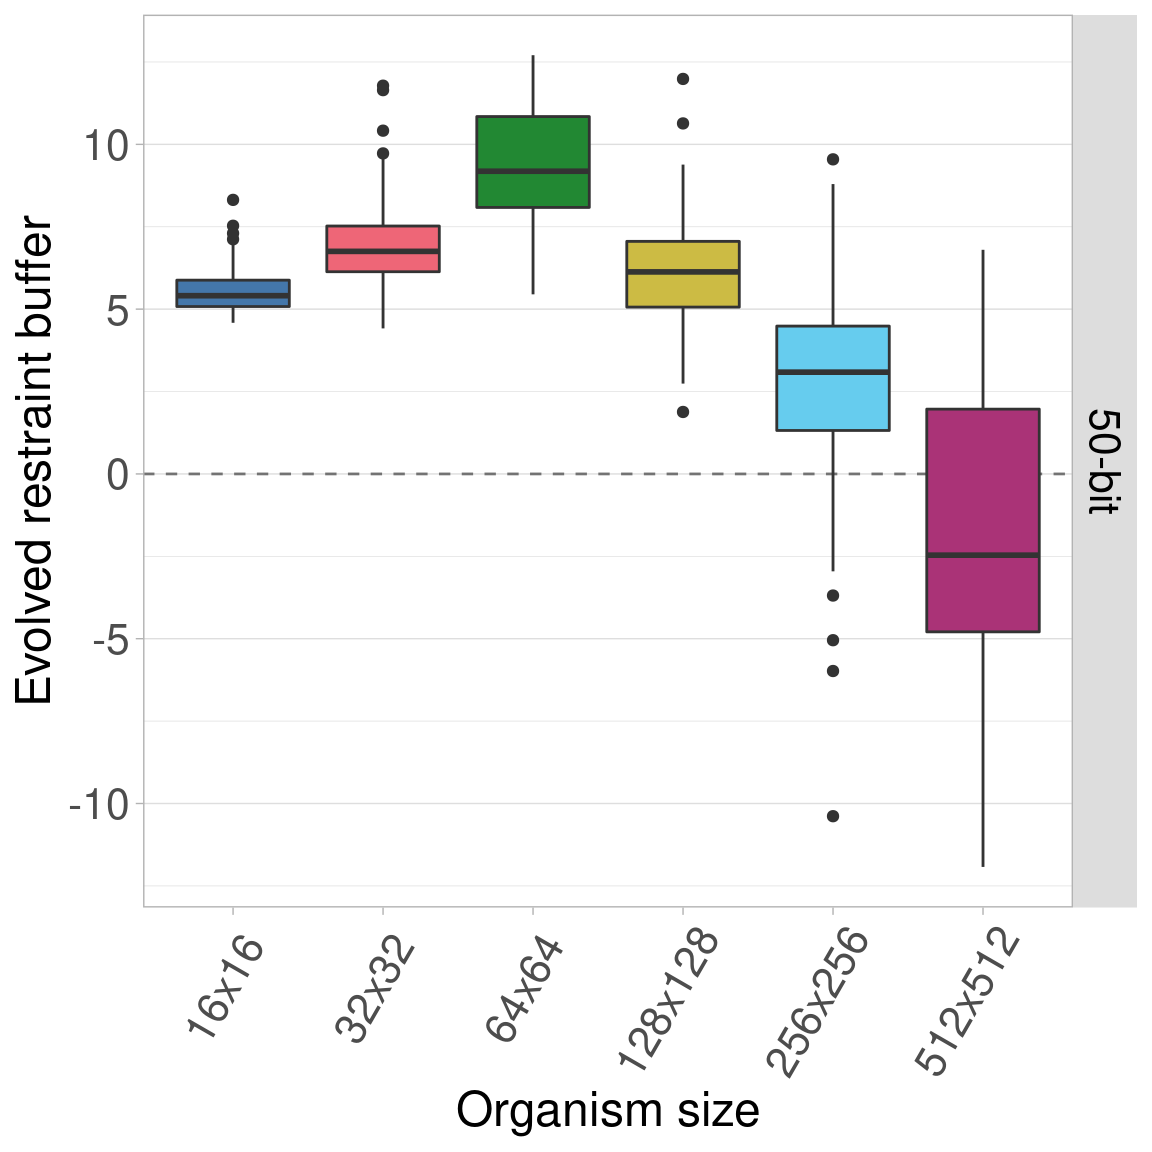
\includegraphics{primordium_supplemental_material_files/figure-latex/unnamed-chunk-65-1.pdf}

Here is the identical plot but now we allow the y-axis to vary between the rows.

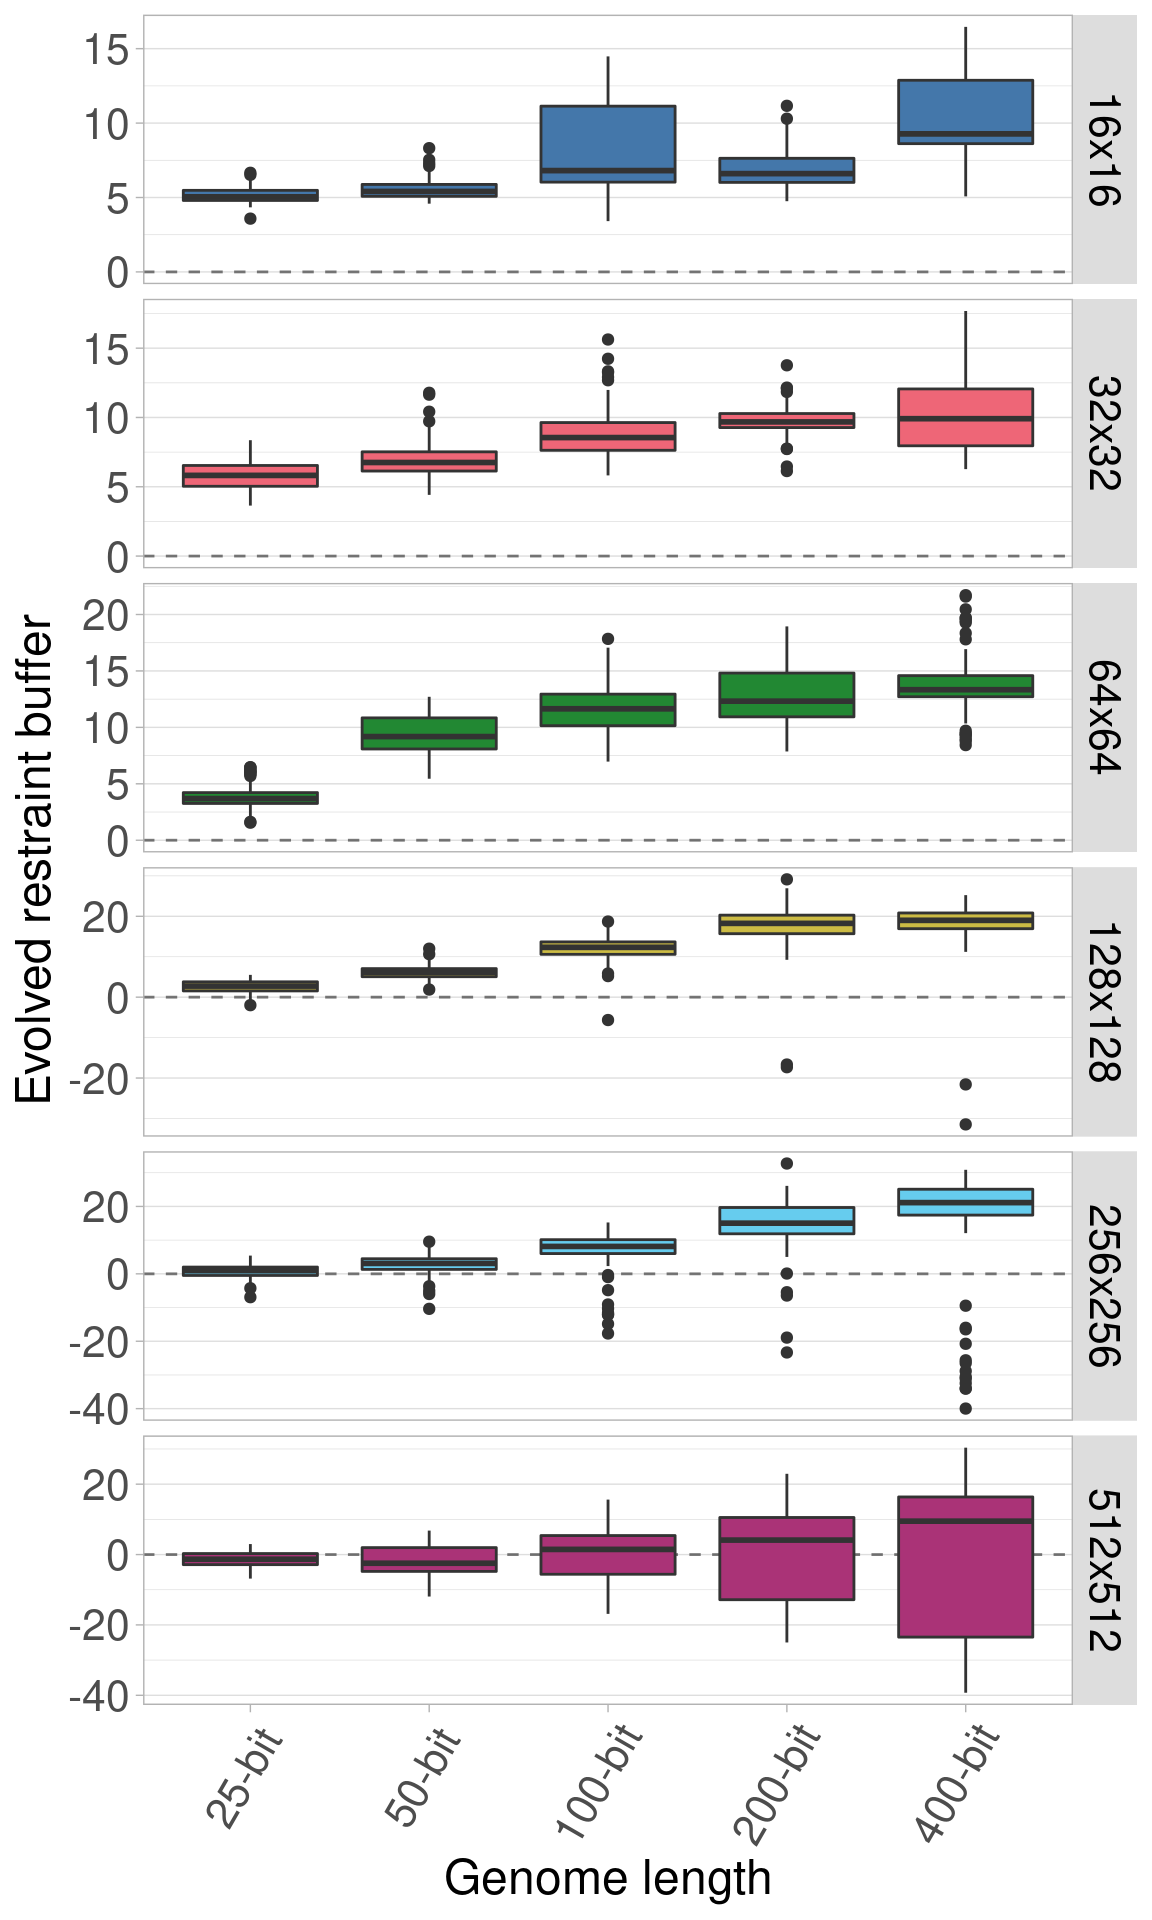
\includegraphics{primordium_supplemental_material_files/figure-latex/unnamed-chunk-66-1.pdf}

\hypertarget{single-organism-size-plots-3}{%
\section{Single organism size plots}\label{single-organism-size-plots-3}}

Here we plot each organism size independently, with the genome length on the x-axis.

\hypertarget{organism-size-16x16-2}{%
\subsection{Organism size 16x16}\label{organism-size-16x16-2}}

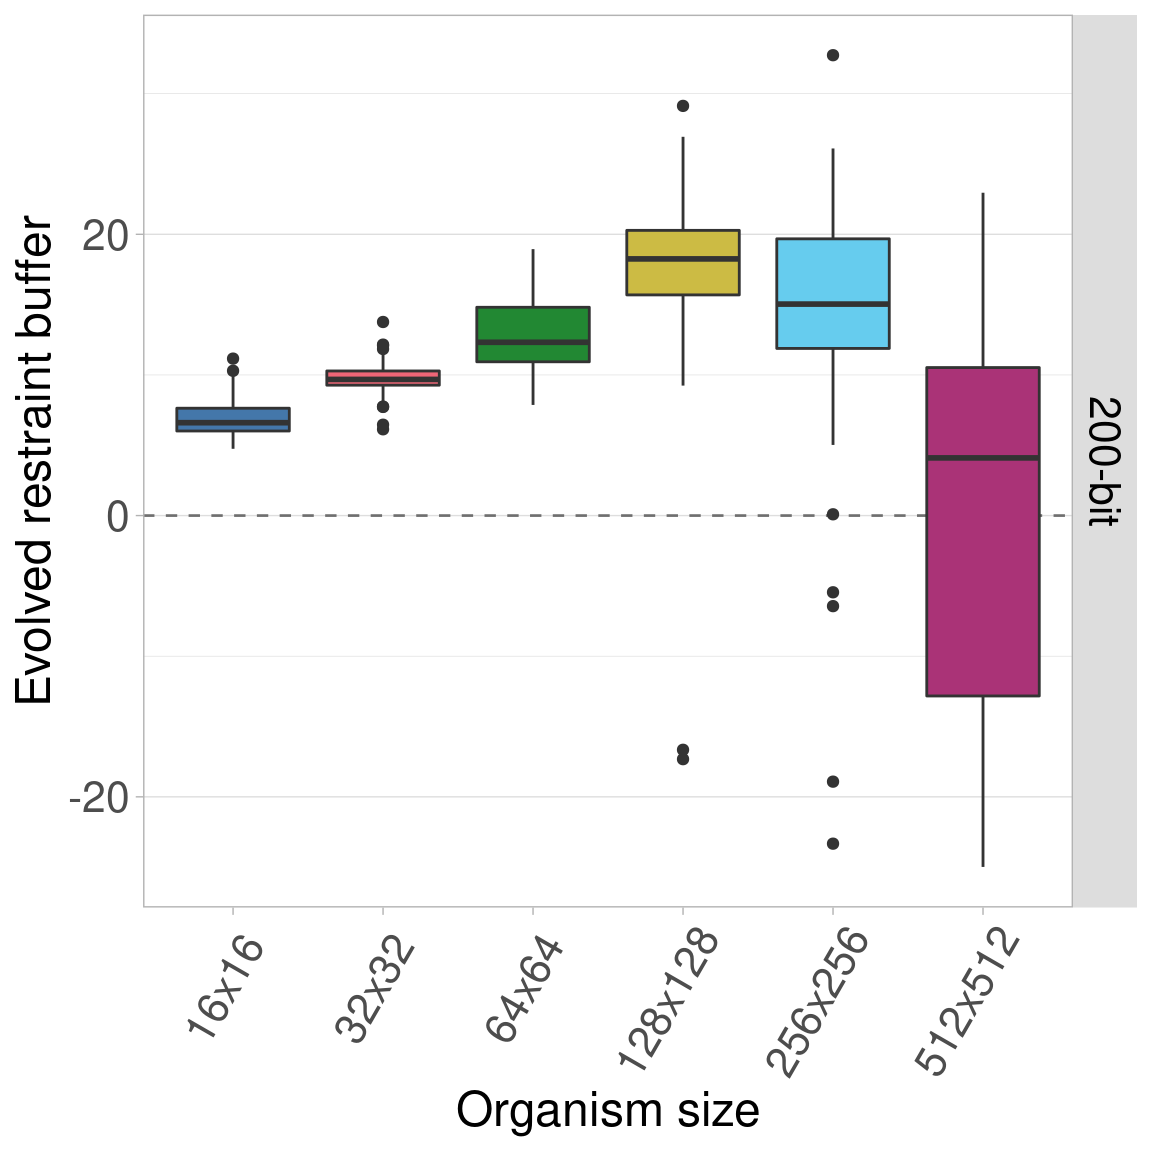
\includegraphics{primordium_supplemental_material_files/figure-latex/unnamed-chunk-67-1.pdf}

\hypertarget{organism-size-32x32-2}{%
\subsection{Organism size 32x32}\label{organism-size-32x32-2}}

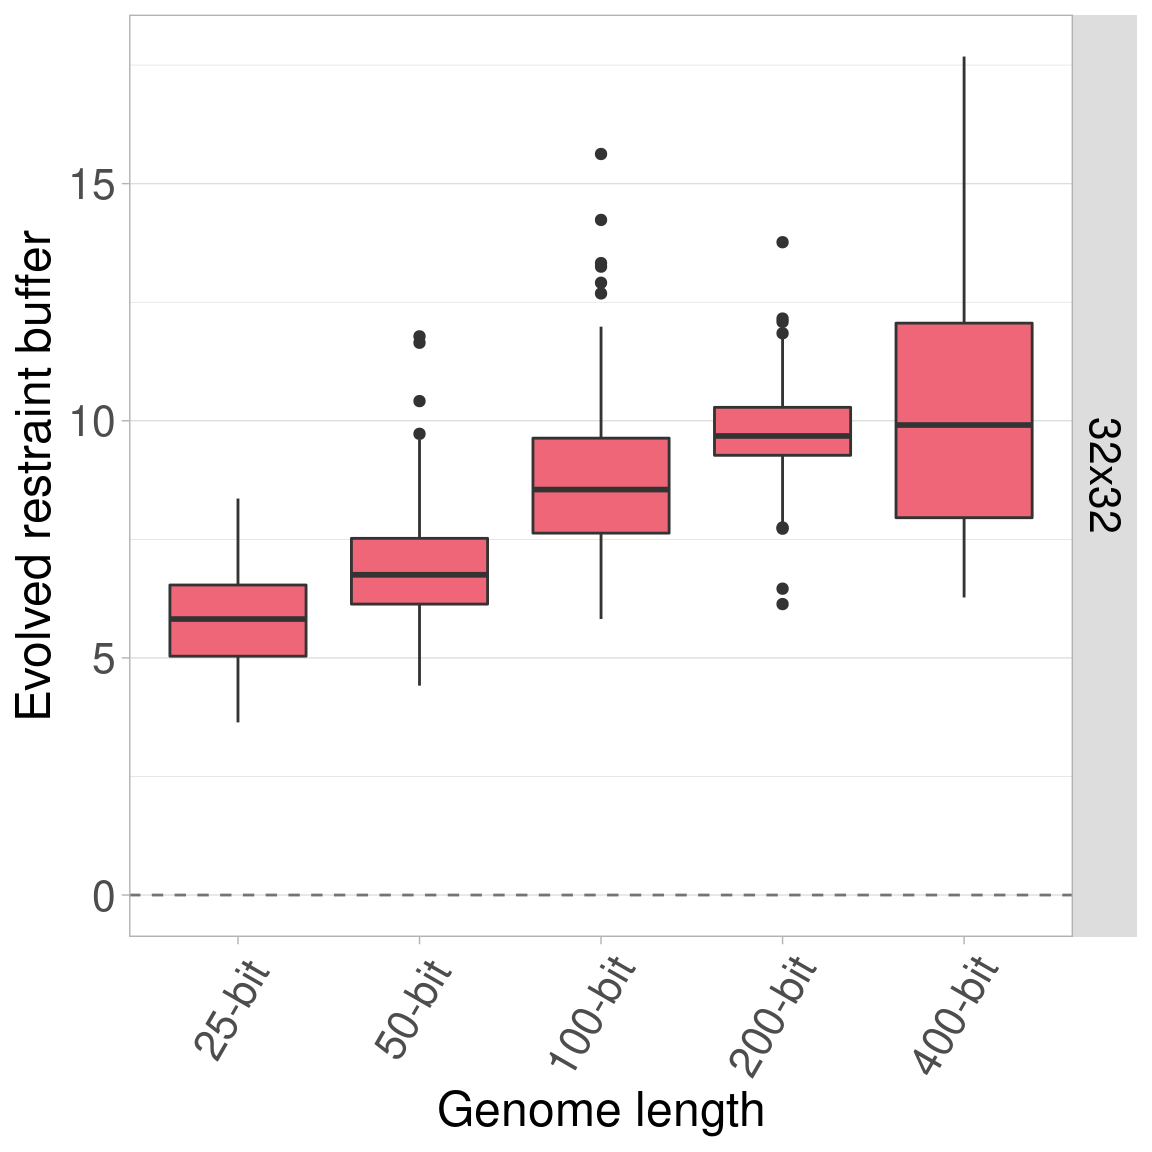
\includegraphics{primordium_supplemental_material_files/figure-latex/unnamed-chunk-68-1.pdf}

\hypertarget{organism-size-64x64-2}{%
\subsection{Organism size 64x64}\label{organism-size-64x64-2}}

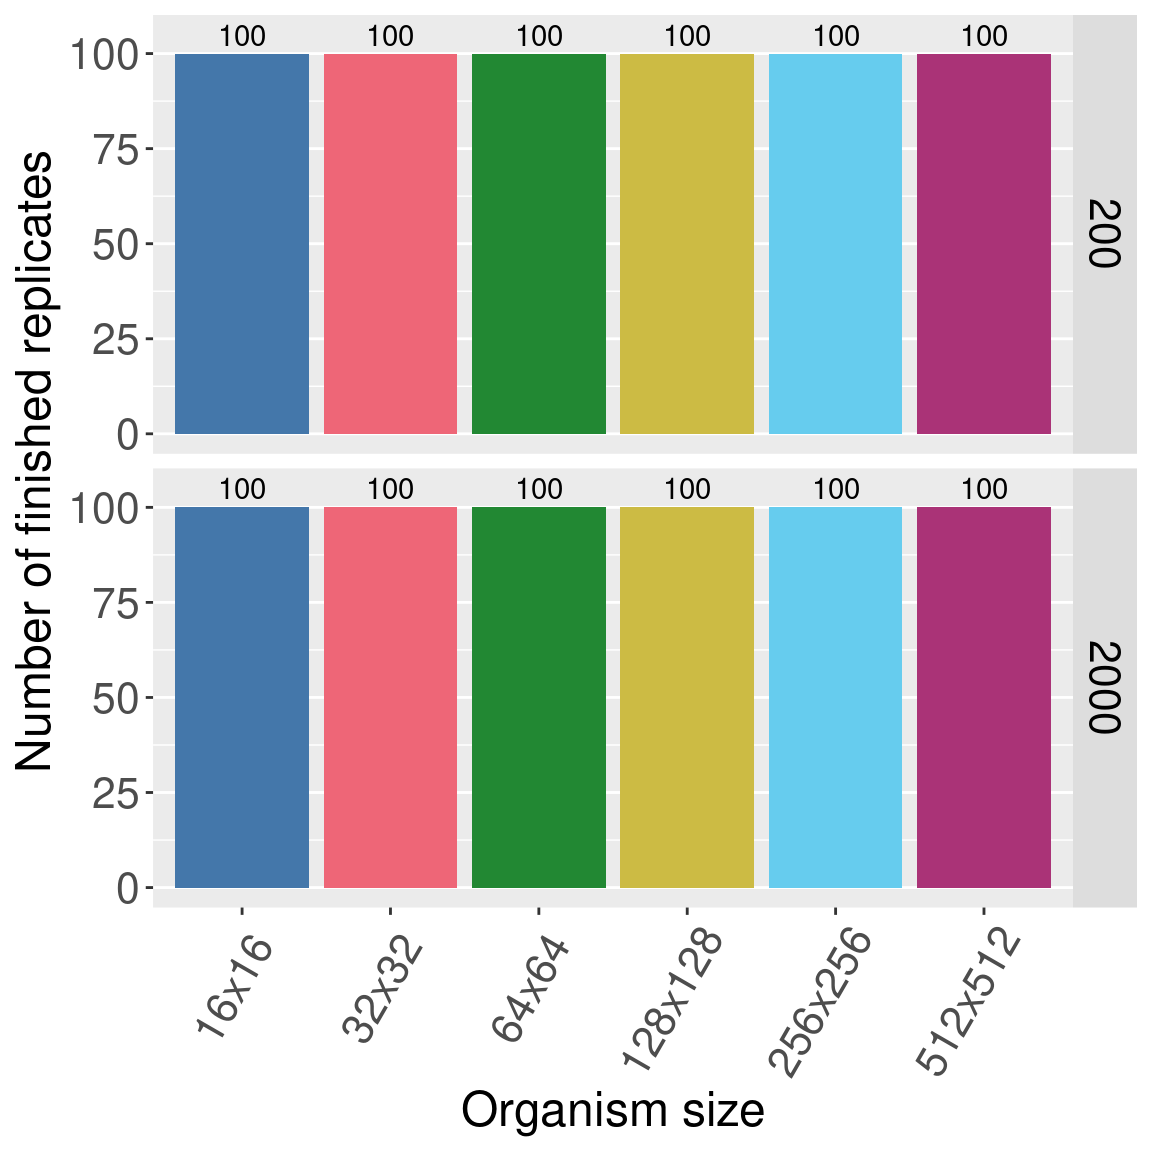
\includegraphics{primordium_supplemental_material_files/figure-latex/unnamed-chunk-69-1.pdf}

\hypertarget{organism-size-128x128-2}{%
\subsection{Organism size 128x128}\label{organism-size-128x128-2}}

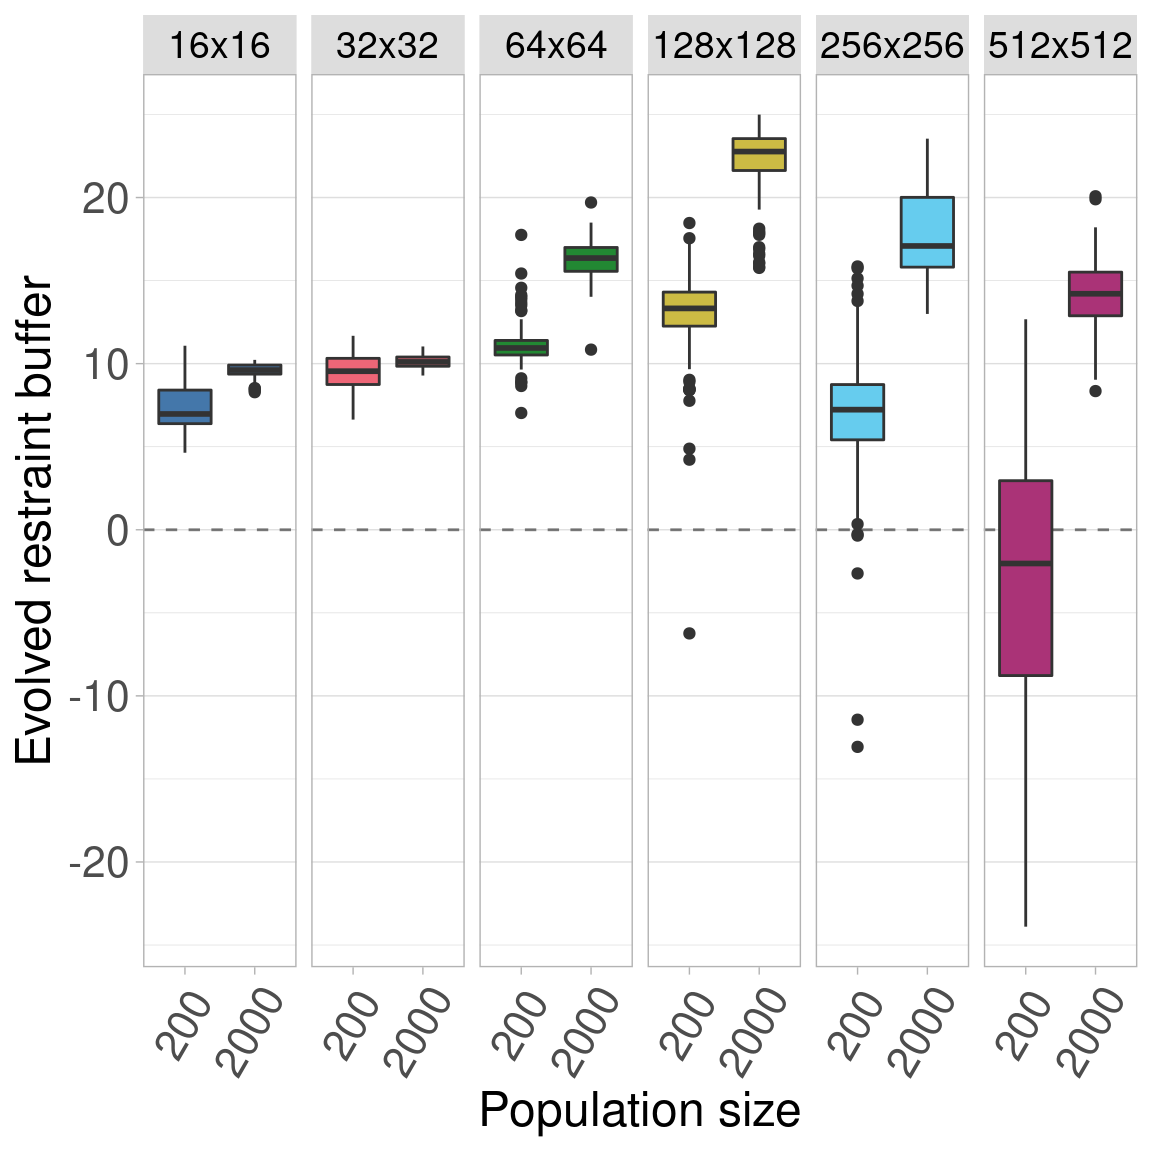
\includegraphics{primordium_supplemental_material_files/figure-latex/unnamed-chunk-70-1.pdf}

\hypertarget{organism-size-256x256-2}{%
\subsection{Organism size 256x256}\label{organism-size-256x256-2}}

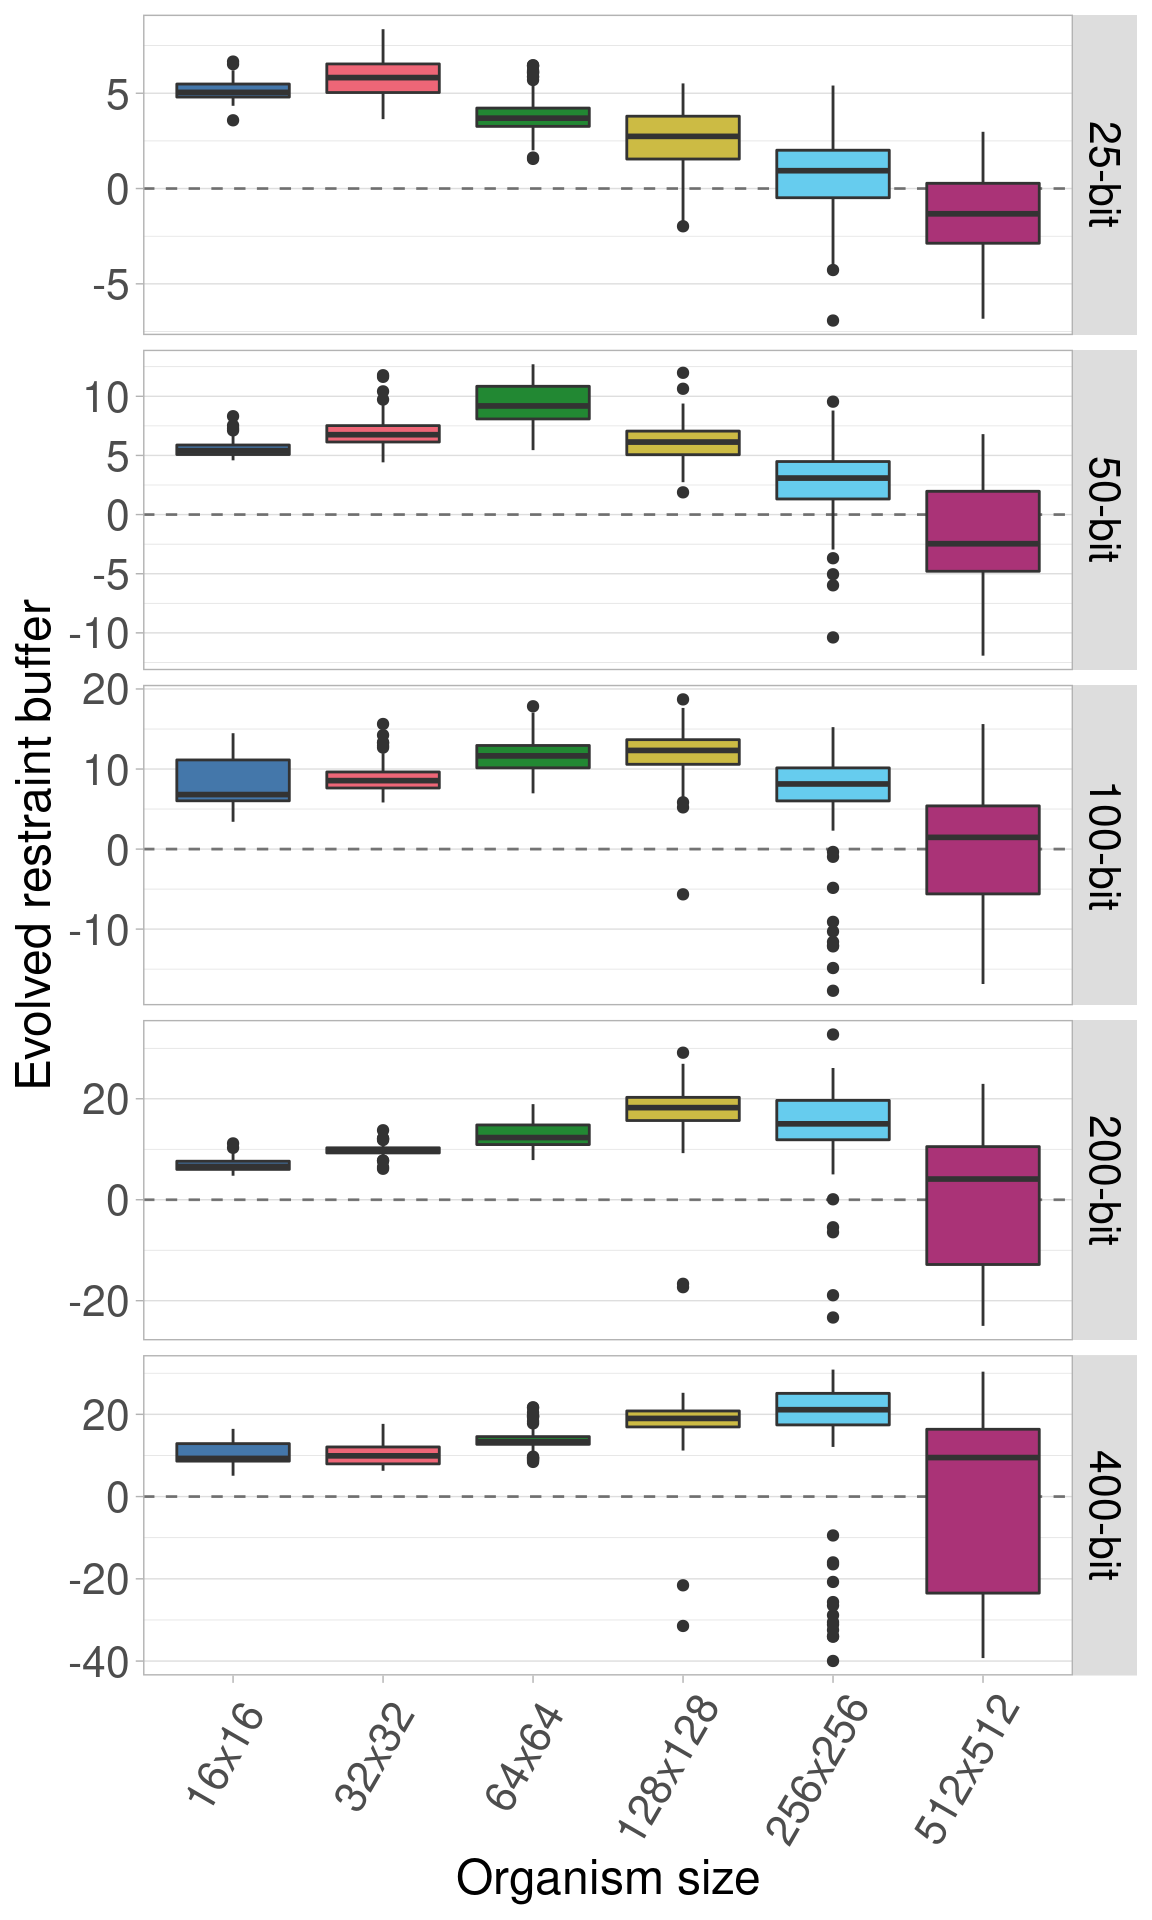
\includegraphics{primordium_supplemental_material_files/figure-latex/unnamed-chunk-71-1.pdf}

\hypertarget{organism-size-512x512-2}{%
\subsection{Organism size 512x512}\label{organism-size-512x512-2}}

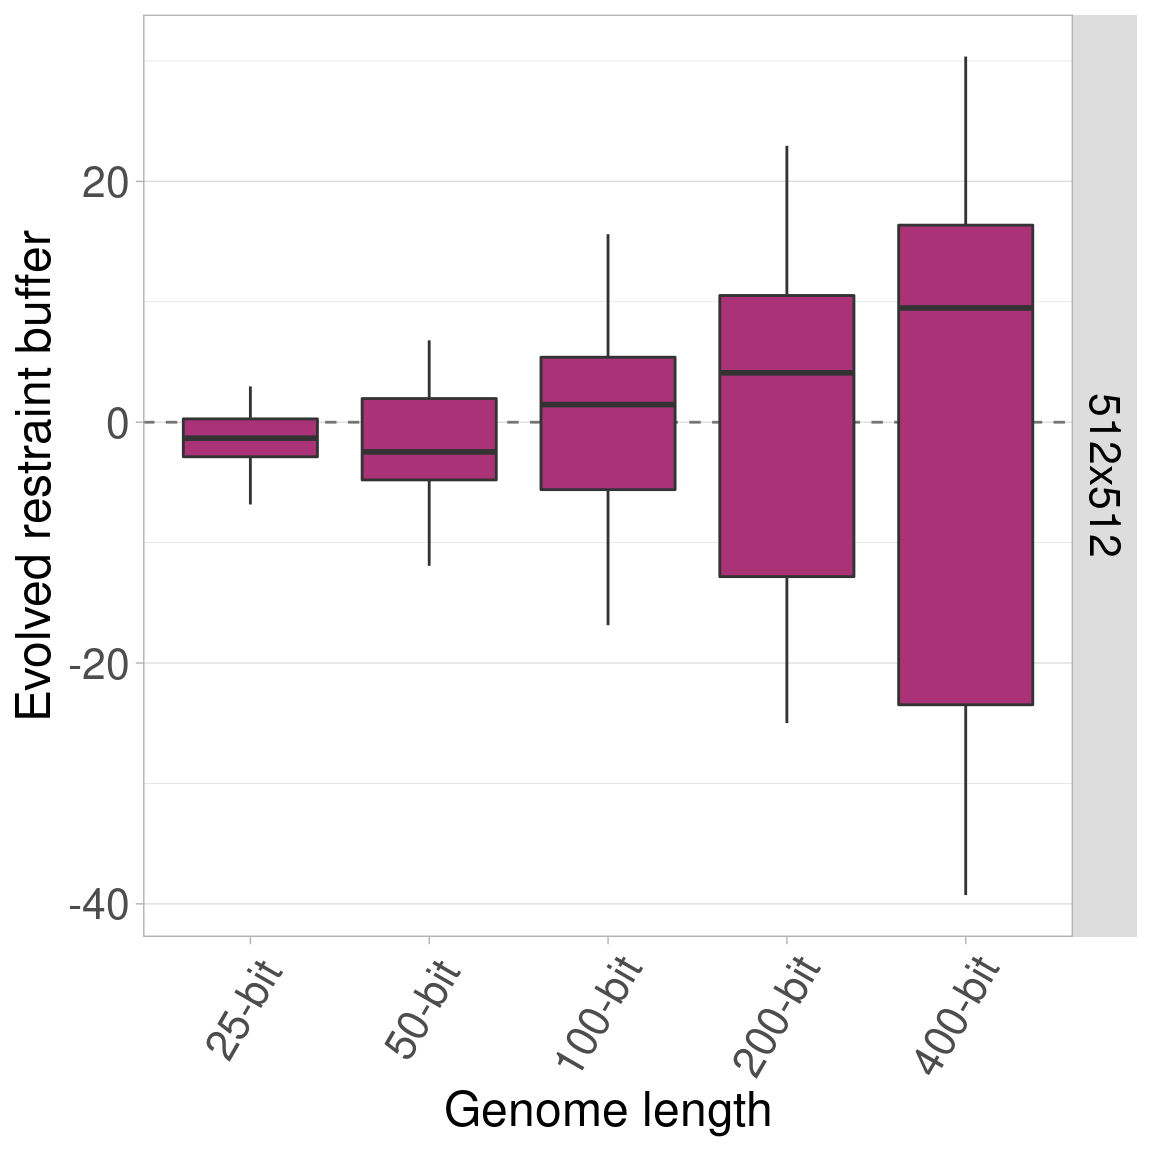
\includegraphics{primordium_supplemental_material_files/figure-latex/unnamed-chunk-72-1.pdf}

\hypertarget{single-genome-length-plots}{%
\section{Single genome length plots}\label{single-genome-length-plots}}

Here we plot each genome length independently, with the organism size on the x-axis.

\hypertarget{bit-genomes}{%
\subsection{25-bit genomes}\label{bit-genomes}}

\includegraphics{primordium_supplemental_material_files/figure-latex/unnamed-chunk-73-1.pdf}

\hypertarget{bit-genomes-1}{%
\subsection{50-bit genomes}\label{bit-genomes-1}}

\includegraphics{primordium_supplemental_material_files/figure-latex/unnamed-chunk-74-1.pdf}

\hypertarget{bit-genomes-2}{%
\subsection{100-bit genomes}\label{bit-genomes-2}}

\includegraphics{primordium_supplemental_material_files/figure-latex/unnamed-chunk-75-1.pdf}

\hypertarget{bit-genomes-3}{%
\subsection{200-bit genomes}\label{bit-genomes-3}}

\includegraphics{primordium_supplemental_material_files/figure-latex/unnamed-chunk-76-1.pdf}

\hypertarget{bit-genomes-4}{%
\subsection{400-bit genomes}\label{bit-genomes-4}}

\includegraphics{primordium_supplemental_material_files/figure-latex/unnamed-chunk-77-1.pdf}

\hypertarget{statistics-3}{%
\section{Statistics}\label{statistics-3}}

Since organism size is our main point of comparison, we calculate stats for each genome length.

First, we perform a Kruskal-Wallis test across all organism sizes to indicate if variance exists at that mutation rate.
If variance exists, we then perfrm a pairwise Wilcoxon Rank-Sum test to show which pairs of organism sizes significantly differ.
Finally, we perform Bonferroni-Holm corrections for multiple comparisons.

\begin{Shaded}
\begin{Highlighting}[]
\NormalTok{  length_vec =}\StringTok{ }\KeywordTok{c}\NormalTok{(}\DecValTok{25}\NormalTok{, }\DecValTok{50}\NormalTok{, }\DecValTok{100}\NormalTok{, }\DecValTok{200}\NormalTok{, }\DecValTok{400}\NormalTok{)}
\NormalTok{  df_kruskal =}\StringTok{ }\KeywordTok{data.frame}\NormalTok{(}\DataTypeTok{data =} \KeywordTok{matrix}\NormalTok{(}\DataTypeTok{nrow =} \DecValTok{0}\NormalTok{, }\DataTypeTok{ncol =} \DecValTok{4}\NormalTok{))}
  \KeywordTok{colnames}\NormalTok{(df_kruskal) =}\StringTok{ }\KeywordTok{c}\NormalTok{(}\StringTok{'genome_length'}\NormalTok{, }\StringTok{'p_value'}\NormalTok{, }\StringTok{'chi_squared'}\NormalTok{, }\StringTok{'df'}\NormalTok{)}
  \ControlFlowTok{for}\NormalTok{(genome_length }\ControlFlowTok{in}\NormalTok{ length_vec)\{}
\NormalTok{    df_test =}\StringTok{ }\NormalTok{df2[df2}\OperatorTok{$}\NormalTok{LENGTH }\OperatorTok{==}\StringTok{ }\NormalTok{genome_length,]}
\NormalTok{    res =}\StringTok{ }\KeywordTok{kruskal.test}\NormalTok{(df_test}\OperatorTok{$}\NormalTok{restraint_value }\OperatorTok{~}\StringTok{ }\NormalTok{df_test}\OperatorTok{$}\NormalTok{MCSIZE, df_test)}
\NormalTok{    df_kruskal[}\KeywordTok{nrow}\NormalTok{(df_kruskal) }\OperatorTok{+}\StringTok{ }\DecValTok{1}\NormalTok{,] =}\StringTok{ }\KeywordTok{c}\NormalTok{(genome_length, res}\OperatorTok{$}\NormalTok{p.value, }\KeywordTok{as.numeric}\NormalTok{(res}\OperatorTok{$}\NormalTok{statistic)[}\DecValTok{1}\NormalTok{], }\KeywordTok{as.numeric}\NormalTok{(res}\OperatorTok{$}\NormalTok{parameter)[}\DecValTok{1}\NormalTok{])}
\NormalTok{  \}}
\NormalTok{  df_kruskal}\OperatorTok{$}\NormalTok{less_}\FloatTok{0.01}\NormalTok{ =}\StringTok{ }\NormalTok{df_kruskal}\OperatorTok{$}\NormalTok{p_value }\OperatorTok{<}\StringTok{ }\FloatTok{0.01}
  \KeywordTok{print}\NormalTok{(df_kruskal)}
\end{Highlighting}
\end{Shaded}

\begin{verbatim}
##   genome_length      p_value chi_squared df less_0.01
## 1            25 1.508889e-97    461.6473  5      TRUE
## 2            50 9.772852e-87    411.5159  5      TRUE
## 3           100 7.491319e-60    286.6294  5      TRUE
## 4           200 1.626963e-75    359.4358  5      TRUE
## 5           400 2.857912e-49    237.3380  5      TRUE
\end{verbatim}

We see that significant variation exists within each genome length, so we perform pariwise Wilcoxon tests on each to see which pais of sizes are significantly different.

\begin{Shaded}
\begin{Highlighting}[]
\NormalTok{size_vec =}\StringTok{ }\KeywordTok{c}\NormalTok{(}\DecValTok{16}\NormalTok{, }\DecValTok{32}\NormalTok{, }\DecValTok{64}\NormalTok{, }\DecValTok{128}\NormalTok{, }\DecValTok{256}\NormalTok{, }\DecValTok{512}\NormalTok{)}
\NormalTok{length_vec =}\StringTok{ }\KeywordTok{c}\NormalTok{(}\DecValTok{25}\NormalTok{, }\DecValTok{50}\NormalTok{, }\DecValTok{100}\NormalTok{, }\DecValTok{200}\NormalTok{, }\DecValTok{400}\NormalTok{)}
\ControlFlowTok{for}\NormalTok{(genome_length }\ControlFlowTok{in}\NormalTok{ length_vec)\{}
\NormalTok{  df_test =}\StringTok{ }\NormalTok{df2[df2}\OperatorTok{$}\NormalTok{LENGTH }\OperatorTok{==}\StringTok{ }\NormalTok{genome_length,]}
\NormalTok{  df_wilcox =}\StringTok{ }\KeywordTok{data.frame}\NormalTok{(}\DataTypeTok{data =} \KeywordTok{matrix}\NormalTok{(}\DataTypeTok{nrow =} \DecValTok{0}\NormalTok{, }\DataTypeTok{ncol =} \DecValTok{6}\NormalTok{))}
  \KeywordTok{colnames}\NormalTok{(df_wilcox) =}\StringTok{ }\KeywordTok{c}\NormalTok{(}\StringTok{'genome_length'}\NormalTok{, }\StringTok{'size_a'}\NormalTok{, }\StringTok{'size_b'}\NormalTok{, }\StringTok{'p_value_corrected'}\NormalTok{, }\StringTok{'p_value_raw'}\NormalTok{, }\StringTok{'W'}\NormalTok{)}
  \ControlFlowTok{for}\NormalTok{(size_idx_a }\ControlFlowTok{in} \DecValTok{1}\OperatorTok{:}\NormalTok{(}\KeywordTok{length}\NormalTok{(size_vec) }\OperatorTok{-}\StringTok{ }\DecValTok{1}\NormalTok{))\{}
\NormalTok{    size_a =}\StringTok{ }\NormalTok{size_vec[size_idx_a]}
    \ControlFlowTok{for}\NormalTok{(size_idx_b }\ControlFlowTok{in}\NormalTok{ (size_idx_a }\OperatorTok{+}\StringTok{ }\DecValTok{1}\NormalTok{)}\OperatorTok{:}\KeywordTok{length}\NormalTok{(size_vec))\{}
\NormalTok{      size_b =}\StringTok{ }\NormalTok{size_vec[size_idx_b]}
\NormalTok{      res =}\StringTok{ }\KeywordTok{wilcox.test}\NormalTok{(df_test[df_test}\OperatorTok{$}\NormalTok{MCSIZE }\OperatorTok{==}\StringTok{ }\NormalTok{size_a,]}\OperatorTok{$}\NormalTok{restraint_value, df_test[df_test}\OperatorTok{$}\NormalTok{MCSIZE }\OperatorTok{==}\StringTok{ }\NormalTok{size_b,]}\OperatorTok{$}\NormalTok{restraint_value, }\DataTypeTok{alternative =} \StringTok{'two.sided'}\NormalTok{) }
\NormalTok{      df_wilcox[}\KeywordTok{nrow}\NormalTok{(df_wilcox) }\OperatorTok{+}\StringTok{ }\DecValTok{1}\NormalTok{,] =}\StringTok{ }\KeywordTok{c}\NormalTok{(genome_length, size_a, size_b, }\DecValTok{0}\NormalTok{, res}\OperatorTok{$}\NormalTok{p.value, }\KeywordTok{as.numeric}\NormalTok{(res}\OperatorTok{$}\NormalTok{statistic)[}\DecValTok{1}\NormalTok{])}
\NormalTok{    \}}
\NormalTok{  \}}
\NormalTok{  df_wilcox}\OperatorTok{$}\NormalTok{p_value_corrected =}\StringTok{ }\KeywordTok{p.adjust}\NormalTok{(df_wilcox}\OperatorTok{$}\NormalTok{p_value_raw, }\DataTypeTok{method =} \StringTok{'holm'}\NormalTok{)}
\NormalTok{  df_wilcox}\OperatorTok{$}\NormalTok{less_}\FloatTok{0.01}\NormalTok{ =}\StringTok{ }\NormalTok{df_wilcox}\OperatorTok{$}\NormalTok{p_value_corrected }\OperatorTok{<}\StringTok{ }\FloatTok{0.01}
  \KeywordTok{print}\NormalTok{(}\KeywordTok{paste0}\NormalTok{(}\StringTok{'Genome length: '}\NormalTok{, genome_length))}
  \KeywordTok{print}\NormalTok{(df_wilcox)}
\NormalTok{\}}
\end{Highlighting}
\end{Shaded}

\begin{verbatim}
## [1] "Genome length: 25"
##    genome_length size_a size_b p_value_corrected  p_value_raw       W less_0.01
## 1             25     16     32      2.337475e-07 2.337475e-07  2883.5      TRUE
## 2             25     16     64      6.069986e-18 1.213997e-18  8607.5      TRUE
## 3             25     16    128      1.663209e-24 2.376012e-25  9258.5      TRUE
## 4             25     16    256      6.203828e-32 5.639844e-33  9896.0      TRUE
## 5             25     16    512      3.838888e-33 2.559259e-34 10000.0      TRUE
## 6             25     32     64      1.447210e-22 2.412016e-23  9074.5      TRUE
## 7             25     32    128      1.283820e-27 1.283820e-28  9542.5      TRUE
## 8             25     32    256      2.711275e-32 2.259396e-33  9927.0      TRUE
## 9             25     32    512      3.838888e-33 2.560557e-34 10000.0      TRUE
## 10            25     64    128      1.187343e-07 5.936715e-08  7219.0      TRUE
## 11            25     64    256      2.378014e-26 2.642238e-27  9430.5      TRUE
## 12            25     64    512      1.298354e-32 9.987336e-34  9954.5      TRUE
## 13            25    128    256      1.433015e-10 3.582536e-11  7710.0      TRUE
## 14            25    128    512      7.524923e-25 9.406154e-26  9294.5      TRUE
## 15            25    256    512      4.120336e-10 1.373445e-10  7627.5      TRUE
## [1] "Genome length: 50"
##    genome_length size_a size_b p_value_corrected  p_value_raw      W less_0.01
## 1             50     16     32      2.588989e-15 5.177978e-16 1681.5      TRUE
## 2             50     16     64      2.694326e-30 2.072558e-31  228.0      TRUE
## 3             50     16    128      3.224011e-03 3.224011e-03 3794.0      TRUE
## 4             50     16    256      4.089878e-15 1.022470e-15 8284.5      TRUE
## 5             50     16    512      1.182991e-27 1.182991e-28 9545.5      TRUE
## 6             50     32     64      1.797027e-17 2.567181e-18 1427.0      TRUE
## 7             50     32    128      7.415731e-04 3.707866e-04 6457.5      TRUE
## 8             50     32    256      1.165570e-21 1.295078e-22 9005.5      TRUE
## 9             50     32    512      4.567933e-31 3.262810e-32 9836.0      TRUE
## 10            50     64    128      2.265727e-21 2.832159e-22 8973.0      TRUE
## 11            50     64    256      8.866606e-30 7.388839e-31 9727.5      TRUE
## 12            50     64    512      7.213069e-33 4.808713e-34 9979.0      TRUE
## 13            50    128    256      4.869262e-16 8.115436e-17 8409.5      TRUE
## 14            50    128    512      4.777498e-28 4.343180e-29 9582.0      TRUE
## 15            50    256    512      3.236734e-12 1.078911e-12 7914.5      TRUE
## [1] "Genome length: 100"
##    genome_length size_a size_b p_value_corrected  p_value_raw      W less_0.01
## 1            100     16     32      7.697389e-02 1.924347e-02 4041.5     FALSE
## 2            100     16     64      3.952168e-13 7.904337e-14 1941.5      TRUE
## 3            100     16    128      2.398968e-14 2.998710e-15 1770.0      TRUE
## 4            100     16    256      4.158441e-01 4.158441e-01 5333.5     FALSE
## 5            100     16    512      5.614119e-18 4.678432e-19 8651.0      TRUE
## 6            100     32     64      1.034976e-13 1.478537e-14 1852.5      TRUE
## 7            100     32    128      3.085548e-17 3.085548e-18 1435.5      TRUE
## 8            100     32    256      1.117541e-01 3.725137e-02 5853.0     FALSE
## 9            100     32    512      2.483010e-22 1.910008e-23 9084.0      TRUE
## 10           100     64    128      1.117541e-01 4.890986e-02 4193.5     FALSE
## 11           100     64    256      5.002561e-15 5.558401e-16 8315.0      TRUE
## 12           100     64    512      5.082595e-28 3.388396e-29 9591.0      TRUE
## 13           100    128    256      1.590814e-17 1.446195e-18 8599.5      TRUE
## 14           100    128    512      9.444159e-28 6.745828e-29 9566.0      TRUE
## 15           100    256    512      2.634367e-13 4.390611e-14 8090.0      TRUE
## [1] "Genome length: 200"
##    genome_length size_a size_b p_value_corrected  p_value_raw      W less_0.01
## 1            200     16     32      4.663546e-26 3.886289e-27  584.0      TRUE
## 2            200     16     64      7.523609e-32 5.015739e-33  100.0      TRUE
## 3            200     16    128      2.146093e-30 1.532923e-31  217.5      TRUE
## 4            200     16    256      1.997886e-24 1.911300e-25  733.0      TRUE
## 5            200     16    512      9.462181e-03 9.462181e-03 6062.5      TRUE
## 6            200     32     64      1.344008e-20 1.493343e-21 1097.0      TRUE
## 7            200     32    128      5.645064e-28 4.342357e-29  418.0      TRUE
## 8            200     32    256      1.309572e-19 1.636965e-20 1200.0      TRUE
## 9            200     32    512      2.440723e-07 6.101808e-08 7217.0      TRUE
## 10           200     64    128      1.166719e-18 1.666742e-19 1302.5      TRUE
## 11           200     64    256      9.151807e-05 3.050602e-05 3293.0      TRUE
## 12           200     64    512      6.237644e-15 1.247529e-15 8274.5      TRUE
## 13           200    128    256      9.982635e-05 4.991318e-05 6660.5      TRUE
## 14           200    128    512      1.997886e-24 1.816260e-25 9269.0      TRUE
## 15           200    256    512      1.717006e-17 2.861676e-18 8568.0      TRUE
## [1] "Genome length: 400"
##    genome_length size_a size_b p_value_corrected  p_value_raw      W less_0.01
## 1            400     16     32      5.405382e-01 5.348472e-01 5254.5     FALSE
## 2            400     16     64      3.472338e-14 3.472338e-15 1777.5      TRUE
## 3            400     16    128      4.072814e-28 2.715209e-29  401.0      TRUE
## 4            400     16    256      1.163125e-16 9.692706e-18 1489.0      TRUE
## 5            400     16    512      5.405382e-01 1.801794e-01 5549.0     FALSE
## 6            400     32     64      5.784416e-12 8.263451e-13 2070.5      TRUE
## 7            400     32    128      1.489024e-26 1.063588e-27  535.5      TRUE
## 8            400     32    256      2.187697e-16 1.988815e-17 1523.0      TRUE
## 9            400     32    512      5.405382e-01 1.825748e-01 5546.0     FALSE
## 10           400     64    128      2.993077e-18 2.302367e-19 1317.0      TRUE
## 11           400     64    256      3.197608e-12 3.997010e-13 2030.0      TRUE
## 12           400     64    512      8.293488e-05 1.658698e-05 6763.0      TRUE
## 13           400    128    256      1.019174e-02 2.547935e-03 3764.5     FALSE
## 14           400    128    512      9.137039e-13 1.015227e-13 8045.0      TRUE
## 15           400    256    512      6.084030e-12 1.014005e-12 7918.0      TRUE
\end{verbatim}

\hypertarget{test-of-timing-sample-counts}{%
\chapter{Test of timing sample counts}\label{test-of-timing-sample-counts}}

TBD

\hypertarget{interactive-web-app}{%
\chapter{Interactive web app}\label{interactive-web-app}}

TBD

\end{document}
